\documentclass[letterpaper]{book}
\usepackage{makeidx}
\usepackage{graphicx}
\usepackage{multicol}
\usepackage{float}
\usepackage{listings}
\usepackage{color}
\usepackage{ifthen}
\usepackage[table]{xcolor}
\usepackage{textcomp}
\usepackage{alltt}
\usepackage[utf8]{inputenc}
\usepackage{mathptmx}
\usepackage[scaled=.90]{helvet}
\usepackage{courier}
\usepackage{sectsty}
\usepackage[titles]{tocloft}
\usepackage{doxygen}
\lstset{language=C++,inputencoding=utf8,basicstyle=\footnotesize,breaklines=true,breakatwhitespace=true,tabsize=8,numbers=left }
\makeindex
\setcounter{tocdepth}{3}
\renewcommand{\footrulewidth}{0.4pt}
\renewcommand{\familydefault}{\sfdefault}
\begin{document}
\begin{titlepage}
\vspace*{7cm}
\begin{center}
{\Large Roody }\\
\vspace*{1cm}
{\large Generated by Doxygen 1.7.4}\\
\vspace*{0.5cm}
{\small Thu Apr 26 2012 10:15:58}\\
\end{center}
\end{titlepage}
\clearemptydoublepage
\pagenumbering{roman}
\tableofcontents
\clearemptydoublepage
\pagenumbering{arabic}
\chapter{Roody documentation}
\label{index}\label{index_Top}
\hypertarget{index_Top}{}


\begin{TabularC}{3}
\hline
  &

\begin{center}  Maximum Integrated Data Acquisition System\par
 \par
  Welcome to the world of \par
 MIDAS.  \par
 \end{center}   &   \\\cline{1-3}


  & {\bfseries MIDAS} is a versatile Data Acquisition System (DAQ) for medium scale physics experiments.   &

  \\\cline{1-3}
\end{TabularC}


\par
 If you want a {\bfseries flexible and simple DAQ }, \hyperlink{I_Midas_system_picture}{MIDAS and its applications} may be what you are looking for. This document will try to answer most of your questions regarding installation, setup, running, and development.


\begin{DoxyItemize}
\item {\bfseries MIDAS} is a result of a development effort made by
\begin{DoxyItemize}
\item {\bfseries Stefan Ritt} at \href{http://www.psi.ch}{\tt PSI} in Switzerland (\href{http://midas.psi.ch}{\tt Midas@PSI}) in collaboration with
\item {\bfseries Pierre Amaudruz} and {\bfseries Konstantin Olchanski} at \href{http://www.triumf.info}{\tt TRIUMF} in Canada.
\end{DoxyItemize}
\end{DoxyItemize}


\begin{DoxyItemize}
\item {\bfseries MIDAS} has a dedicated discussion forum (Electronic logbook) which provides a common place for MIDAS users to report problems, share experience, post requests for new features or suggestions for improvement. You can browse this {\bfseries \href{https://ladd00.triumf.ca/elog/Midas}{\tt Elog}} or register for Email notifications.
\end{DoxyItemize}


\begin{DoxyItemize}
\item The {\bfseries MIDAS} source code is subject to the \href{http://www.gnu.org/copyleft/gpl.html}{\tt GPL} and can be accessed from the {\bfseries \href{http://savannah.psi.ch/viewcvs/trunk/?root=midas}{\tt SVN}} repository site in Switzerland either for inspection or download (see \hyperlink{Quickstart}{Quickstart}). A {\bfseries  tarball } is available either from the \href{http://midas.psi.ch/download/}{\tt Swiss} or \href{http://ladd00.triumf.ca/~daqweb/ftp/}{\tt Canadian} sites.
\end{DoxyItemize}


\begin{DoxyItemize}
\item {\bfseries MIDAS} can be run on multiple platforms (e.g. Linux, Windows, Mac)
\end{DoxyItemize}

 The MIDAS DAQ provides: 
\begin{DoxyItemize}
\item Data collection from local and/or remote hardware sources.
\item Data recording to common storage media.
\item Full data flow control.
\item Hardware drivers: see \hyperlink{FE_Hardware}{MIDAS driver library}
\item Event-\/by-\/event analysis through PAW or Root based application. Please refer to: 
\begin{DoxyItemize}
\item {\bfseries \href{http://midas.psi.ch/rome}{\tt ROME}} analyzer framework. 
\item {\bfseries \href{http://ladd00.triumf.ca/%7Eolchansk/rootana/}{\tt Rootana}} Root analyser 
\item {\bfseries \href{http://ladd00.triumf.ca/~daqweb/doc/roody/html/}{\tt Roody}} GUI histogram visualizer application. 
\end{DoxyItemize}
\end{DoxyItemize}

Other related MIDAS links can be found \href{http://daq-plone.triumf.ca/SR/MIDAS/}{\tt here}. \label{_online midas doc}
  \hyperlink{Organization}{Online MIDAS Documentation} 

\begin{TabularC}{1}
\hline

\begin{DoxyItemize}
\item \hyperlink{index_Top}{SECTION 1: Main Page} 
\item \hyperlink{Intro}{SECTION 2: Introduction} 
\item \hyperlink{Quickstart}{SECTION 3: Quick Start} 
\item \hyperlink{Features}{SECTION 4: Features} 
\item \hyperlink{RunControl}{SECTION 5: Run Control} 
\item \hyperlink{FrontendOperation}{SECTION 6: Frontend Operation} 
\item \hyperlink{DataAnalysis}{SECTION 7: Data Analysis} 
\item \hyperlink{Performance}{SECTION 8: Performance} 
\item \hyperlink{SpecialConfig}{SECTION 9: Special Configurations} 
\item \hyperlink{BuildingOptions}{SECTION 10: Build Options} 
\item \hyperlink{NDF}{SECTION 11 New Features} 
\item \hyperlink{FAQ}{SECTION 12: Frequently Asked Questions} 
\item \hyperlink{Convention}{SECTION 13: Document Navigation and Convention} 
\item \hyperlink{DocIndex}{SECTION 15: Alphabetical Index to Documentation} 
\item \hyperlink{Organization}{SECTION 15: MIDAS Manual Contents} 
\end{DoxyItemize}\\\cline{1-1}
\end{TabularC}


\label{index_end}
\hypertarget{index_end}{}


\par
 

\par


 
\chapter{Features}
\label{features}
 \doxyref{Quickstart}{p.}{quickstart} -\/ \doxyref{top}{p.}{index_top} -\/ \doxyref{top}{p.}{index_top} 

\doxyref{Roody}{p.}{classRoody} is mainly a mouse driven application. Using the build-\/in \char`\"{}context sensitive\char`\"{} option of ROOT, \doxyref{Roody}{p.}{classRoody} try to extend this tool by adding it own functions. The canvas generated by \doxyref{Roody}{p.}{classRoody} are striclty ROOT canvas. All Root object manipulation tools are applicable.

The internal features of \doxyref{Roody}{p.}{classRoody} are described below starting from the initial \doxyref{Roody}{p.}{classRoody} canvas.

\begin{DoxyItemize}
\item \doxyref{Terminology and Acronyms.}{p.}{features_acronyms} \item \doxyref{Selection Canvas}{p.}{features_sc}
\begin{DoxyItemize}
\item \doxyref{Open file}{p.}{features_open}
\item \doxyref{Close file}{p.}{features_close}
\item \doxyref{Refresh option}{p.}{features_refresh}
\item \doxyref{Save option}{p.}{features_save}
\item \doxyref{Restore option}{p.}{features_restore}
\item \doxyref{Plot option}{p.}{features_plot} 
\end{DoxyItemize}\item \doxyref{Graphical Canvas}{p.}{features_gc}
\begin{DoxyItemize}
\item \doxyref{Histogram display}{p.}{features_view}
\item \doxyref{X/Y Scaling}{p.}{features_scaling}
\item \doxyref{Peak Finder}{p.}{features_peakfinder} 
\end{DoxyItemize}\item \doxyref{Group use}{p.}{features_group} \item \doxyref{Offline use}{p.}{features_offline} \item \doxyref{Online use}{p.}{features_online}\end{DoxyItemize}


 \section{Terminology and Acronyms.}\label{features_acronyms}
To simplify the reference to the different parts of the application display, the following terms and acronyms will be used.
\begin{DoxyItemize}
\item {\bfseries  SC } Selection Canvas: The initial \doxyref{Roody}{p.}{classRoody} window.
\item {\bfseries  GC } Graphical Canvas: The graphic canvas where histogram is displayed.
\item {\bfseries  RMC } Right Mouse Click: Pop up context sensitive menu (based of location of the mouse).
\item {\bfseries  LMC } Left Mouse Click: Selection operation.
\item {\bfseries  DLMC } Double Left Mouse Click: Selection operation (required in SC).
\item {\bfseries  Tab } Tab: Entry on one single line in the SC.
\item {\bfseries  DR } Data Region: Close region of the graphic around the data bin display.
\item {\bfseries  XR or YR } X axis or Y axis region: Graphic region respectively below the X-\/axis and on the left of the Y axis.
\item {\bfseries  CR } Canvas Region: Graphic region excluding the data and axis regions.
\end{DoxyItemize}



 \section{Selection Canvas}\label{features_sc}
The content of the \char`\"{}Selection Canvas\char`\"{} (SC) is composed of 3 main Tabs
\begin{DoxyEnumerate}
\item \doxyref{Group use}{p.}{features_group} Tab for user defined collection of histograms.
\item \doxyref{Offline use}{p.}{features_offline} Tab for Root or Hbook file.
\item \doxyref{Online use}{p.}{features_online} Tab for connection to an active analyzer such as the {\bfseries  midas analyzer } or the {\bfseries ROME} analyzer.
\end{DoxyEnumerate}
\begin{DoxyItemize}
\item The open root file may not contain just histograms but Trees and extra folders can be present too. In the case of Trees, by DLMC the Tree Tab, the TreeViewer() from ROOT will be invoked for further manipulation.
\end{DoxyItemize}

\begin{center} Selection Convas Menu listing.  
\begin{DoxyImage}
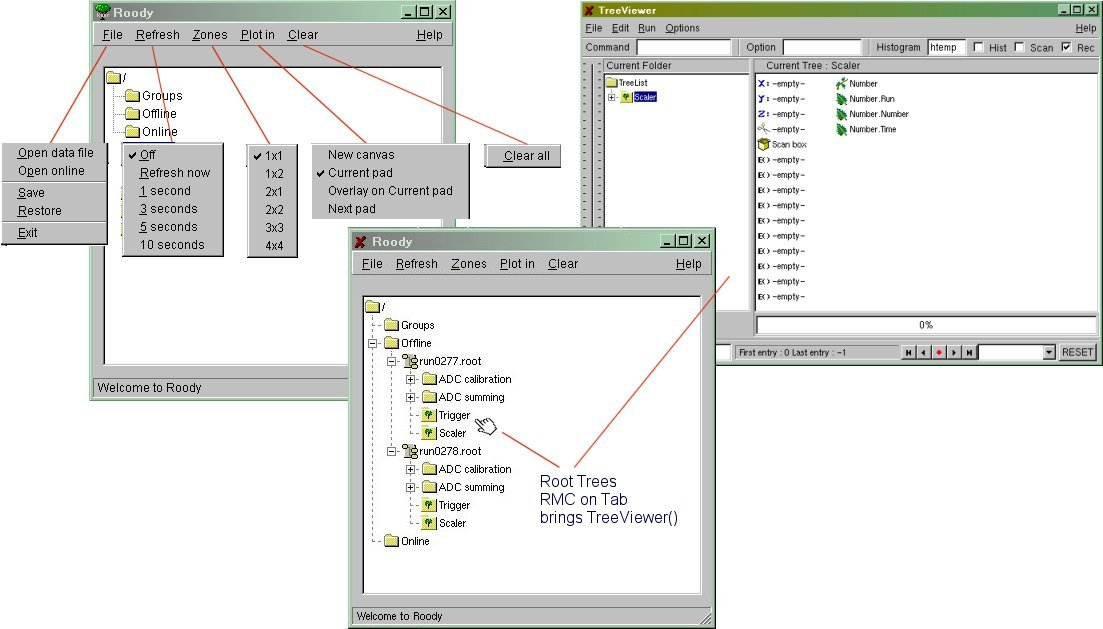
\includegraphics[width=8cm]{roody-sc-main}
\caption{Selection Convas Menu listing.}
\end{DoxyImage}
 \end{center} 

The menu list of the Selection Canvas is specific to \doxyref{Roody}{p.}{classRoody}.
\begin{DoxyItemize}
\item {\bfseries  File }
\begin{DoxyItemize}
\item {\bfseries  Open data file } : Open {\itshape file.root\/} or {\itshape file.hbook\/}. Opened files will be placed under the {\itshape offline\/} Tab in SC (see \doxyref{Open file}{p.}{features_open}).
\item {\bfseries  Open online } : Open network connection to a running analyzer. Requires host and socket port number for activating the connection. Link to online analyzer will be placed under the {\itshape online\/} Tab in the SC (see \doxyref{Online use}{p.}{features_online}).
\item {\bfseries  Save } : Save the overall configuration of the \doxyref{Roody}{p.}{classRoody} application into a XML file description (see \doxyref{Save option}{p.}{features_save}).
\item {\bfseries  Restore } : Restore from a previously saved XML configuration the \doxyref{Roody}{p.}{classRoody} settings (see \doxyref{Restore option}{p.}{features_restore})
\end{DoxyItemize}
\item {\bfseries  Refresh } : see \doxyref{Refresh option}{p.}{features_refresh}
\begin{DoxyItemize}
\item {\bfseries  Off } : Deactivate the automatic histogram content refresh for the {\itshape online\/} connection.
\item {\bfseries  Refresh now } : Force an update of the current histogram display content for the {\itshape online\/} connection.
\item {\bfseries  n seconds } : Activate the automatic histogram content refresh based on the time interval selection.
\end{DoxyItemize}
\item {\bfseries  Zone } : see \doxyref{Zones option}{p.}{features_zone}
\begin{DoxyItemize}
\item {\bfseries  j x k } : Define the canvas configuration for the upcoming histogram display request.
\end{DoxyItemize}
\item {\bfseries  Plot in } : see \doxyref{Plot option}{p.}{features_plot}
\begin{DoxyItemize}
\item {\bfseries  New Canvas } : When selecting a histogram for display, force its appearance in a new canvas.
\item {\bfseries  Current Pad } : Replace the current histogram with newly selected one. If no canvas is available, a new canvas with the default zone setting will be created.
\item {\bfseries  Overlay on Current Pad } : Overlay the selected histogram on the current displayed pad.
\item {\bfseries  Next Pad } : When selecting a histogram for display, force its appearance into the next pad of the canvas. In the case the canvas has only one pad, replace its content.
\end{DoxyItemize}
\item {\bfseries  Clear } : Clear the content of {\bfseries all} the histograms of the {\bfseries online} connection.
\end{DoxyItemize}



 \subsection{Open file}\label{features_open}

\begin{DoxyEnumerate}
\item There is 3 different ways to open {\itshape files:\/} 
\begin{DoxyEnumerate}
\item When invoking the roody application through the argument list
\begin{DoxyItemize}
\item Start roody with multiple root files. 
\begin{DoxyCode}
    > roody run0277.root run0278.root
\end{DoxyCode}
 \begin{center} Multiple root file from argument.  
\begin{DoxyImage}
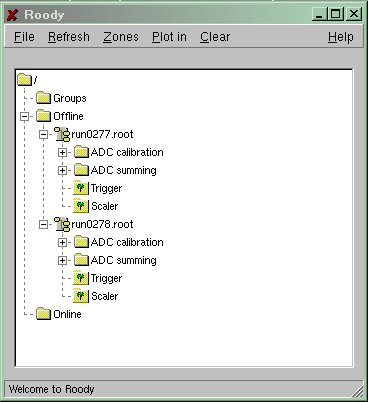
\includegraphics[width=8cm]{roody-inter}
\caption{Multiple root file from argument.}
\end{DoxyImage}
 \end{center}  ...
\end{DoxyItemize}
\item Right mouse click on the offline tab -\/$>$ Select file
\begin{DoxyItemize}
\item Right Click on the {\bfseries offline} tab. The File selector will appear. ... \begin{center}  
\begin{DoxyImageNoCaption}
  \mbox{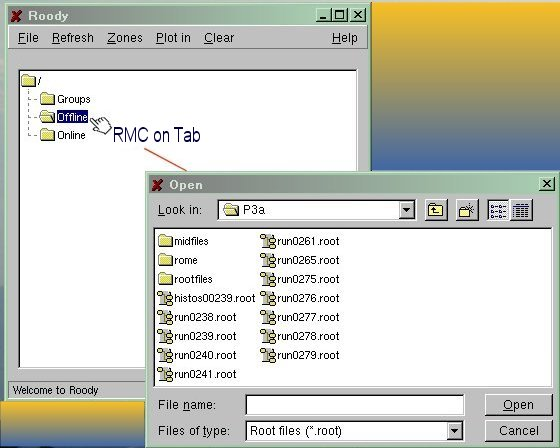
\includegraphics[width=6cm]{roody-open-01}}
\end{DoxyImageNoCaption}
 \end{center}  ...
\end{DoxyItemize}
\item From the pull-\/down menu of the roody application
\begin{DoxyItemize}
\item File -\/$>$ open data file -\/$>$ Select file
\end{DoxyItemize}
\end{DoxyEnumerate}
\end{DoxyEnumerate}



 \subsection{Close file}\label{features_close}

\begin{DoxyEnumerate}
\item There is one way to close an opened file within \doxyref{Roody}{p.}{classRoody}
\begin{DoxyItemize}
\item Right Click on the file name tab, a \char`\"{}close file\char`\"{} will appear to active the closure.
\end{DoxyItemize}
\end{DoxyEnumerate}

\begin{center}  
\begin{DoxyImageNoCaption}
  \mbox{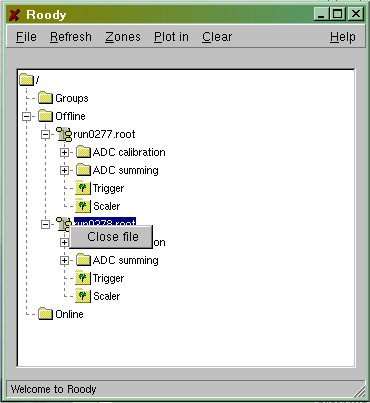
\includegraphics[width=6cm]{roody-close-01}}
\end{DoxyImageNoCaption}
 \end{center}  ... 

 \subsection{Save option}\label{features_save}
This option provides currently the mean of saving the online connection and the group assignments into a .XML file. In the future, this option will be extended to include also the GC content and their positions. The format of the .XML follows the DTD scheme. 
\begin{DoxyCode}
<?xml version="1.0" encoding="ISO-8859-1"?>
<!DOCTYPE roody SYSTEM "roody.dtd">

<!-- created by Roody on Thu Nov 04 22:10:14 2004 -->

<roody>
  <file>C:\Projects\p3a\histos00265.root</file>
  <group>
    <name>MyGroup</name>
    <histogram>
      <name>hTDC_001</name>
      <source>C:\Projects\p3a\histos00265.root</source>
    </histogram>
    <histogram>
      <name>hTDC_002</name>
      <source>C:\Projects\p3a\histos00265.root</source>
    </histogram>
    <histogram>
      <name>hTDC_003</name>
      <source>C:\Projects\p3a\histos00265.root</source>
    </histogram>
    <histogram>
      <name>hTDC_004</name>
      <source>C:\Projects\p3a\histos00265.root</source>
    </histogram>
  </group>
</roody>
\end{DoxyCode}




 \subsection{Restore option}\label{features_restore}
This option is to recover saved online connection and group definitions saved previously through the File-\/$>$Save pull-\/down menu. This .XML file can be requested at the execution of the \doxyref{Roody}{p.}{classRoody} application through argument.



 \subsection{Refresh option}\label{features_refresh}
Valid option only for \doxyref{Online use}{p.}{features_online} connection. Allows the automatic refresh of all active GC. Currently the refresh is not disabled while you're picking up the limits for a zoom. In the case the refresh is set to a short time interval this operation (X or Y scaling) is cancelled as the refresh is performed. Make sure to manually disable or extend the refresh option before doing this operation.



 \subsection{Zones option}\label{features_zone}
Predefined zone setting are available from the pull-\/down menu (2x2, 4x4, etc). Using the grouping method, the zone will be adjusted to fit the number of elements of your group. In the case the group contains a large number of elements, it could be advantageous to \char`\"{}zoom in\char`\"{} a single element. This is now possible by RMC on the pad of interest and selecting the {\bfseries ZoomOption}. A \char`\"{}ZoomOption\char`\"{} has been added to the context menu produced by right clicking anywhere on a histogram frame. This opens up a new canvas, titled \char`\"{}Zoom
Canvas\char`\"{}, containing a copy of the histogram in the original frame.



 \subsection{Plot option}\label{features_plot}
Global selection of the mode of display. This mode can be individualized with a RMC on the histogram Tab.

\begin{center} RMC on the hAll Tab  
\begin{DoxyImage}
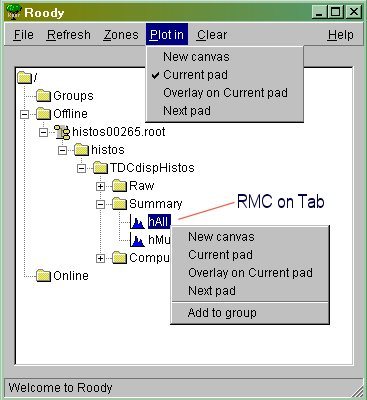
\includegraphics[width=6cm]{roody-plot}
\caption{RMC on the hAll Tab}
\end{DoxyImage}
 \end{center} 



 \section{Graphical Canvas}\label{features_gc}
This Graphical Canvas is the result of a DLMC on a Histogram Tab or Group Tab. The composition of this canvas will be dependent on the mode \doxyref{Zones option}{p.}{features_zone} selected...



 \subsection{Histogram display}\label{features_view}
The procedure to display histogram is independent of the source of the data. In either case {\bfseries Offline} or {\bfseries Online} the content of the source will be displayed in a hierarchical structure under the file name Tab. This content can be composed of folders, Tree or Histograms. You can expand the folders by DLMC the Folder Tab. By DLMC on any of the histogram name , a new window (GC) will appear on the back of the SC with the graphical representation of the histogram.

\begin{center} Main \doxyref{Roody}{p.}{classRoody} Selection Canvas (SC) with Graphical Canvas (GC).  
\begin{DoxyImage}
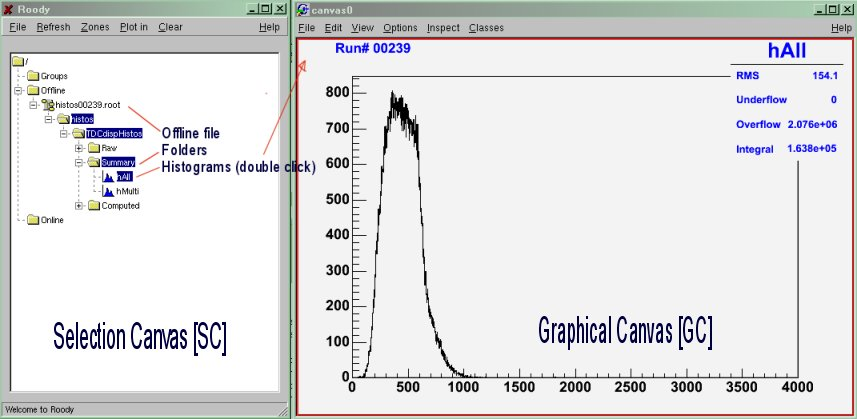
\includegraphics[width=6cm]{roody-hist-01}
\caption{Main Roody Selection Canvas (SC) with Graphical Canvas (GC)}
\end{DoxyImage}
 \end{center} 


\begin{DoxyEnumerate}
\item On the GC, standard ROOT options are applicable
\begin{DoxyItemize}
\item Tool bar can be activated from pull-\/down menu View-\/$>$Tool Bar. Provides ROOT icons on the top of the canvas
\item Event Status can be activated from pull-\/down menu View-\/$>$Event Status. Provides x/y coordinates and bin content of the bin under the mouse (mouse should be on the top of the bin).
\item Editor extention can be activated from pull-\/down menu View-\/$>$Editor. Provides on the left hand side Editor panel context sensitive to the Right Mouse Click location on the canvas.
\item Right Mouse click on the different colored zone on the figure below pop up specific set of options. Most used is the X/Y axis for X or Y \doxyref{X/Y Scaling}{p.}{features_scaling} Unzoom.
\end{DoxyItemize}
\end{DoxyEnumerate}

\begin{center}  
\begin{DoxyImageNoCaption}
  \mbox{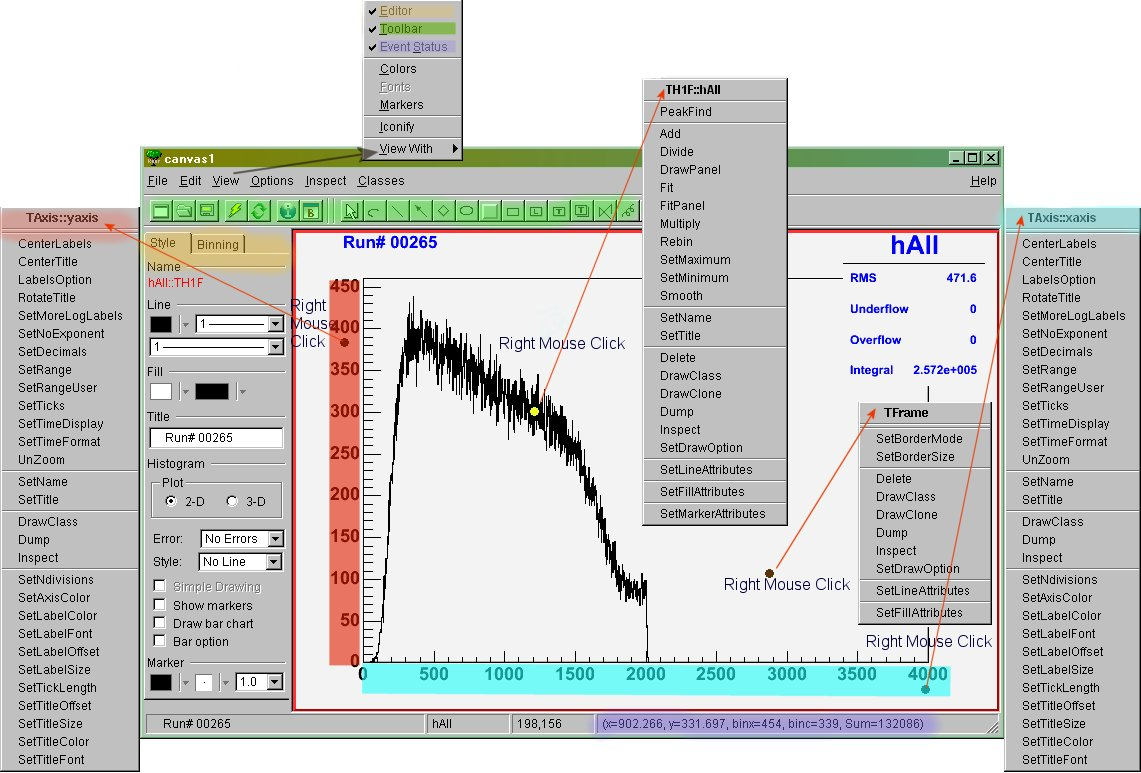
\includegraphics[width=6cm]{roody-gc-main}}
\end{DoxyImageNoCaption}
 \end{center} 



 \subsection{X/Y Scaling}\label{features_scaling}

\begin{DoxyItemize}
\item The X or Y scaling (zoom) can be achieved in several ways
\begin{DoxyEnumerate}
\item Using the mouse in the X or Y axis region (when hand mouse icon appears) by dragging the mouse along the region of interest.
\item Using the Editor extension panel for data selection under Bining.
\end{DoxyEnumerate}
\end{DoxyItemize}\subsubsection{X/Y-\/scale limits}\label{features_X-scale_limits}
To set the x/y-\/axis limits, right click anywhere on a histogram frame and choose \char`\"{}X/YaxisLimits\char`\"{} from the popup context menu. This brings up a dialog box where you can enter the x/ymin and x/ymax values. Click \char`\"{}OK\char`\"{} and all pads within the currently selected canvas will be redrawn with that x/y-\/axis scale. To reset all histograms so the x/y-\/axes are unzoomed, click \char`\"{}Unzoom\char`\"{}.\subsubsection{Y-\/scale freeze}\label{features_Y-scale_freeze}
The y-\/axis scales can now be fixed just like the x-\/axis scales. Choose {\bfseries YaxisLimits} from the context menu when RMC'ing on a histogram frame and a small dialog box will open in which you can enter the min and max values. If the frame is part of a multipad canvas, all pads on that canvas will be redrawn with the new scales. Choose {\bfseries YaxisLimits} again and click on the Unzoom button to unzoom all pads on that canvas.



 \subsection{Peak Finder}\label{features_peakfinder}

\begin{DoxyItemize}
\item The option is invoked from the RMC
\end{DoxyItemize}



 \section{Group use}\label{features_group}
The intent of the group is to give the possibility to gather multiple histograms under a single group name for fast display. Independently of the number of histograms, when the group is requested for display, the canvas will be split accordingly.

The procedure to use a group is the following:


\begin{DoxyEnumerate}
\item Create a group: RMC on the Group Tab, select {\bfseries  Make new group }, enter a group name.
\item Add histogram to a group:
\begin{DoxyItemize}
\item RMC on the histogram Tab to add to the group, select {\bfseries  Add to group } select the group to place the histogram into. If only one group is created, the group selection will be omitted.
\item For multiple histogram selection, hold the CTL key down while selecting the histograms. When the selection is complete, {\bfseries Hold} the CTL key {\bfseries and} RMC for the {\bfseries  Add to group }.
\end{DoxyItemize}
\item Check a group\_\-name content: DLMC the Group Tab to see the newly created group\_\-name. DLMC the group\_\-name to list its content.
\item Display a group: RMC on the group\_\-name and select {\bfseries  Draw group }. This will create a new canvas will zone up to the number of histograms of that group or update a previously displayed canvas of that group\_\-name.
\item Delete a group\_\-name: RMC on the group\_\-name, select {\bfseries  Delete group }.
\end{DoxyEnumerate}


\begin{DoxyItemize}
\item The list of group\_\-name can be saved (\doxyref{Save option}{p.}{features_save}) into a file for later restoration (see \doxyref{Restore option}{p.}{features_restore})..
\end{DoxyItemize}

\begin{center}  
\begin{DoxyImageNoCaption}
  \mbox{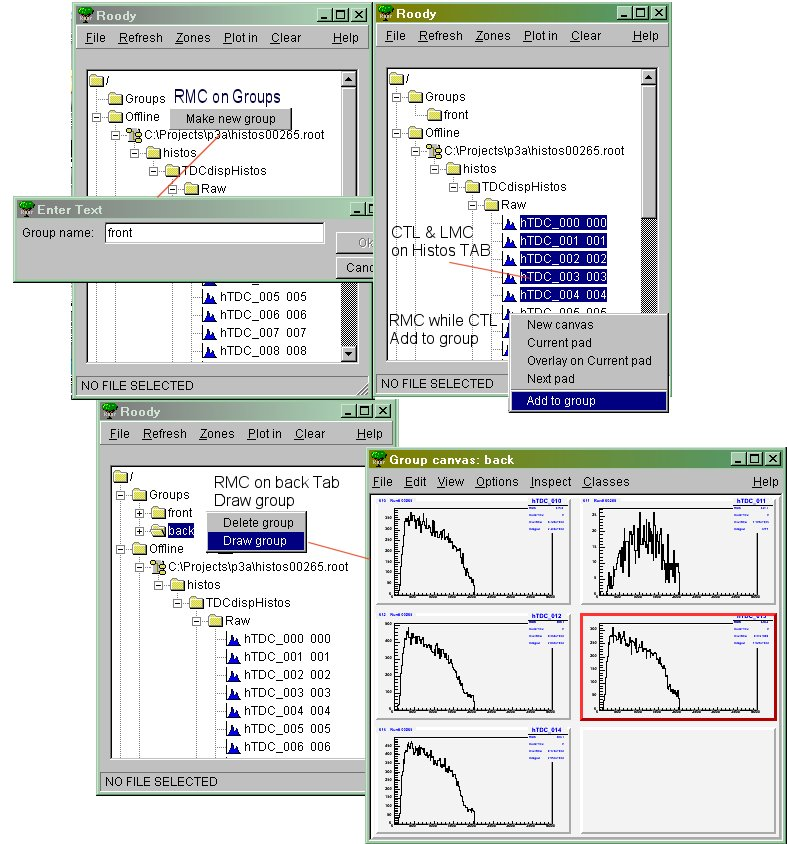
\includegraphics[width=6cm]{roody-group}}
\end{DoxyImageNoCaption}
 \end{center} 



 \section{Offline use}\label{features_offline}
The Offline Tab is to gather all the offline files opened through the \doxyref{Roody}{p.}{classRoody} application. ...



 \section{Online use}\label{features_online}
Under the Online Tab, the online connection request will be expended with the corresponding histograms retrieved through this network channel. ...

\par
  \doxyref{Quickstart}{p.}{quickstart} -\/ \doxyref{top}{p.}{index_top} -\/ \doxyref{top}{p.}{index_top}  
\chapter{Quickstart}
\label{quickstart}
 intro -\/ \doxyref{top}{p.}{index_top} -\/ \doxyref{Features}{p.}{features} 

Please refer to the {\tt README} file.

 intro -\/ \doxyref{top}{p.}{index_top} -\/ \doxyref{Features}{p.}{features}  
\chapter{Directory Hierarchy}
\section{Directories}
This directory hierarchy is sorted roughly, but not completely, alphabetically:\begin{DoxyCompactList}
\item \contentsline{section}{include}{\pageref{dir_36090cc217820b1f4a76b73f6461e1dc}}{}
\item \contentsline{section}{src}{\pageref{dir_ffd95fa52d9bc5b54d53164b5d5f7e0b}}{}
\end{DoxyCompactList}

\chapter{Class Index}
\section{Class List}
Here are the classes, structs, unions and interfaces with brief descriptions:\begin{DoxyCompactList}
\item\contentsline{section}{{\bf MemDebug} }{\pageref{classMemDebug}}{}
\item\contentsline{section}{{\bf MTGListTree} }{\pageref{classMTGListTree}}{}
\item\contentsline{section}{{\bf OptStatMenu} }{\pageref{classOptStatMenu}}{}
\item\contentsline{section}{{\bf PadObject} }{\pageref{structPadObject}}{}
\item\contentsline{section}{{\bf PadObjectVec} }{\pageref{structPadObjectVec}}{}
\item\contentsline{section}{{\bf Roody} }{\pageref{classRoody}}{}
\item\contentsline{section}{{\bf RoodyXML} }{\pageref{classRoodyXML}}{}
\item\contentsline{section}{{\bf TGTextDialog} }{\pageref{classTGTextDialog}}{}
\item\contentsline{section}{{\bf TPeakFindPanel} }{\pageref{classTPeakFindPanel}}{}
\end{DoxyCompactList}

\chapter{File Index}
\subsection{File List}
Here is a list of all files with brief descriptions:\begin{DoxyCompactList}
\item\contentsline{section}{\hyperlink{adccalib_8c}{adccalib.c} }{\pageref{adccalib_8c}}{}
\item\contentsline{section}{\hyperlink{adcsum_8c}{adcsum.c} }{\pageref{adcsum_8c}}{}
\item\contentsline{section}{\hyperlink{alarm_8c}{alarm.c} }{\pageref{alarm_8c}}{}
\item\contentsline{section}{\hyperlink{analyzer_8c}{analyzer.c} }{\pageref{analyzer_8c}}{}
\item\contentsline{section}{\hyperlink{cnaf__callback_8c}{cnaf\_\-callback.c} }{\pageref{cnaf__callback_8c}}{}
\item\contentsline{section}{\hyperlink{ebuser_8c}{ebuser.c} }{\pageref{ebuser_8c}}{}
\item\contentsline{section}{\hyperlink{elog_8c}{elog.c} }{\pageref{elog_8c}}{}
\item\contentsline{section}{\hyperlink{esone_8c}{esone.c} }{\pageref{esone_8c}}{}
\item\contentsline{section}{\hyperlink{experim_8h}{experim.h} }{\pageref{experim_8h}}{}
\item\contentsline{section}{\hyperlink{fevme_8cxx}{fevme.cxx} }{\pageref{fevme_8cxx}}{}
\item\contentsline{section}{\hyperlink{fevmemodules_8c}{fevmemodules.c} }{\pageref{fevmemodules_8c}}{}
\item\contentsline{section}{\hyperlink{frontend_8c}{frontend.c} }{\pageref{frontend_8c}}{}
\item\contentsline{section}{\hyperlink{history_8c}{history.c} }{\pageref{history_8c}}{}
\item\contentsline{section}{\hyperlink{hv_8c}{hv.c} }{\pageref{hv_8c}}{}
\item\contentsline{section}{\hyperlink{isegvhs_8c}{isegvhs.c} }{\pageref{isegvhs_8c}}{}
\item\contentsline{section}{\hyperlink{isegvhs_8h}{isegvhs.h} }{\pageref{isegvhs_8h}}{}
\item\contentsline{section}{\hyperlink{isegvhsdrv_8h}{isegvhsdrv.h} }{\pageref{isegvhsdrv_8h}}{}
\item\contentsline{section}{\hyperlink{lrs1151_8c}{lrs1151.c} }{\pageref{lrs1151_8c}}{}
\item\contentsline{section}{\hyperlink{lrs1151_8h}{lrs1151.h} }{\pageref{lrs1151_8h}}{}
\item\contentsline{section}{\hyperlink{lrs1190_8c}{lrs1190.c} }{\pageref{lrs1190_8c}}{}
\item\contentsline{section}{\hyperlink{lrs1190_8h}{lrs1190.h} }{\pageref{lrs1190_8h}}{}
\item\contentsline{section}{\hyperlink{Makefile}{Makefile} }{\pageref{Makefile}}{}
\item\contentsline{section}{\hyperlink{mcstd_8h}{mcstd.h} }{\pageref{mcstd_8h}}{}
\item\contentsline{section}{\hyperlink{mdsupport_8c}{mdsupport.c} }{\pageref{mdsupport_8c}}{}
\item\contentsline{section}{\hyperlink{mdsupport_8h}{mdsupport.h} }{\pageref{mdsupport_8h}}{}
\item\contentsline{section}{\hyperlink{mesadc32_8c}{mesadc32.c} }{\pageref{mesadc32_8c}}{}
\item\contentsline{section}{\hyperlink{mesadc32_8h}{mesadc32.h} }{\pageref{mesadc32_8h}}{}
\item\contentsline{section}{\hyperlink{mesadc32drv_8h}{mesadc32drv.h} }{\pageref{mesadc32drv_8h}}{}
\item\contentsline{section}{\hyperlink{mevb_8c}{mevb.c} }{\pageref{mevb_8c}}{}
\item\contentsline{section}{\hyperlink{mfe_8c}{mfe.c} }{\pageref{mfe_8c}}{}
\item\contentsline{section}{\hyperlink{midas_8c}{midas.c} }{\pageref{midas_8c}}{}
\item\contentsline{section}{\hyperlink{midas_8h}{midas.h} }{\pageref{midas_8h}}{}
\item\contentsline{section}{\hyperlink{mrpc_8c}{mrpc.c} }{\pageref{mrpc_8c}}{}
\item\contentsline{section}{\hyperlink{mrpc_8h}{mrpc.h} }{\pageref{mrpc_8h}}{}
\item\contentsline{section}{\hyperlink{msystem_8h}{msystem.h} }{\pageref{msystem_8h}}{}
\item\contentsline{section}{\hyperlink{mvmestd_8h}{mvmestd.h} }{\pageref{mvmestd_8h}}{}
\item\contentsline{section}{\hyperlink{myexpt_8html}{myexpt.html} }{\pageref{myexpt_8html}}{}
\item\contentsline{section}{\hyperlink{odb_8c}{odb.c} }{\pageref{odb_8c}}{}
\item\contentsline{section}{\hyperlink{ov1720_8c}{ov1720.c} }{\pageref{ov1720_8c}}{}
\item\contentsline{section}{\hyperlink{ov1720drv_8h}{ov1720drv.h} }{\pageref{ov1720drv_8h}}{}
\item\contentsline{section}{\hyperlink{ov1740_8c}{ov1740.c} }{\pageref{ov1740_8c}}{}
\item\contentsline{section}{\hyperlink{ov1740drv_8h}{ov1740drv.h} }{\pageref{ov1740drv_8h}}{}
\item\contentsline{section}{\hyperlink{scaler_8c}{scaler.c} }{\pageref{scaler_8c}}{}
\item\contentsline{section}{\hyperlink{sis3320_8c}{sis3320.c} }{\pageref{sis3320_8c}}{}
\item\contentsline{section}{\hyperlink{sis3320_8h}{sis3320.h} }{\pageref{sis3320_8h}}{}
\item\contentsline{section}{\hyperlink{sis3320drv_8h}{sis3320drv.h} }{\pageref{sis3320drv_8h}}{}
\item\contentsline{section}{\hyperlink{sis3801_8c}{sis3801.c} }{\pageref{sis3801_8c}}{}
\item\contentsline{section}{\hyperlink{sis3801_8h}{sis3801.h} }{\pageref{sis3801_8h}}{}
\item\contentsline{section}{\hyperlink{sis3803_8c}{sis3803.c} }{\pageref{sis3803_8c}}{}
\item\contentsline{section}{\hyperlink{sis3803_8h}{sis3803.h} }{\pageref{sis3803_8h}}{}
\item\contentsline{section}{\hyperlink{sis3820_8c}{sis3820.c} }{\pageref{sis3820_8c}}{}
\item\contentsline{section}{\hyperlink{sis3820_8h}{sis3820.h} }{\pageref{sis3820_8h}}{}
\item\contentsline{section}{\hyperlink{sis3820drv_8h}{sis3820drv.h} }{\pageref{sis3820drv_8h}}{}
\item\contentsline{section}{\hyperlink{system_8c}{system.c} }{\pageref{system_8c}}{}
\item\contentsline{section}{\hyperlink{v1190B_8c}{v1190B.c} }{\pageref{v1190B_8c}}{}
\item\contentsline{section}{\hyperlink{v1190B_8h}{v1190B.h} }{\pageref{v1190B_8h}}{}
\item\contentsline{section}{\hyperlink{v1720_8c}{v1720.c} }{\pageref{v1720_8c}}{}
\item\contentsline{section}{\hyperlink{v1720_8h}{v1720.h} }{\pageref{v1720_8h}}{}
\item\contentsline{section}{\hyperlink{v1720drv_8h}{v1720drv.h} }{\pageref{v1720drv_8h}}{}
\item\contentsline{section}{\hyperlink{v1729_8c}{v1729.c} }{\pageref{v1729_8c}}{}
\item\contentsline{section}{\hyperlink{v1729_8h}{v1729.h} }{\pageref{v1729_8h}}{}
\item\contentsline{section}{\hyperlink{v1740_8c}{v1740.c} }{\pageref{v1740_8c}}{}
\item\contentsline{section}{\hyperlink{v1740_8h}{v1740.h} }{\pageref{v1740_8h}}{}
\item\contentsline{section}{\hyperlink{v1740drv_8h}{v1740drv.h} }{\pageref{v1740drv_8h}}{}
\item\contentsline{section}{\hyperlink{v513_8c}{v513.c} }{\pageref{v513_8c}}{}
\item\contentsline{section}{\hyperlink{v513_8h}{v513.h} }{\pageref{v513_8h}}{}
\item\contentsline{section}{\hyperlink{v560_8c}{v560.c} }{\pageref{v560_8c}}{}
\item\contentsline{section}{\hyperlink{v560_8h}{v560.h} }{\pageref{v560_8h}}{}
\item\contentsline{section}{\hyperlink{v792_8c}{v792.c} }{\pageref{v792_8c}}{}
\item\contentsline{section}{\hyperlink{v792_8h}{v792.h} }{\pageref{v792_8h}}{}
\item\contentsline{section}{\hyperlink{v895_8h}{v895.h} }{\pageref{v895_8h}}{}
\item\contentsline{section}{\hyperlink{vmeio_8c}{vmeio.c} }{\pageref{vmeio_8c}}{}
\item\contentsline{section}{\hyperlink{vmeio_8h}{vmeio.h} }{\pageref{vmeio_8h}}{}
\item\contentsline{section}{\hyperlink{vpc6_8c}{vpc6.c} }{\pageref{vpc6_8c}}{}
\item\contentsline{section}{\hyperlink{vpc6_8h}{vpc6.h} }{\pageref{vpc6_8h}}{}
\item\contentsline{section}{\hyperlink{vppg_8c}{vppg.c} }{\pageref{vppg_8c}}{}
\item\contentsline{section}{\hyperlink{vppg_8h}{vppg.h} }{\pageref{vppg_8h}}{}
\item\contentsline{section}{\hyperlink{vt2_8c}{vt2.c} }{\pageref{vt2_8c}}{}
\item\contentsline{section}{\hyperlink{vt2_8h}{vt2.h} }{\pageref{vt2_8h}}{}
\item\contentsline{section}{\hyperlink{vt48_8c}{vt48.c} }{\pageref{vt48_8c}}{}
\item\contentsline{section}{\hyperlink{vt48_8h}{vt48.h} }{\pageref{vt48_8h}}{}
\item\contentsline{section}{\hyperlink{xcustom_8odb}{xcustom.odb} }{\pageref{xcustom_8odb}}{}
\end{DoxyCompactList}

\chapter{Directory Documentation}
\section{/home/nam/sw/daq/roody/include/ Directory Reference}
\label{dir_36090cc217820b1f4a76b73f6461e1dc}\index{/home/nam/sw/daq/roody/include/ Directory Reference@{/home/nam/sw/daq/roody/include/ Directory Reference}}
\subsection*{Files}
\begin{DoxyCompactItemize}
\item 
file {\bf MTGListTree.h}
\item 
file {\bf Roody.h}
\item 
file {\bf RoodyXML.h}
\item 
file {\bf TGTextDialog.h}
\item 
file {\bf TPeakFindPanel.h}
\end{DoxyCompactItemize}

\section{/home/nam/sw/daq/roody/src/ Directory Reference}
\label{dir_ffd95fa52d9bc5b54d53164b5d5f7e0b}\index{/home/nam/sw/daq/roody/src/ Directory Reference@{/home/nam/sw/daq/roody/src/ Directory Reference}}
\subsection*{Files}
\begin{DoxyCompactItemize}
\item 
file {\bf MTGListTree.cxx}
\item 
file {\bf Roody.cxx}
\item 
file {\bf RoodyXML.cxx}
\item 
file {\bf TGTextDialog.cxx}
\end{DoxyCompactItemize}

\chapter{Class Documentation}
\section{MemDebug Class Reference}
\label{classMemDebug}\index{MemDebug@{MemDebug}}
\subsection*{Public Member Functions}
\begin{DoxyCompactItemize}
\item 
{\bf MemDebug} ()
\item 
{\bf $\sim$MemDebug} ()
\item 
TObject $\ast$ {\bf Clone} ()
\end{DoxyCompactItemize}


\subsection{Detailed Description}


Definition at line 58 of file Roody.cxx.



\subsection{Constructor \& Destructor Documentation}
\index{MemDebug@{MemDebug}!MemDebug@{MemDebug}}
\index{MemDebug@{MemDebug}!MemDebug@{MemDebug}}
\subsubsection[{MemDebug}]{\setlength{\rightskip}{0pt plus 5cm}MemDebug::MemDebug (
\begin{DoxyParamCaption}
{}
\end{DoxyParamCaption}
)\hspace{0.3cm}{\ttfamily  [inline]}}\label{classMemDebug_a3ae05e40241f29fafc75ecb666285cf7}


Definition at line 62 of file Roody.cxx.



Referenced by Clone().

\index{MemDebug@{MemDebug}!$\sim$MemDebug@{$\sim$MemDebug}}
\index{$\sim$MemDebug@{$\sim$MemDebug}!MemDebug@{MemDebug}}
\subsubsection[{$\sim$MemDebug}]{\setlength{\rightskip}{0pt plus 5cm}MemDebug::$\sim$MemDebug (
\begin{DoxyParamCaption}
{}
\end{DoxyParamCaption}
)\hspace{0.3cm}{\ttfamily  [inline]}}\label{classMemDebug_a1d31b9a076202000b27e2b4f7641fef5}


Definition at line 67 of file Roody.cxx.



\subsection{Member Function Documentation}
\index{MemDebug@{MemDebug}!Clone@{Clone}}
\index{Clone@{Clone}!MemDebug@{MemDebug}}
\subsubsection[{Clone}]{\setlength{\rightskip}{0pt plus 5cm}TObject$\ast$ MemDebug::Clone (
\begin{DoxyParamCaption}
{}
\end{DoxyParamCaption}
)\hspace{0.3cm}{\ttfamily  [inline]}}\label{classMemDebug_a393888af02ddd6f540992ea8f1bc9c00}


Definition at line 73 of file Roody.cxx.



The documentation for this class was generated from the following file:\begin{DoxyCompactItemize}
\item 
{\bf Roody.cxx}\end{DoxyCompactItemize}

\section{MTGListTree Class Reference}
\label{classMTGListTree}\index{MTGListTree@{MTGListTree}}


{\ttfamily \#include $<$MTGListTree.h$>$}

\subsection*{Public Member Functions}
\begin{DoxyCompactItemize}
\item 
{\bf MTGListTree} (TGWindow $\ast$, UInt\_\-t, UInt\_\-t, UInt\_\-t, ULong\_\-t=GetWhitePixel())
\item 
{\bf MTGListTree} (TGCanvas $\ast$, UInt\_\-t, ULong\_\-t=GetWhitePixel())
\item 
Bool\_\-t {\bf HandleButton} (Event\_\-t $\ast$)
\item 
Bool\_\-t {\bf HandleKey} (Event\_\-t $\ast$)
\item 
void {\bf GetSelectedItems} (std::vector$<$ TGListTreeItem $\ast$ $>$ \&)
\item 
void {\bf GetSelectedItemsRecursive} (TGListTreeItem $\ast$, std::vector$<$ TGListTreeItem $\ast$ $>$ \&)
\item 
Int\_\-t {\bf MDeleteItem} (TGListTreeItem $\ast$)
\item 
void {\bf MPDeleteChildren} (TGListTreeItem $\ast$)
\end{DoxyCompactItemize}
\subsection*{Private Types}
\begin{DoxyCompactItemize}
\item 
typedef std::vector$<$ TGListTreeItem $\ast$ $>$::{\bf iterator} {\bf iterator}
\end{DoxyCompactItemize}
\subsection*{Private Member Functions}
\begin{DoxyCompactItemize}
\item 
void {\bf init} ()
\end{DoxyCompactItemize}
\subsection*{Private Attributes}
\begin{DoxyCompactItemize}
\item 
Bool\_\-t {\bf fControlPressed}
\end{DoxyCompactItemize}
\subsection*{Friends}
\begin{DoxyCompactItemize}
\item 
class {\bf TGListTreeItem}
\end{DoxyCompactItemize}


\subsection{Detailed Description}


Definition at line 17 of file MTGListTree.h.



\subsection{Member Typedef Documentation}
\index{MTGListTree@{MTGListTree}!iterator@{iterator}}
\index{iterator@{iterator}!MTGListTree@{MTGListTree}}
\subsubsection[{iterator}]{\setlength{\rightskip}{0pt plus 5cm}typedef std::vector$<$TGListTreeItem$\ast$$>$::{\bf iterator} {\bf MTGListTree::iterator}\hspace{0.3cm}{\ttfamily  [private]}}\label{classMTGListTree_a5d149669aa7aa7a9250cd204768d9129}


Definition at line 22 of file MTGListTree.h.



\subsection{Constructor \& Destructor Documentation}
\index{MTGListTree@{MTGListTree}!MTGListTree@{MTGListTree}}
\index{MTGListTree@{MTGListTree}!MTGListTree@{MTGListTree}}
\subsubsection[{MTGListTree}]{\setlength{\rightskip}{0pt plus 5cm}MTGListTree::MTGListTree (
\begin{DoxyParamCaption}
\item[{TGWindow $\ast$}]{p, }
\item[{UInt\_\-t}]{w, }
\item[{UInt\_\-t}]{h, }
\item[{UInt\_\-t}]{options, }
\item[{ULong\_\-t}]{back = {\ttfamily GetWhitePixel()}}
\end{DoxyParamCaption}
)}\label{classMTGListTree_ad8ac02718266588f1851521765feb9b7}


Definition at line 42 of file MTGListTree.cxx.

\index{MTGListTree@{MTGListTree}!MTGListTree@{MTGListTree}}
\index{MTGListTree@{MTGListTree}!MTGListTree@{MTGListTree}}
\subsubsection[{MTGListTree}]{\setlength{\rightskip}{0pt plus 5cm}MTGListTree::MTGListTree (
\begin{DoxyParamCaption}
\item[{TGCanvas $\ast$}]{p, }
\item[{UInt\_\-t}]{options, }
\item[{ULong\_\-t}]{back = {\ttfamily GetWhitePixel()}}
\end{DoxyParamCaption}
)}\label{classMTGListTree_ad0a89f242825cc021a560796533702b4}


Definition at line 47 of file MTGListTree.cxx.



\subsection{Member Function Documentation}
\index{MTGListTree@{MTGListTree}!GetSelectedItems@{GetSelectedItems}}
\index{GetSelectedItems@{GetSelectedItems}!MTGListTree@{MTGListTree}}
\subsubsection[{GetSelectedItems}]{\setlength{\rightskip}{0pt plus 5cm}void MTGListTree::GetSelectedItems (
\begin{DoxyParamCaption}
\item[{std::vector$<$ TGListTreeItem $\ast$ $>$ \&}]{items}
\end{DoxyParamCaption}
)}\label{classMTGListTree_a959170a63b6fb0a2c17944f6316743ce}


Definition at line 146 of file MTGListTree.cxx.



Referenced by Roody::ProcessMessage().

\index{MTGListTree@{MTGListTree}!GetSelectedItemsRecursive@{GetSelectedItemsRecursive}}
\index{GetSelectedItemsRecursive@{GetSelectedItemsRecursive}!MTGListTree@{MTGListTree}}
\subsubsection[{GetSelectedItemsRecursive}]{\setlength{\rightskip}{0pt plus 5cm}void MTGListTree::GetSelectedItemsRecursive (
\begin{DoxyParamCaption}
\item[{TGListTreeItem $\ast$}]{item, }
\item[{std::vector$<$ TGListTreeItem $\ast$ $>$ \&}]{items}
\end{DoxyParamCaption}
)}\label{classMTGListTree_ae4574857d80369d1acf9df42ab38d331}


Definition at line 153 of file MTGListTree.cxx.



Referenced by GetSelectedItems().

\index{MTGListTree@{MTGListTree}!HandleButton@{HandleButton}}
\index{HandleButton@{HandleButton}!MTGListTree@{MTGListTree}}
\subsubsection[{HandleButton}]{\setlength{\rightskip}{0pt plus 5cm}Bool\_\-t MTGListTree::HandleButton (
\begin{DoxyParamCaption}
\item[{Event\_\-t $\ast$}]{event}
\end{DoxyParamCaption}
)}\label{classMTGListTree_aa653659e11fde3d1675254c0a49416bc}


Definition at line 91 of file MTGListTree.cxx.

\index{MTGListTree@{MTGListTree}!HandleKey@{HandleKey}}
\index{HandleKey@{HandleKey}!MTGListTree@{MTGListTree}}
\subsubsection[{HandleKey}]{\setlength{\rightskip}{0pt plus 5cm}Bool\_\-t MTGListTree::HandleKey (
\begin{DoxyParamCaption}
\item[{Event\_\-t $\ast$}]{event}
\end{DoxyParamCaption}
)}\label{classMTGListTree_add074bbcb2d9d8cd4227112c0178a592}


Definition at line 164 of file MTGListTree.cxx.

\index{MTGListTree@{MTGListTree}!init@{init}}
\index{init@{init}!MTGListTree@{MTGListTree}}
\subsubsection[{init}]{\setlength{\rightskip}{0pt plus 5cm}void MTGListTree::init (
\begin{DoxyParamCaption}
{}
\end{DoxyParamCaption}
)\hspace{0.3cm}{\ttfamily  [private]}}\label{classMTGListTree_a9da47702de6d2875f4180ff793805701}


Referenced by MTGListTree().

\index{MTGListTree@{MTGListTree}!MDeleteItem@{MDeleteItem}}
\index{MDeleteItem@{MDeleteItem}!MTGListTree@{MTGListTree}}
\subsubsection[{MDeleteItem}]{\setlength{\rightskip}{0pt plus 5cm}Int\_\-t MTGListTree::MDeleteItem (
\begin{DoxyParamCaption}
\item[{TGListTreeItem $\ast$}]{item}
\end{DoxyParamCaption}
)}\label{classMTGListTree_a16442d4287e49070a09f9ba37b43d12c}


Definition at line 58 of file MTGListTree.cxx.



Referenced by Roody::CloseSource(), and Roody::DeleteGroup().

\index{MTGListTree@{MTGListTree}!MPDeleteChildren@{MPDeleteChildren}}
\index{MPDeleteChildren@{MPDeleteChildren}!MTGListTree@{MTGListTree}}
\subsubsection[{MPDeleteChildren}]{\setlength{\rightskip}{0pt plus 5cm}void MTGListTree::MPDeleteChildren (
\begin{DoxyParamCaption}
\item[{TGListTreeItem $\ast$}]{item}
\end{DoxyParamCaption}
)}\label{classMTGListTree_ab799a499555bfa3b17da435eb46e17e6}


Definition at line 71 of file MTGListTree.cxx.



Referenced by MDeleteItem().



\subsection{Friends And Related Function Documentation}
\index{MTGListTree@{MTGListTree}!TGListTreeItem@{TGListTreeItem}}
\index{TGListTreeItem@{TGListTreeItem}!MTGListTree@{MTGListTree}}
\subsubsection[{TGListTreeItem}]{\setlength{\rightskip}{0pt plus 5cm}friend class TGListTreeItem\hspace{0.3cm}{\ttfamily  [friend]}}\label{classMTGListTree_a5bda0cb7f07902080ed935fa1cd8d941}


Definition at line 19 of file MTGListTree.h.



Referenced by GetSelectedItems(), GetSelectedItemsRecursive(), HandleButton(), MDeleteItem(), and MPDeleteChildren().



\subsection{Member Data Documentation}
\index{MTGListTree@{MTGListTree}!fControlPressed@{fControlPressed}}
\index{fControlPressed@{fControlPressed}!MTGListTree@{MTGListTree}}
\subsubsection[{fControlPressed}]{\setlength{\rightskip}{0pt plus 5cm}Bool\_\-t {\bf MTGListTree::fControlPressed}\hspace{0.3cm}{\ttfamily  [private]}}\label{classMTGListTree_a5387e77c9a8fe1512d400294a8e8714f}


Definition at line 23 of file MTGListTree.h.



Referenced by HandleButton(), and HandleKey().



The documentation for this class was generated from the following files:\begin{DoxyCompactItemize}
\item 
{\bf MTGListTree.h}\item 
{\bf MTGListTree.cxx}\end{DoxyCompactItemize}

\section{OptStatMenu Class Reference}
\label{classOptStatMenu}\index{OptStatMenu@{OptStatMenu}}
\subsection*{Public Member Functions}
\begin{DoxyCompactItemize}
\item 
{\bf OptStatMenu} (const TGWindow $\ast$w)
\item 
Bool\_\-t {\bf ProcessMessage} (Long\_\-t msg, Long\_\-t parm1, Long\_\-t parm2)
\item 
void {\bf GetOptStat} ()
\item 
void {\bf SetOptStat} ()
\end{DoxyCompactItemize}


\subsection{Detailed Description}


Definition at line 794 of file Roody.cxx.



\subsection{Constructor \& Destructor Documentation}
\index{OptStatMenu@{OptStatMenu}!OptStatMenu@{OptStatMenu}}
\index{OptStatMenu@{OptStatMenu}!OptStatMenu@{OptStatMenu}}
\subsubsection[{OptStatMenu}]{\setlength{\rightskip}{0pt plus 5cm}OptStatMenu::OptStatMenu (
\begin{DoxyParamCaption}
\item[{const TGWindow $\ast$}]{w}
\end{DoxyParamCaption}
)\hspace{0.3cm}{\ttfamily  [inline]}}\label{classOptStatMenu_ada753399463dafcb4524be09fb54081f}


Definition at line 797 of file Roody.cxx.



\subsection{Member Function Documentation}
\index{OptStatMenu@{OptStatMenu}!GetOptStat@{GetOptStat}}
\index{GetOptStat@{GetOptStat}!OptStatMenu@{OptStatMenu}}
\subsubsection[{GetOptStat}]{\setlength{\rightskip}{0pt plus 5cm}void OptStatMenu::GetOptStat (
\begin{DoxyParamCaption}
{}
\end{DoxyParamCaption}
)\hspace{0.3cm}{\ttfamily  [inline]}}\label{classOptStatMenu_afed75c8a0cf3fd15ee05089ec5d8e6ab}


Definition at line 841 of file Roody.cxx.



Referenced by OptStatMenu().

\index{OptStatMenu@{OptStatMenu}!ProcessMessage@{ProcessMessage}}
\index{ProcessMessage@{ProcessMessage}!OptStatMenu@{OptStatMenu}}
\subsubsection[{ProcessMessage}]{\setlength{\rightskip}{0pt plus 5cm}Bool\_\-t OptStatMenu::ProcessMessage (
\begin{DoxyParamCaption}
\item[{Long\_\-t}]{msg, }
\item[{Long\_\-t}]{parm1, }
\item[{Long\_\-t}]{parm2}
\end{DoxyParamCaption}
)\hspace{0.3cm}{\ttfamily  [inline]}}\label{classOptStatMenu_a1410a4fc1c23c448651a2460b6e9a8c0}


Definition at line 821 of file Roody.cxx.

\index{OptStatMenu@{OptStatMenu}!SetOptStat@{SetOptStat}}
\index{SetOptStat@{SetOptStat}!OptStatMenu@{OptStatMenu}}
\subsubsection[{SetOptStat}]{\setlength{\rightskip}{0pt plus 5cm}void OptStatMenu::SetOptStat (
\begin{DoxyParamCaption}
{}
\end{DoxyParamCaption}
)\hspace{0.3cm}{\ttfamily  [inline]}}\label{classOptStatMenu_a7b24a69f8a79db451837e9a9e980be9d}


Definition at line 857 of file Roody.cxx.



Referenced by OptStatMenu(), and ProcessMessage().



The documentation for this class was generated from the following file:\begin{DoxyCompactItemize}
\item 
{\bf Roody.cxx}\end{DoxyCompactItemize}

\section{PadObject Struct Reference}
\label{structPadObject}\index{PadObject@{PadObject}}


{\ttfamily \#include $<$Roody.h$>$}

\subsection*{Public Member Functions}
\begin{DoxyCompactItemize}
\item 
{\bf PadObject} ()
\item 
{\bf PadObject} (int padnum, TObject $\ast$obj, const ObjectPath $\ast$src, const char $\ast$drawOption)
\item 
{\bf $\sim$PadObject} ()
\end{DoxyCompactItemize}
\subsection*{Public Attributes}
\begin{DoxyCompactItemize}
\item 
int {\bf fPadNumber}
\item 
TObject $\ast$ {\bf fObject}
\item 
ObjectPath {\bf fSource}
\item 
std::string {\bf fDrawOption}
\end{DoxyCompactItemize}


\subsection{Detailed Description}


Definition at line 35 of file Roody.h.



\subsection{Constructor \& Destructor Documentation}
\index{PadObject@{PadObject}!PadObject@{PadObject}}
\index{PadObject@{PadObject}!PadObject@{PadObject}}
\subsubsection[{PadObject}]{\setlength{\rightskip}{0pt plus 5cm}PadObject::PadObject (
\begin{DoxyParamCaption}
{}
\end{DoxyParamCaption}
)\hspace{0.3cm}{\ttfamily  [inline]}}\label{structPadObject_a0af56a6cdb687fda40758711e7117d37}


Definition at line 42 of file Roody.h.

\index{PadObject@{PadObject}!PadObject@{PadObject}}
\index{PadObject@{PadObject}!PadObject@{PadObject}}
\subsubsection[{PadObject}]{\setlength{\rightskip}{0pt plus 5cm}PadObject::PadObject (
\begin{DoxyParamCaption}
\item[{int}]{padnum, }
\item[{TObject $\ast$}]{obj, }
\item[{const ObjectPath $\ast$}]{src, }
\item[{const char $\ast$}]{drawOption}
\end{DoxyParamCaption}
)\hspace{0.3cm}{\ttfamily  [inline]}}\label{structPadObject_a285c91c90c38d5ad73fe4861a565b2f5}


Definition at line 43 of file Roody.h.

\index{PadObject@{PadObject}!$\sim$PadObject@{$\sim$PadObject}}
\index{$\sim$PadObject@{$\sim$PadObject}!PadObject@{PadObject}}
\subsubsection[{$\sim$PadObject}]{\setlength{\rightskip}{0pt plus 5cm}PadObject::$\sim$PadObject (
\begin{DoxyParamCaption}
{}
\end{DoxyParamCaption}
)\hspace{0.3cm}{\ttfamily  [inline]}}\label{structPadObject_a47f5972c71458c252b2feadd9c8511a0}


Definition at line 50 of file Roody.h.



\subsection{Member Data Documentation}
\index{PadObject@{PadObject}!fDrawOption@{fDrawOption}}
\index{fDrawOption@{fDrawOption}!PadObject@{PadObject}}
\subsubsection[{fDrawOption}]{\setlength{\rightskip}{0pt plus 5cm}std::string {\bf PadObject::fDrawOption}}\label{structPadObject_ab4a27ba00cd3669e80ab4b242c949db2}


Definition at line 40 of file Roody.h.



Referenced by Roody::AddPadToVec(), and PadObject().

\index{PadObject@{PadObject}!fObject@{fObject}}
\index{fObject@{fObject}!PadObject@{PadObject}}
\subsubsection[{fObject}]{\setlength{\rightskip}{0pt plus 5cm}TObject$\ast$ {\bf PadObject::fObject}}\label{structPadObject_a8032e91fa662ac8f50a13350083d401d}


Definition at line 38 of file Roody.h.



Referenced by Roody::AddPadToVec(), PadObject(), and $\sim$PadObject().

\index{PadObject@{PadObject}!fPadNumber@{fPadNumber}}
\index{fPadNumber@{fPadNumber}!PadObject@{PadObject}}
\subsubsection[{fPadNumber}]{\setlength{\rightskip}{0pt plus 5cm}int {\bf PadObject::fPadNumber}}\label{structPadObject_a78bdb3cf0d4a4dcf1f22900548ebe7b0}


Definition at line 37 of file Roody.h.



Referenced by PadObject().

\index{PadObject@{PadObject}!fSource@{fSource}}
\index{fSource@{fSource}!PadObject@{PadObject}}
\subsubsection[{fSource}]{\setlength{\rightskip}{0pt plus 5cm}ObjectPath {\bf PadObject::fSource}}\label{structPadObject_ab27c0263b342ca18b2f7bc498d8b3f92}


Definition at line 39 of file Roody.h.



Referenced by Roody::AddPadToVec(), and PadObject().



The documentation for this struct was generated from the following file:\begin{DoxyCompactItemize}
\item 
{\bf Roody.h}\end{DoxyCompactItemize}

\section{PadObjectVec Struct Reference}
\label{structPadObjectVec}\index{PadObjectVec@{PadObjectVec}}


{\ttfamily \#include $<$Roody.h$>$}



\subsection{Detailed Description}


Definition at line 56 of file Roody.h.



The documentation for this struct was generated from the following file:\begin{DoxyCompactItemize}
\item 
{\bf Roody.h}\end{DoxyCompactItemize}

\section{Roody Class Reference}
\label{classRoody}\index{Roody@{Roody}}


{\ttfamily \#include $<$Roody.h$>$}

\subsection*{Public Member Functions}
\begin{DoxyCompactItemize}
\item 
{\bf Roody} (const TGWindow $\ast$p=NULL, UInt\_\-t w=800, UInt\_\-t h=800)
\item 
virtual {\bf $\sim$Roody} ()
\item 
void {\bf RestoreFile} (const char $\ast$xmlfilename)
\item 
bool {\bf OpenFile} (const char $\ast$filename)
\item 
void {\bf ConnectServer} (const char $\ast$server, bool complain=true)
\item 
void {\bf ConnectNetDirectory} (const char $\ast$server, bool complain=true)
\item 
TObject $\ast$ {\bf GetObject} (const ObjectPath \&src)
\item 
TObject $\ast$ {\bf RereadObject} (const ObjectPath \&src)
\item 
Bool\_\-t {\bf ProcessMessage} (Long\_\-t, Long\_\-t, Long\_\-t)
\item 
void {\bf CloseWindow} ()
\item 
void {\bf PopupPlot} (int, int)
\item 
void {\bf PopupPlotFolder} (int, int)
\item 
void {\bf PopupPlotSource} (int, int)
\item 
void {\bf PopupTopGroup} (int, int)
\item 
void {\bf PopupGroup} (int, int)
\item 
TGListTreeItem $\ast$ {\bf PopupNewGroup} (int x, int y)
\item 
void {\bf PeakFind} ()
\item 
void {\bf SelectPad} (Int\_\-t, Int\_\-t, Int\_\-t, TObject $\ast$)
\item 
void {\bf AxisLimits} ()
\item 
void {\bf SetCut} (TObject $\ast$)
\item 
void {\bf ZoomOption} ()
\item 
void {\bf RefreshAll} ()
\item 
void {\bf RedrawCanvas} (TVirtualPad $\ast$pad=NULL, bool reread=false)
\item 
void {\bf AddObjectToVec} ({\bf PadObjectVec} $\ast$padvec, TVirtualPad $\ast$pad, const ObjectPath $\ast$src, TObject $\ast$obj, const char $\ast$drawOpt)
\item 
void {\bf AddPadToVec} ({\bf PadObjectVec} $\ast$padvec, TVirtualPad $\ast$pad, bool reread=false)
\item 
{\bf ClassDef} ({\bf Roody}, 0)
\end{DoxyCompactItemize}
\subsection*{Protected Types}
\begin{DoxyCompactItemize}
\item 
enum {\bf ECommandMenuEntry} \{ \par
{\bf M\_\-NEW\_\-CANVAS}, 
{\bf M\_\-REDRAW\_\-CANVAS}, 
{\bf M\_\-FILE\_\-OPEN}, 
{\bf M\_\-FILE\_\-ONLINE}, 
{\bf M\_\-FILE\_\-NetDirectory}, 
{\bf M\_\-FILE\_\-SAVE\_\-DEFAULT}, 
\par
{\bf M\_\-FILE\_\-SAVE}, 
{\bf M\_\-FILE\_\-RESTORE}, 
{\bf M\_\-FILE\_\-EXIT}, 
{\bf M\_\-REFRESH\_\-OFF}, 
{\bf M\_\-REFRESH\_\-NOW}, 
{\bf M\_\-REFRESH\_\-1SEC}, 
\par
{\bf M\_\-REFRESH\_\-3SEC}, 
{\bf M\_\-REFRESH\_\-5SEC}, 
{\bf M\_\-REFRESH\_\-10SEC}, 
{\bf M\_\-REFRESH\_\-DIALOG}, 
{\bf M\_\-REOPEN\_\-BUTTON}, 
{\bf M\_\-REFRESH\_\-BUTTON}, 
\par
{\bf M\_\-ZONES\_\-11}, 
{\bf M\_\-ZONES\_\-12}, 
{\bf M\_\-ZONES\_\-13}, 
{\bf M\_\-ZONES\_\-21}, 
{\bf M\_\-ZONES\_\-22}, 
{\bf M\_\-ZONES\_\-33}, 
\par
{\bf M\_\-ZONES\_\-44}, 
{\bf M\_\-ZONES\_\-USER}, 
{\bf M\_\-ZONES\_\-DIALOG}, 
{\bf M\_\-PLOT\_\-NEW}, 
{\bf M\_\-PLOT\_\-SAME}, 
{\bf M\_\-PLOT\_\-REPLACE}, 
\par
{\bf M\_\-PLOT\_\-NEXT}, 
{\bf C\_\-PLOT\_\-FOLDER}, 
{\bf C\_\-RESET\_\-FOLDER}, 
{\bf C\_\-PLOT\_\-NEW}, 
{\bf C\_\-PLOT\_\-SAME}, 
{\bf C\_\-PLOT\_\-REPLACE}, 
\par
{\bf C\_\-PLOT\_\-NEXT}, 
{\bf C\_\-RESET\_\-OBJECT}, 
{\bf C\_\-REOPEN\_\-SOURCE}, 
{\bf C\_\-CLOSE\_\-SOURCE}, 
{\bf C\_\-NEW\_\-GROUP}, 
{\bf C\_\-DELETE\_\-GROUP}, 
\par
{\bf C\_\-DRAW\_\-GROUP}, 
{\bf C\_\-ADD\_\-TO\_\-GROUP}, 
{\bf C\_\-RESET\_\-GROUP}, 
{\bf M\_\-RESET\_\-ALL}, 
{\bf M\_\-HELP\_\-ABOUT}, 
{\bf M\_\-HELP\_\-CONTENTS}, 
\par
{\bf M\_\-CURRENT\_\-PAD}, 
{\bf M\_\-NEXT\_\-PAD}, 
{\bf M\_\-NEW\_\-PAD}
 \}
\item 
enum {\bf EDrawDestination} \{ {\bf D\_\-PLOT\_\-DEFAULT} =  -\/1, 
{\bf D\_\-PLOT\_\-NEW} =  M\_\-PLOT\_\-NEW, 
{\bf D\_\-PLOT\_\-SAME} =  M\_\-PLOT\_\-SAME, 
{\bf D\_\-PLOT\_\-REPLACE} =  M\_\-PLOT\_\-REPLACE, 
{\bf D\_\-PLOT\_\-NEXT} =  M\_\-PLOT\_\-NEXT
 \}
\item 
typedef std::vector$<$ TGListTreeItem $\ast$ $>$ {\bf ItemVec}
\end{DoxyCompactItemize}
\subsection*{Protected Attributes}
\begin{DoxyCompactItemize}
\item 
{\bf MTGListTree} $\ast$ {\bf fContents}
\item 
TGListTreeItem $\ast$ {\bf fTreeItemOnline}
\item 
TGListTreeItem $\ast$ {\bf fTreeItemFiles}
\item 
TGListTreeItem $\ast$ {\bf fTreeItemGroups}
\end{DoxyCompactItemize}
\subsection*{Private Member Functions}
\begin{DoxyCompactItemize}
\item 
void {\bf LayoutGUI} ()
\item 
void {\bf LayoutMenuBar} ()
\item 
void {\bf OpenFileDialog} ()
\item 
bool {\bf OpenRootFile} (const char $\ast$filename)
\item 
bool {\bf OpenHbookFile} (const char $\ast$filename)
\item 
bool {\bf OpenNetDirectory} (const char $\ast$dest)
\item 
void {\bf AddDataSource} (DataSourceBase $\ast$source, {\bf MTGListTree} $\ast$tree, TGListTreeItem $\ast$branch, bool reopen=false)
\item 
void {\bf AddPeakFind} ()
\item 
void {\bf AddAxisLimits} ()
\item 
void {\bf AddSetCut} ()
\item 
void {\bf AddZoomOption} ()
\item 
void {\bf SetupZones} (int columns, int rows)
\item 
void {\bf SetDestination} ({\bf EDrawDestination} newdest)
\item 
void {\bf PlotItems} (const {\bf ItemVec} $\ast$items, {\bf EDrawDestination} dest)
\item 
void {\bf UpdateObjectClass} (TGListTreeItem $\ast$item, TObject $\ast$obj)
\item 
void {\bf DrawItem} (TGListTreeItem $\ast$item, {\bf EDrawDestination} dest=D\_\-PLOT\_\-DEFAULT)
\item 
void {\bf DrawItemOnPad} (TGListTreeItem $\ast$item, TVirtualPad $\ast$dest, bool replace)
\item 
void {\bf DrawItemsOnNewCanvas} (const char $\ast$title, const {\bf ItemVec} $\ast$items)
\item 
std::string {\bf GetZoneSetting} (int columns, int rows)
\item 
void {\bf StartUpdateTimer} ()
\item 
void {\bf SetRefreshRate} (int newrefresh)
\item 
void {\bf OpenRefreshDialog} ()
\item 
void {\bf OpenZoneDialog} ()
\item 
void {\bf UncheckAllZones} ()
\item 
void {\bf CloseSource} (TGListTreeItem $\ast$item)
\item 
void {\bf ReopenSource} (TGListTreeItem $\ast$item)
\item 
void {\bf GetFolderItems} ({\bf ItemVec} $\ast$items, TGListTreeItem $\ast$item)
\item 
TGListTreeItem $\ast$ {\bf MakeNewGroup} (const char $\ast$groupname)
\item 
void {\bf AddToGroup} (TGListTreeItem $\ast$groupItem, {\bf ItemVec} $\ast$items)
\item 
void {\bf DeleteGroup} (TGListTreeItem $\ast$groupItem)
\item 
void {\bf DrawGroup} (TGListTreeItem $\ast$groupItem)
\item 
void {\bf AddHistogramToGroup} (TGListTreeItem $\ast$groupItem, const char $\ast$name, TGListTreeItem $\ast$origItem)
\item 
void {\bf OpenRestoreDialog} ()
\item 
void {\bf OpenSaveDialog} ()
\item 
void {\bf SaveFile} (char const $\ast$)
\item 
void {\bf SaveFilePadContents} ({\bf RoodyXML} \&xml, std::ofstream \&output, std::string space, const {\bf PadObjectVec} \&contents)
\item 
std::string {\bf GetRunNumber} (char const $\ast$)
\item 
TCanvas $\ast$ {\bf MakeNewCanvas} (const char $\ast$title, int columns, int rows, int topx=0, int topy=0, int width=0, int height=0)
\item 
void {\bf SetZonesUser} ()
\item 
void {\bf SetupZonesMenu} ()
\item 
void {\bf ResetAll} ()
\item 
void {\bf ResetMultiple} (const {\bf ItemVec} $\ast$items)
\item 
void {\bf ResetItem} (TGListTreeItem $\ast$item)
\item 
TObject $\ast$ {\bf ApplyCanvasLimits} (const CanvasLimits $\ast$limits, const ObjectPath $\ast$src, TObject $\ast$h)
\item 
void {\bf RestoreObjects} ({\bf RoodyXML} $\ast$xml, TVirtualPad $\ast$pad, {\bf PMXML\_\-NODE} parent)
\end{DoxyCompactItemize}
\subsection*{Private Attributes}
\begin{DoxyCompactItemize}
\item 
TGPopupMenu $\ast$ {\bf fMenuRefresh}
\item 
TGPopupMenu $\ast$ {\bf fMenuZones}
\item 
TGPopupMenu $\ast$ {\bf fMenuPlot}
\item 
TGPopupMenu $\ast$ {\bf fPopupMenu}
\item 
TGStatusBar $\ast$ {\bf fStatusBar}
\item 
{\bf EDrawDestination} {\bf fDefaultDrawDestination}
\item 
int {\bf fUpdateTimerSec}
\item 
bool {\bf fUpdatePause}
\item 
int {\bf fZoneColumns}
\item 
int {\bf fZoneRows}
\item 
std::map$<$ TVirtualPad $\ast$, int $>$ {\bf fCanvasColumns}
\item 
std::map$<$ TVirtualPad $\ast$, int $>$ {\bf fCanvasRows}
\item 
std::vector$<$ std::string $>$ {\bf fRootFiles}
\item 
std::vector$<$ std::string $>$ {\bf fHbookFiles}
\item 
std::vector$<$ std::string $>$ {\bf fOnlineFiles}
\item 
TTimer $\ast$ {\bf fUpdateTimer}
\item 
{\bf ItemVec} {\bf fGroupFolders}
\item 
TGPopupMenu $\ast$ {\bf fAddToGroupPopup}
\item 
int {\bf fXSave}
\item 
int {\bf fYSave}
\item 
Int\_\-t {\bf fCanvasCount}
\item 
std::map$<$ int, CanvasLimits $\ast$ $>$ {\bf fCanvasLimits}
\item 
TCanvas $\ast$ {\bf fZoomCanvas}
\item 
TGTextButton $\ast$ {\bf fReopenButton}
\item 
TGTextButton $\ast$ {\bf fRefreshButton}
\end{DoxyCompactItemize}
\subsection*{Static Private Attributes}
\begin{DoxyCompactItemize}
\item 
static {\bf TPeakFindPanel} $\ast$ {\bf fgPeakFindPanel} = 0
\end{DoxyCompactItemize}


\subsection{Detailed Description}


Definition at line 65 of file Roody.h.



\subsection{Member Typedef Documentation}
\index{Roody@{Roody}!ItemVec@{ItemVec}}
\index{ItemVec@{ItemVec}!Roody@{Roody}}
\subsubsection[{ItemVec}]{\setlength{\rightskip}{0pt plus 5cm}typedef std::vector$<$TGListTreeItem$\ast$$>$ {\bf Roody::ItemVec}\hspace{0.3cm}{\ttfamily  [protected]}}\label{classRoody_a30e74959b7c8f262000dbdddb19a80bb}


Definition at line 182 of file Roody.h.



\subsection{Member Enumeration Documentation}
\index{Roody@{Roody}!ECommandMenuEntry@{ECommandMenuEntry}}
\index{ECommandMenuEntry@{ECommandMenuEntry}!Roody@{Roody}}
\subsubsection[{ECommandMenuEntry}]{\setlength{\rightskip}{0pt plus 5cm}enum {\bf Roody::ECommandMenuEntry}\hspace{0.3cm}{\ttfamily  [protected]}}\label{classRoody_a4b138d7c53dde09cfbe6e2436d0b3ad6}
\begin{Desc}
\item[Enumerator: ]\par
\begin{description}
\index{M\_\-NEW\_\-CANVAS@{M\_\-NEW\_\-CANVAS}!Roody@{Roody}}\index{Roody@{Roody}!M\_\-NEW\_\-CANVAS@{M\_\-NEW\_\-CANVAS}}\item[{\em 
M\_\-NEW\_\-CANVAS\label{classRoody_a4b138d7c53dde09cfbe6e2436d0b3ad6adc428c721e0af6cdd295ec6596bfde69}
}]\index{M\_\-REDRAW\_\-CANVAS@{M\_\-REDRAW\_\-CANVAS}!Roody@{Roody}}\index{Roody@{Roody}!M\_\-REDRAW\_\-CANVAS@{M\_\-REDRAW\_\-CANVAS}}\item[{\em 
M\_\-REDRAW\_\-CANVAS\label{classRoody_a4b138d7c53dde09cfbe6e2436d0b3ad6a41a44cfa75a105ca401cd4f8963ed8dd}
}]\index{M\_\-FILE\_\-OPEN@{M\_\-FILE\_\-OPEN}!Roody@{Roody}}\index{Roody@{Roody}!M\_\-FILE\_\-OPEN@{M\_\-FILE\_\-OPEN}}\item[{\em 
M\_\-FILE\_\-OPEN\label{classRoody_a4b138d7c53dde09cfbe6e2436d0b3ad6ab0713ff83d161ee1a6a47539afa7b248}
}]\index{M\_\-FILE\_\-ONLINE@{M\_\-FILE\_\-ONLINE}!Roody@{Roody}}\index{Roody@{Roody}!M\_\-FILE\_\-ONLINE@{M\_\-FILE\_\-ONLINE}}\item[{\em 
M\_\-FILE\_\-ONLINE\label{classRoody_a4b138d7c53dde09cfbe6e2436d0b3ad6a44568ed6f2f6b8eeb4ab433d2de9bbd3}
}]\index{M\_\-FILE\_\-NetDirectory@{M\_\-FILE\_\-NetDirectory}!Roody@{Roody}}\index{Roody@{Roody}!M\_\-FILE\_\-NetDirectory@{M\_\-FILE\_\-NetDirectory}}\item[{\em 
M\_\-FILE\_\-NetDirectory\label{classRoody_a4b138d7c53dde09cfbe6e2436d0b3ad6adcbd0542b2259ed2e1c777b95a8b877c}
}]\index{M\_\-FILE\_\-SAVE\_\-DEFAULT@{M\_\-FILE\_\-SAVE\_\-DEFAULT}!Roody@{Roody}}\index{Roody@{Roody}!M\_\-FILE\_\-SAVE\_\-DEFAULT@{M\_\-FILE\_\-SAVE\_\-DEFAULT}}\item[{\em 
M\_\-FILE\_\-SAVE\_\-DEFAULT\label{classRoody_a4b138d7c53dde09cfbe6e2436d0b3ad6a9820fe7fe9fec2659ce984a61f2dcd5f}
}]\index{M\_\-FILE\_\-SAVE@{M\_\-FILE\_\-SAVE}!Roody@{Roody}}\index{Roody@{Roody}!M\_\-FILE\_\-SAVE@{M\_\-FILE\_\-SAVE}}\item[{\em 
M\_\-FILE\_\-SAVE\label{classRoody_a4b138d7c53dde09cfbe6e2436d0b3ad6ab16be6b1d288cfc5d84cfe991bd92b9d}
}]\index{M\_\-FILE\_\-RESTORE@{M\_\-FILE\_\-RESTORE}!Roody@{Roody}}\index{Roody@{Roody}!M\_\-FILE\_\-RESTORE@{M\_\-FILE\_\-RESTORE}}\item[{\em 
M\_\-FILE\_\-RESTORE\label{classRoody_a4b138d7c53dde09cfbe6e2436d0b3ad6ab9736df35f4505167126da084ab53b5e}
}]\index{M\_\-FILE\_\-EXIT@{M\_\-FILE\_\-EXIT}!Roody@{Roody}}\index{Roody@{Roody}!M\_\-FILE\_\-EXIT@{M\_\-FILE\_\-EXIT}}\item[{\em 
M\_\-FILE\_\-EXIT\label{classRoody_a4b138d7c53dde09cfbe6e2436d0b3ad6a885aff92e93c9a8525995a7e5ac56364}
}]\index{M\_\-REFRESH\_\-OFF@{M\_\-REFRESH\_\-OFF}!Roody@{Roody}}\index{Roody@{Roody}!M\_\-REFRESH\_\-OFF@{M\_\-REFRESH\_\-OFF}}\item[{\em 
M\_\-REFRESH\_\-OFF\label{classRoody_a4b138d7c53dde09cfbe6e2436d0b3ad6ab7cebdd58038db8ed9232eed0885f35a}
}]\index{M\_\-REFRESH\_\-NOW@{M\_\-REFRESH\_\-NOW}!Roody@{Roody}}\index{Roody@{Roody}!M\_\-REFRESH\_\-NOW@{M\_\-REFRESH\_\-NOW}}\item[{\em 
M\_\-REFRESH\_\-NOW\label{classRoody_a4b138d7c53dde09cfbe6e2436d0b3ad6aeeabaac648a5dd3f4740e64fe7e910ca}
}]\index{M\_\-REFRESH\_\-1SEC@{M\_\-REFRESH\_\-1SEC}!Roody@{Roody}}\index{Roody@{Roody}!M\_\-REFRESH\_\-1SEC@{M\_\-REFRESH\_\-1SEC}}\item[{\em 
M\_\-REFRESH\_\-1SEC\label{classRoody_a4b138d7c53dde09cfbe6e2436d0b3ad6a2a8e118c967eca9cb2852b16bd53f96d}
}]\index{M\_\-REFRESH\_\-3SEC@{M\_\-REFRESH\_\-3SEC}!Roody@{Roody}}\index{Roody@{Roody}!M\_\-REFRESH\_\-3SEC@{M\_\-REFRESH\_\-3SEC}}\item[{\em 
M\_\-REFRESH\_\-3SEC\label{classRoody_a4b138d7c53dde09cfbe6e2436d0b3ad6a0d6e4fa4dc1c5915f2c28a3845d18fa8}
}]\index{M\_\-REFRESH\_\-5SEC@{M\_\-REFRESH\_\-5SEC}!Roody@{Roody}}\index{Roody@{Roody}!M\_\-REFRESH\_\-5SEC@{M\_\-REFRESH\_\-5SEC}}\item[{\em 
M\_\-REFRESH\_\-5SEC\label{classRoody_a4b138d7c53dde09cfbe6e2436d0b3ad6a2602291dae541544fe2bc90a6112e2f1}
}]\index{M\_\-REFRESH\_\-10SEC@{M\_\-REFRESH\_\-10SEC}!Roody@{Roody}}\index{Roody@{Roody}!M\_\-REFRESH\_\-10SEC@{M\_\-REFRESH\_\-10SEC}}\item[{\em 
M\_\-REFRESH\_\-10SEC\label{classRoody_a4b138d7c53dde09cfbe6e2436d0b3ad6ad4960ce1cf74729c4382dea2d62843e7}
}]\index{M\_\-REFRESH\_\-DIALOG@{M\_\-REFRESH\_\-DIALOG}!Roody@{Roody}}\index{Roody@{Roody}!M\_\-REFRESH\_\-DIALOG@{M\_\-REFRESH\_\-DIALOG}}\item[{\em 
M\_\-REFRESH\_\-DIALOG\label{classRoody_a4b138d7c53dde09cfbe6e2436d0b3ad6aa384c4087965f69fc1de1af868917e4e}
}]\index{M\_\-REOPEN\_\-BUTTON@{M\_\-REOPEN\_\-BUTTON}!Roody@{Roody}}\index{Roody@{Roody}!M\_\-REOPEN\_\-BUTTON@{M\_\-REOPEN\_\-BUTTON}}\item[{\em 
M\_\-REOPEN\_\-BUTTON\label{classRoody_a4b138d7c53dde09cfbe6e2436d0b3ad6a9f2593f86b9fdc684dd06c62c3360ce1}
}]\index{M\_\-REFRESH\_\-BUTTON@{M\_\-REFRESH\_\-BUTTON}!Roody@{Roody}}\index{Roody@{Roody}!M\_\-REFRESH\_\-BUTTON@{M\_\-REFRESH\_\-BUTTON}}\item[{\em 
M\_\-REFRESH\_\-BUTTON\label{classRoody_a4b138d7c53dde09cfbe6e2436d0b3ad6a8c506e7753f96ae48681b43480ba6118}
}]\index{M\_\-ZONES\_\-11@{M\_\-ZONES\_\-11}!Roody@{Roody}}\index{Roody@{Roody}!M\_\-ZONES\_\-11@{M\_\-ZONES\_\-11}}\item[{\em 
M\_\-ZONES\_\-11\label{classRoody_a4b138d7c53dde09cfbe6e2436d0b3ad6acab8976898d7e1380ad5e4971a1a1691}
}]\index{M\_\-ZONES\_\-12@{M\_\-ZONES\_\-12}!Roody@{Roody}}\index{Roody@{Roody}!M\_\-ZONES\_\-12@{M\_\-ZONES\_\-12}}\item[{\em 
M\_\-ZONES\_\-12\label{classRoody_a4b138d7c53dde09cfbe6e2436d0b3ad6a6235c29b5cb7c22336dd92637a3c094c}
}]\index{M\_\-ZONES\_\-13@{M\_\-ZONES\_\-13}!Roody@{Roody}}\index{Roody@{Roody}!M\_\-ZONES\_\-13@{M\_\-ZONES\_\-13}}\item[{\em 
M\_\-ZONES\_\-13\label{classRoody_a4b138d7c53dde09cfbe6e2436d0b3ad6ad62884d1c6ec8a172baf944fa9e1bc56}
}]\index{M\_\-ZONES\_\-21@{M\_\-ZONES\_\-21}!Roody@{Roody}}\index{Roody@{Roody}!M\_\-ZONES\_\-21@{M\_\-ZONES\_\-21}}\item[{\em 
M\_\-ZONES\_\-21\label{classRoody_a4b138d7c53dde09cfbe6e2436d0b3ad6a99b919488f38494e4d467ef10279cb52}
}]\index{M\_\-ZONES\_\-22@{M\_\-ZONES\_\-22}!Roody@{Roody}}\index{Roody@{Roody}!M\_\-ZONES\_\-22@{M\_\-ZONES\_\-22}}\item[{\em 
M\_\-ZONES\_\-22\label{classRoody_a4b138d7c53dde09cfbe6e2436d0b3ad6a46fbfd4a6562b6cfd66f40fdb1df283a}
}]\index{M\_\-ZONES\_\-33@{M\_\-ZONES\_\-33}!Roody@{Roody}}\index{Roody@{Roody}!M\_\-ZONES\_\-33@{M\_\-ZONES\_\-33}}\item[{\em 
M\_\-ZONES\_\-33\label{classRoody_a4b138d7c53dde09cfbe6e2436d0b3ad6a422c2afa5ff6921fec895849db0b2850}
}]\index{M\_\-ZONES\_\-44@{M\_\-ZONES\_\-44}!Roody@{Roody}}\index{Roody@{Roody}!M\_\-ZONES\_\-44@{M\_\-ZONES\_\-44}}\item[{\em 
M\_\-ZONES\_\-44\label{classRoody_a4b138d7c53dde09cfbe6e2436d0b3ad6a76338c9f6b0065665769cc30674f68f4}
}]\index{M\_\-ZONES\_\-USER@{M\_\-ZONES\_\-USER}!Roody@{Roody}}\index{Roody@{Roody}!M\_\-ZONES\_\-USER@{M\_\-ZONES\_\-USER}}\item[{\em 
M\_\-ZONES\_\-USER\label{classRoody_a4b138d7c53dde09cfbe6e2436d0b3ad6a797758eeaa3aa3690d09ad0dc5afcfca}
}]\index{M\_\-ZONES\_\-DIALOG@{M\_\-ZONES\_\-DIALOG}!Roody@{Roody}}\index{Roody@{Roody}!M\_\-ZONES\_\-DIALOG@{M\_\-ZONES\_\-DIALOG}}\item[{\em 
M\_\-ZONES\_\-DIALOG\label{classRoody_a4b138d7c53dde09cfbe6e2436d0b3ad6ad9914a541f08fb5cf8d99a10e3f4d84c}
}]\index{M\_\-PLOT\_\-NEW@{M\_\-PLOT\_\-NEW}!Roody@{Roody}}\index{Roody@{Roody}!M\_\-PLOT\_\-NEW@{M\_\-PLOT\_\-NEW}}\item[{\em 
M\_\-PLOT\_\-NEW\label{classRoody_a4b138d7c53dde09cfbe6e2436d0b3ad6a6d2be35c15eeba9aea775156e0b95d18}
}]\index{M\_\-PLOT\_\-SAME@{M\_\-PLOT\_\-SAME}!Roody@{Roody}}\index{Roody@{Roody}!M\_\-PLOT\_\-SAME@{M\_\-PLOT\_\-SAME}}\item[{\em 
M\_\-PLOT\_\-SAME\label{classRoody_a4b138d7c53dde09cfbe6e2436d0b3ad6aedfacbcd0261c41d2c5d6245c5eaddbc}
}]\index{M\_\-PLOT\_\-REPLACE@{M\_\-PLOT\_\-REPLACE}!Roody@{Roody}}\index{Roody@{Roody}!M\_\-PLOT\_\-REPLACE@{M\_\-PLOT\_\-REPLACE}}\item[{\em 
M\_\-PLOT\_\-REPLACE\label{classRoody_a4b138d7c53dde09cfbe6e2436d0b3ad6adfe7c86a5b7687008f287e0c8132b4b3}
}]\index{M\_\-PLOT\_\-NEXT@{M\_\-PLOT\_\-NEXT}!Roody@{Roody}}\index{Roody@{Roody}!M\_\-PLOT\_\-NEXT@{M\_\-PLOT\_\-NEXT}}\item[{\em 
M\_\-PLOT\_\-NEXT\label{classRoody_a4b138d7c53dde09cfbe6e2436d0b3ad6a6e60455196df9ea3cf0ec06e89049ea1}
}]\index{C\_\-PLOT\_\-FOLDER@{C\_\-PLOT\_\-FOLDER}!Roody@{Roody}}\index{Roody@{Roody}!C\_\-PLOT\_\-FOLDER@{C\_\-PLOT\_\-FOLDER}}\item[{\em 
C\_\-PLOT\_\-FOLDER\label{classRoody_a4b138d7c53dde09cfbe6e2436d0b3ad6a9bcdf41d55ee59875aee788dd4991ac3}
}]\index{C\_\-RESET\_\-FOLDER@{C\_\-RESET\_\-FOLDER}!Roody@{Roody}}\index{Roody@{Roody}!C\_\-RESET\_\-FOLDER@{C\_\-RESET\_\-FOLDER}}\item[{\em 
C\_\-RESET\_\-FOLDER\label{classRoody_a4b138d7c53dde09cfbe6e2436d0b3ad6a826180105b35c6f6fa90eab7ac97c0b7}
}]\index{C\_\-PLOT\_\-NEW@{C\_\-PLOT\_\-NEW}!Roody@{Roody}}\index{Roody@{Roody}!C\_\-PLOT\_\-NEW@{C\_\-PLOT\_\-NEW}}\item[{\em 
C\_\-PLOT\_\-NEW\label{classRoody_a4b138d7c53dde09cfbe6e2436d0b3ad6a4cf760dbda7cb5c08a60f0eeabf5826c}
}]\index{C\_\-PLOT\_\-SAME@{C\_\-PLOT\_\-SAME}!Roody@{Roody}}\index{Roody@{Roody}!C\_\-PLOT\_\-SAME@{C\_\-PLOT\_\-SAME}}\item[{\em 
C\_\-PLOT\_\-SAME\label{classRoody_a4b138d7c53dde09cfbe6e2436d0b3ad6ad0ff6fad5c3ecf5e1c4a4e53b0ff2634}
}]\index{C\_\-PLOT\_\-REPLACE@{C\_\-PLOT\_\-REPLACE}!Roody@{Roody}}\index{Roody@{Roody}!C\_\-PLOT\_\-REPLACE@{C\_\-PLOT\_\-REPLACE}}\item[{\em 
C\_\-PLOT\_\-REPLACE\label{classRoody_a4b138d7c53dde09cfbe6e2436d0b3ad6a6d6b4aa7424a2f20a578dbce075f4ab9}
}]\index{C\_\-PLOT\_\-NEXT@{C\_\-PLOT\_\-NEXT}!Roody@{Roody}}\index{Roody@{Roody}!C\_\-PLOT\_\-NEXT@{C\_\-PLOT\_\-NEXT}}\item[{\em 
C\_\-PLOT\_\-NEXT\label{classRoody_a4b138d7c53dde09cfbe6e2436d0b3ad6a11b55cd308c7a775c0898b2fb1514904}
}]\index{C\_\-RESET\_\-OBJECT@{C\_\-RESET\_\-OBJECT}!Roody@{Roody}}\index{Roody@{Roody}!C\_\-RESET\_\-OBJECT@{C\_\-RESET\_\-OBJECT}}\item[{\em 
C\_\-RESET\_\-OBJECT\label{classRoody_a4b138d7c53dde09cfbe6e2436d0b3ad6aa53741abb7faf5e8b285fdbb428202a3}
}]\index{C\_\-REOPEN\_\-SOURCE@{C\_\-REOPEN\_\-SOURCE}!Roody@{Roody}}\index{Roody@{Roody}!C\_\-REOPEN\_\-SOURCE@{C\_\-REOPEN\_\-SOURCE}}\item[{\em 
C\_\-REOPEN\_\-SOURCE\label{classRoody_a4b138d7c53dde09cfbe6e2436d0b3ad6a37a8ad194602e270ed2cd5ed9cab0b59}
}]\index{C\_\-CLOSE\_\-SOURCE@{C\_\-CLOSE\_\-SOURCE}!Roody@{Roody}}\index{Roody@{Roody}!C\_\-CLOSE\_\-SOURCE@{C\_\-CLOSE\_\-SOURCE}}\item[{\em 
C\_\-CLOSE\_\-SOURCE\label{classRoody_a4b138d7c53dde09cfbe6e2436d0b3ad6af54452d4eea7bedda490d0b9d52a1ddd}
}]\index{C\_\-NEW\_\-GROUP@{C\_\-NEW\_\-GROUP}!Roody@{Roody}}\index{Roody@{Roody}!C\_\-NEW\_\-GROUP@{C\_\-NEW\_\-GROUP}}\item[{\em 
C\_\-NEW\_\-GROUP\label{classRoody_a4b138d7c53dde09cfbe6e2436d0b3ad6a3425563903b1ac5eae2cd74c0b071b65}
}]\index{C\_\-DELETE\_\-GROUP@{C\_\-DELETE\_\-GROUP}!Roody@{Roody}}\index{Roody@{Roody}!C\_\-DELETE\_\-GROUP@{C\_\-DELETE\_\-GROUP}}\item[{\em 
C\_\-DELETE\_\-GROUP\label{classRoody_a4b138d7c53dde09cfbe6e2436d0b3ad6ae0989aaea8a99b4a2f495960449f0624}
}]\index{C\_\-DRAW\_\-GROUP@{C\_\-DRAW\_\-GROUP}!Roody@{Roody}}\index{Roody@{Roody}!C\_\-DRAW\_\-GROUP@{C\_\-DRAW\_\-GROUP}}\item[{\em 
C\_\-DRAW\_\-GROUP\label{classRoody_a4b138d7c53dde09cfbe6e2436d0b3ad6ab1c05a0a01835d6adc70529d9d247012}
}]\index{C\_\-ADD\_\-TO\_\-GROUP@{C\_\-ADD\_\-TO\_\-GROUP}!Roody@{Roody}}\index{Roody@{Roody}!C\_\-ADD\_\-TO\_\-GROUP@{C\_\-ADD\_\-TO\_\-GROUP}}\item[{\em 
C\_\-ADD\_\-TO\_\-GROUP\label{classRoody_a4b138d7c53dde09cfbe6e2436d0b3ad6adcecad145d037951e3e5d2e4290ab8b0}
}]\index{C\_\-RESET\_\-GROUP@{C\_\-RESET\_\-GROUP}!Roody@{Roody}}\index{Roody@{Roody}!C\_\-RESET\_\-GROUP@{C\_\-RESET\_\-GROUP}}\item[{\em 
C\_\-RESET\_\-GROUP\label{classRoody_a4b138d7c53dde09cfbe6e2436d0b3ad6a1e4747a79faddbdc172e38d680c8fa1b}
}]\index{M\_\-RESET\_\-ALL@{M\_\-RESET\_\-ALL}!Roody@{Roody}}\index{Roody@{Roody}!M\_\-RESET\_\-ALL@{M\_\-RESET\_\-ALL}}\item[{\em 
M\_\-RESET\_\-ALL\label{classRoody_a4b138d7c53dde09cfbe6e2436d0b3ad6a11a02455997ac3e87aef6640cfd2b641}
}]\index{M\_\-HELP\_\-ABOUT@{M\_\-HELP\_\-ABOUT}!Roody@{Roody}}\index{Roody@{Roody}!M\_\-HELP\_\-ABOUT@{M\_\-HELP\_\-ABOUT}}\item[{\em 
M\_\-HELP\_\-ABOUT\label{classRoody_a4b138d7c53dde09cfbe6e2436d0b3ad6a04ec14930df18cefe7966e65e9d093b3}
}]\index{M\_\-HELP\_\-CONTENTS@{M\_\-HELP\_\-CONTENTS}!Roody@{Roody}}\index{Roody@{Roody}!M\_\-HELP\_\-CONTENTS@{M\_\-HELP\_\-CONTENTS}}\item[{\em 
M\_\-HELP\_\-CONTENTS\label{classRoody_a4b138d7c53dde09cfbe6e2436d0b3ad6a8b826ed5e043ba2ed70270f8edf96761}
}]\index{M\_\-CURRENT\_\-PAD@{M\_\-CURRENT\_\-PAD}!Roody@{Roody}}\index{Roody@{Roody}!M\_\-CURRENT\_\-PAD@{M\_\-CURRENT\_\-PAD}}\item[{\em 
M\_\-CURRENT\_\-PAD\label{classRoody_a4b138d7c53dde09cfbe6e2436d0b3ad6a336d33ddea0661fd05d5233a63654a2a}
}]\index{M\_\-NEXT\_\-PAD@{M\_\-NEXT\_\-PAD}!Roody@{Roody}}\index{Roody@{Roody}!M\_\-NEXT\_\-PAD@{M\_\-NEXT\_\-PAD}}\item[{\em 
M\_\-NEXT\_\-PAD\label{classRoody_a4b138d7c53dde09cfbe6e2436d0b3ad6ae08ce5256bb5ecba2afb052a6f3219e3}
}]\index{M\_\-NEW\_\-PAD@{M\_\-NEW\_\-PAD}!Roody@{Roody}}\index{Roody@{Roody}!M\_\-NEW\_\-PAD@{M\_\-NEW\_\-PAD}}\item[{\em 
M\_\-NEW\_\-PAD\label{classRoody_a4b138d7c53dde09cfbe6e2436d0b3ad6a94c9250324485d6540498419f7ed0031}
}]\end{description}
\end{Desc}



Definition at line 106 of file Roody.h.

\index{Roody@{Roody}!EDrawDestination@{EDrawDestination}}
\index{EDrawDestination@{EDrawDestination}!Roody@{Roody}}
\subsubsection[{EDrawDestination}]{\setlength{\rightskip}{0pt plus 5cm}enum {\bf Roody::EDrawDestination}\hspace{0.3cm}{\ttfamily  [protected]}}\label{classRoody_adc82e0265971335ba2a7e88a1f36ef21}
\begin{Desc}
\item[Enumerator: ]\par
\begin{description}
\index{D\_\-PLOT\_\-DEFAULT@{D\_\-PLOT\_\-DEFAULT}!Roody@{Roody}}\index{Roody@{Roody}!D\_\-PLOT\_\-DEFAULT@{D\_\-PLOT\_\-DEFAULT}}\item[{\em 
D\_\-PLOT\_\-DEFAULT\label{classRoody_adc82e0265971335ba2a7e88a1f36ef21aaab32d0ee521d1abd1ecc6aa907eece7}
}]\index{D\_\-PLOT\_\-NEW@{D\_\-PLOT\_\-NEW}!Roody@{Roody}}\index{Roody@{Roody}!D\_\-PLOT\_\-NEW@{D\_\-PLOT\_\-NEW}}\item[{\em 
D\_\-PLOT\_\-NEW\label{classRoody_adc82e0265971335ba2a7e88a1f36ef21a724c013a65921e1e083c3abc1f3b0cb9}
}]\index{D\_\-PLOT\_\-SAME@{D\_\-PLOT\_\-SAME}!Roody@{Roody}}\index{Roody@{Roody}!D\_\-PLOT\_\-SAME@{D\_\-PLOT\_\-SAME}}\item[{\em 
D\_\-PLOT\_\-SAME\label{classRoody_adc82e0265971335ba2a7e88a1f36ef21a432f1770f5630286dc842b6adcb36494}
}]\index{D\_\-PLOT\_\-REPLACE@{D\_\-PLOT\_\-REPLACE}!Roody@{Roody}}\index{Roody@{Roody}!D\_\-PLOT\_\-REPLACE@{D\_\-PLOT\_\-REPLACE}}\item[{\em 
D\_\-PLOT\_\-REPLACE\label{classRoody_adc82e0265971335ba2a7e88a1f36ef21acf7ad8739940023a3eb1d7adaf920d6b}
}]\index{D\_\-PLOT\_\-NEXT@{D\_\-PLOT\_\-NEXT}!Roody@{Roody}}\index{Roody@{Roody}!D\_\-PLOT\_\-NEXT@{D\_\-PLOT\_\-NEXT}}\item[{\em 
D\_\-PLOT\_\-NEXT\label{classRoody_adc82e0265971335ba2a7e88a1f36ef21accc671086ee62332fd66579bab1babf6}
}]\end{description}
\end{Desc}



Definition at line 173 of file Roody.h.



\subsection{Constructor \& Destructor Documentation}
\index{Roody@{Roody}!Roody@{Roody}}
\index{Roody@{Roody}!Roody@{Roody}}
\subsubsection[{Roody}]{\setlength{\rightskip}{0pt plus 5cm}Roody::Roody (
\begin{DoxyParamCaption}
\item[{const TGWindow $\ast$}]{p = {\ttfamily NULL}, }
\item[{UInt\_\-t}]{w = {\ttfamily 800}, }
\item[{UInt\_\-t}]{h = {\ttfamily 800}}
\end{DoxyParamCaption}
)}\label{classRoody_ad83246f782ed3b8fc2a0170abceb1814}


Definition at line 207 of file Roody.cxx.

\index{Roody@{Roody}!$\sim$Roody@{$\sim$Roody}}
\index{$\sim$Roody@{$\sim$Roody}!Roody@{Roody}}
\subsubsection[{$\sim$Roody}]{\setlength{\rightskip}{0pt plus 5cm}Roody::$\sim$Roody (
\begin{DoxyParamCaption}
{}
\end{DoxyParamCaption}
)\hspace{0.3cm}{\ttfamily  [virtual]}}\label{classRoody_a06c21e28587ea291680fe78894794265}


Definition at line 740 of file Roody.cxx.



\subsection{Member Function Documentation}
\index{Roody@{Roody}!AddAxisLimits@{AddAxisLimits}}
\index{AddAxisLimits@{AddAxisLimits}!Roody@{Roody}}
\subsubsection[{AddAxisLimits}]{\setlength{\rightskip}{0pt plus 5cm}void Roody::AddAxisLimits (
\begin{DoxyParamCaption}
{}
\end{DoxyParamCaption}
)\hspace{0.3cm}{\ttfamily  [private]}}\label{classRoody_afa5dec915081c254b4cde9afa392c925}


Definition at line 971 of file Roody.cxx.



Referenced by Roody().

\index{Roody@{Roody}!AddDataSource@{AddDataSource}}
\index{AddDataSource@{AddDataSource}!Roody@{Roody}}
\subsubsection[{AddDataSource}]{\setlength{\rightskip}{0pt plus 5cm}void Roody::AddDataSource (
\begin{DoxyParamCaption}
\item[{DataSourceBase $\ast$}]{source, }
\item[{{\bf MTGListTree} $\ast$}]{tree, }
\item[{TGListTreeItem $\ast$}]{branch, }
\item[{bool}]{reopen = {\ttfamily false}}
\end{DoxyParamCaption}
)\hspace{0.3cm}{\ttfamily  [private]}}\label{classRoody_a7bd00f34ffb0b9a91ab553576c801ad8}


Definition at line 2369 of file Roody.cxx.



Referenced by ConnectServer(), OpenNetDirectory(), OpenRootFile(), and ReopenSource().

\index{Roody@{Roody}!AddHistogramToGroup@{AddHistogramToGroup}}
\index{AddHistogramToGroup@{AddHistogramToGroup}!Roody@{Roody}}
\subsubsection[{AddHistogramToGroup}]{\setlength{\rightskip}{0pt plus 5cm}void Roody::AddHistogramToGroup (
\begin{DoxyParamCaption}
\item[{TGListTreeItem $\ast$}]{groupItem, }
\item[{const char $\ast$}]{name, }
\item[{TGListTreeItem $\ast$}]{origItem}
\end{DoxyParamCaption}
)\hspace{0.3cm}{\ttfamily  [private]}}\label{classRoody_aafdf330e50dd7a70980d320e18602103}


Definition at line 2225 of file Roody.cxx.



Referenced by AddToGroup(), and RestoreFile().

\index{Roody@{Roody}!AddObjectToVec@{AddObjectToVec}}
\index{AddObjectToVec@{AddObjectToVec}!Roody@{Roody}}
\subsubsection[{AddObjectToVec}]{\setlength{\rightskip}{0pt plus 5cm}void Roody::AddObjectToVec (
\begin{DoxyParamCaption}
\item[{{\bf PadObjectVec} $\ast$}]{padvec, }
\item[{TVirtualPad $\ast$}]{pad, }
\item[{const ObjectPath $\ast$}]{src, }
\item[{TObject $\ast$}]{obj, }
\item[{const char $\ast$}]{drawOpt}
\end{DoxyParamCaption}
)}\label{classRoody_a723d5bd04d150be32d5fec888234dae3}


Definition at line 1102 of file Roody.cxx.



Referenced by AddPadToVec(), DrawItemOnPad(), and ZoomOption().

\index{Roody@{Roody}!AddPadToVec@{AddPadToVec}}
\index{AddPadToVec@{AddPadToVec}!Roody@{Roody}}
\subsubsection[{AddPadToVec}]{\setlength{\rightskip}{0pt plus 5cm}void Roody::AddPadToVec (
\begin{DoxyParamCaption}
\item[{{\bf PadObjectVec} $\ast$}]{padvec, }
\item[{TVirtualPad $\ast$}]{pad, }
\item[{bool}]{reread = {\ttfamily false}}
\end{DoxyParamCaption}
)}\label{classRoody_a74dc53fce1c1a42d024b3a96321baaad}


Definition at line 1171 of file Roody.cxx.



Referenced by RedrawCanvas(), and SetupZones().

\index{Roody@{Roody}!AddPeakFind@{AddPeakFind}}
\index{AddPeakFind@{AddPeakFind}!Roody@{Roody}}
\subsubsection[{AddPeakFind}]{\setlength{\rightskip}{0pt plus 5cm}void Roody::AddPeakFind (
\begin{DoxyParamCaption}
{}
\end{DoxyParamCaption}
)\hspace{0.3cm}{\ttfamily  [private]}}\label{classRoody_a679469f7ed5d3209518a73d375615ed6}


Definition at line 1322 of file Roody.cxx.



Referenced by Roody().

\index{Roody@{Roody}!AddSetCut@{AddSetCut}}
\index{AddSetCut@{AddSetCut}!Roody@{Roody}}
\subsubsection[{AddSetCut}]{\setlength{\rightskip}{0pt plus 5cm}void Roody::AddSetCut (
\begin{DoxyParamCaption}
{}
\end{DoxyParamCaption}
)\hspace{0.3cm}{\ttfamily  [private]}}\label{classRoody_af4abbad068f9a6e6779bd9147c9cf4d6}


Definition at line 947 of file Roody.cxx.



Referenced by Roody().

\index{Roody@{Roody}!AddToGroup@{AddToGroup}}
\index{AddToGroup@{AddToGroup}!Roody@{Roody}}
\subsubsection[{AddToGroup}]{\setlength{\rightskip}{0pt plus 5cm}void Roody::AddToGroup (
\begin{DoxyParamCaption}
\item[{TGListTreeItem $\ast$}]{groupItem, }
\item[{{\bf ItemVec} $\ast$}]{items}
\end{DoxyParamCaption}
)\hspace{0.3cm}{\ttfamily  [private]}}\label{classRoody_acf5295deafb4aeae80baab8c08827d3c}


Definition at line 1636 of file Roody.cxx.



Referenced by ProcessMessage().

\index{Roody@{Roody}!AddZoomOption@{AddZoomOption}}
\index{AddZoomOption@{AddZoomOption}!Roody@{Roody}}
\subsubsection[{AddZoomOption}]{\setlength{\rightskip}{0pt plus 5cm}void Roody::AddZoomOption (
\begin{DoxyParamCaption}
{}
\end{DoxyParamCaption}
)\hspace{0.3cm}{\ttfamily  [private]}}\label{classRoody_a170d1ee73a2f6dc6ff608e0ad6dbdbb8}


Definition at line 1266 of file Roody.cxx.



Referenced by Roody().

\index{Roody@{Roody}!ApplyCanvasLimits@{ApplyCanvasLimits}}
\index{ApplyCanvasLimits@{ApplyCanvasLimits}!Roody@{Roody}}
\subsubsection[{ApplyCanvasLimits}]{\setlength{\rightskip}{0pt plus 5cm}TObject $\ast$ Roody::ApplyCanvasLimits (
\begin{DoxyParamCaption}
\item[{const CanvasLimits $\ast$}]{limits, }
\item[{const ObjectPath $\ast$}]{src, }
\item[{TObject $\ast$}]{h}
\end{DoxyParamCaption}
)\hspace{0.3cm}{\ttfamily  [private]}}\label{classRoody_a6e3d9ef23ad83cced4999f9437f0089a}


Definition at line 995 of file Roody.cxx.



Referenced by AddObjectToVec().

\index{Roody@{Roody}!AxisLimits@{AxisLimits}}
\index{AxisLimits@{AxisLimits}!Roody@{Roody}}
\subsubsection[{AxisLimits}]{\setlength{\rightskip}{0pt plus 5cm}void Roody::AxisLimits (
\begin{DoxyParamCaption}
{}
\end{DoxyParamCaption}
)}\label{classRoody_a7810450b0a158b92099cfa84edf52dc5}


Definition at line 984 of file Roody.cxx.

\index{Roody@{Roody}!ClassDef@{ClassDef}}
\index{ClassDef@{ClassDef}!Roody@{Roody}}
\subsubsection[{ClassDef}]{\setlength{\rightskip}{0pt plus 5cm}Roody::ClassDef (
\begin{DoxyParamCaption}
\item[{{\bf Roody}}]{, }
\item[{0}]{}
\end{DoxyParamCaption}
)}\label{classRoody_ab4828045f8dd6c6585aee8e90ad0361e}
\index{Roody@{Roody}!CloseSource@{CloseSource}}
\index{CloseSource@{CloseSource}!Roody@{Roody}}
\subsubsection[{CloseSource}]{\setlength{\rightskip}{0pt plus 5cm}void Roody::CloseSource (
\begin{DoxyParamCaption}
\item[{TGListTreeItem $\ast$}]{item}
\end{DoxyParamCaption}
)\hspace{0.3cm}{\ttfamily  [private]}}\label{classRoody_ab239d4f1ca9f8bd28e8ddb0fcf6924c2}


Definition at line 2254 of file Roody.cxx.



Referenced by ProcessMessage().

\index{Roody@{Roody}!CloseWindow@{CloseWindow}}
\index{CloseWindow@{CloseWindow}!Roody@{Roody}}
\subsubsection[{CloseWindow}]{\setlength{\rightskip}{0pt plus 5cm}void Roody::CloseWindow (
\begin{DoxyParamCaption}
{}
\end{DoxyParamCaption}
)}\label{classRoody_ab51ab27b19c5e26e06197f55f8315459}


Definition at line 2330 of file Roody.cxx.



Referenced by ProcessMessage().

\index{Roody@{Roody}!ConnectNetDirectory@{ConnectNetDirectory}}
\index{ConnectNetDirectory@{ConnectNetDirectory}!Roody@{Roody}}
\subsubsection[{ConnectNetDirectory}]{\setlength{\rightskip}{0pt plus 5cm}void Roody::ConnectNetDirectory (
\begin{DoxyParamCaption}
\item[{const char $\ast$}]{server, }
\item[{bool}]{complain = {\ttfamily true}}
\end{DoxyParamCaption}
)}\label{classRoody_ae82d729c15fbfb89641e812fcc27d35f}


Definition at line 2711 of file Roody.cxx.



Referenced by ProcessMessage().

\index{Roody@{Roody}!ConnectServer@{ConnectServer}}
\index{ConnectServer@{ConnectServer}!Roody@{Roody}}
\subsubsection[{ConnectServer}]{\setlength{\rightskip}{0pt plus 5cm}void Roody::ConnectServer (
\begin{DoxyParamCaption}
\item[{const char $\ast$}]{server, }
\item[{bool}]{complain = {\ttfamily true}}
\end{DoxyParamCaption}
)}\label{classRoody_a535ef1e18afb6684d16ff1e216b2e981}


Definition at line 2731 of file Roody.cxx.



Referenced by ProcessMessage(), and RestoreFile().

\index{Roody@{Roody}!DeleteGroup@{DeleteGroup}}
\index{DeleteGroup@{DeleteGroup}!Roody@{Roody}}
\subsubsection[{DeleteGroup}]{\setlength{\rightskip}{0pt plus 5cm}void Roody::DeleteGroup (
\begin{DoxyParamCaption}
\item[{TGListTreeItem $\ast$}]{groupItem}
\end{DoxyParamCaption}
)\hspace{0.3cm}{\ttfamily  [private]}}\label{classRoody_a3d0821224c56ba268e4893d21fb15593}


Definition at line 1646 of file Roody.cxx.



Referenced by ProcessMessage().

\index{Roody@{Roody}!DrawGroup@{DrawGroup}}
\index{DrawGroup@{DrawGroup}!Roody@{Roody}}
\subsubsection[{DrawGroup}]{\setlength{\rightskip}{0pt plus 5cm}void Roody::DrawGroup (
\begin{DoxyParamCaption}
\item[{TGListTreeItem $\ast$}]{groupItem}
\end{DoxyParamCaption}
)\hspace{0.3cm}{\ttfamily  [private]}}\label{classRoody_a545fad209cc208ef83b038cb2904e6e2}


Definition at line 1725 of file Roody.cxx.



Referenced by ProcessMessage().

\index{Roody@{Roody}!DrawItem@{DrawItem}}
\index{DrawItem@{DrawItem}!Roody@{Roody}}
\subsubsection[{DrawItem}]{\setlength{\rightskip}{0pt plus 5cm}void Roody::DrawItem (
\begin{DoxyParamCaption}
\item[{TGListTreeItem $\ast$}]{item, }
\item[{{\bf EDrawDestination}}]{dest = {\ttfamily D\_\-PLOT\_\-DEFAULT}}
\end{DoxyParamCaption}
)\hspace{0.3cm}{\ttfamily  [private]}}\label{classRoody_ae5e9d0de70d56bc4fc2c3ee56ee4a2b7}


Definition at line 1422 of file Roody.cxx.



Referenced by PlotItems().

\index{Roody@{Roody}!DrawItemOnPad@{DrawItemOnPad}}
\index{DrawItemOnPad@{DrawItemOnPad}!Roody@{Roody}}
\subsubsection[{DrawItemOnPad}]{\setlength{\rightskip}{0pt plus 5cm}void Roody::DrawItemOnPad (
\begin{DoxyParamCaption}
\item[{TGListTreeItem $\ast$}]{item, }
\item[{TVirtualPad $\ast$}]{dest, }
\item[{bool}]{replace}
\end{DoxyParamCaption}
)\hspace{0.3cm}{\ttfamily  [private]}}\label{classRoody_aebafdb5e945ef9bad3e00bb8ddb95d94}


Definition at line 1444 of file Roody.cxx.



Referenced by DrawItem(), DrawItemsOnNewCanvas(), and RestoreObjects().

\index{Roody@{Roody}!DrawItemsOnNewCanvas@{DrawItemsOnNewCanvas}}
\index{DrawItemsOnNewCanvas@{DrawItemsOnNewCanvas}!Roody@{Roody}}
\subsubsection[{DrawItemsOnNewCanvas}]{\setlength{\rightskip}{0pt plus 5cm}void Roody::DrawItemsOnNewCanvas (
\begin{DoxyParamCaption}
\item[{const char $\ast$}]{title, }
\item[{const {\bf ItemVec} $\ast$}]{items}
\end{DoxyParamCaption}
)\hspace{0.3cm}{\ttfamily  [private]}}\label{classRoody_aa9e2fcdc014ff538adbd88a7c7b36aab}


Definition at line 1705 of file Roody.cxx.



Referenced by DrawGroup(), and ProcessMessage().

\index{Roody@{Roody}!GetFolderItems@{GetFolderItems}}
\index{GetFolderItems@{GetFolderItems}!Roody@{Roody}}
\subsubsection[{GetFolderItems}]{\setlength{\rightskip}{0pt plus 5cm}void Roody::GetFolderItems (
\begin{DoxyParamCaption}
\item[{{\bf ItemVec} $\ast$}]{items, }
\item[{TGListTreeItem $\ast$}]{item}
\end{DoxyParamCaption}
)\hspace{0.3cm}{\ttfamily  [private]}}\label{classRoody_a00d2db71af5293a022103604a721e72e}


Definition at line 2274 of file Roody.cxx.



Referenced by DrawGroup(), ProcessMessage(), and SaveFile().

\index{Roody@{Roody}!GetObject@{GetObject}}
\index{GetObject@{GetObject}!Roody@{Roody}}
\subsubsection[{GetObject}]{\setlength{\rightskip}{0pt plus 5cm}TObject $\ast$ Roody::GetObject (
\begin{DoxyParamCaption}
\item[{const ObjectPath \&}]{src}
\end{DoxyParamCaption}
)}\label{classRoody_a9f953fb62838af838861de46e2c3ec4d}


Definition at line 125 of file Roody.cxx.



Referenced by AddPadToVec(), ApplyCanvasLimits(), DrawItemOnPad(), RereadObject(), SaveFilePadContents(), and ZoomOption().

\index{Roody@{Roody}!GetRunNumber@{GetRunNumber}}
\index{GetRunNumber@{GetRunNumber}!Roody@{Roody}}
\subsubsection[{GetRunNumber}]{\setlength{\rightskip}{0pt plus 5cm}std::string Roody::GetRunNumber (
\begin{DoxyParamCaption}
\item[{char const $\ast$}]{filename}
\end{DoxyParamCaption}
)\hspace{0.3cm}{\ttfamily  [private]}}\label{classRoody_a881ecc84f680a6b25e9e81cf9b3c75bc}


Definition at line 2573 of file Roody.cxx.

\index{Roody@{Roody}!GetZoneSetting@{GetZoneSetting}}
\index{GetZoneSetting@{GetZoneSetting}!Roody@{Roody}}
\subsubsection[{GetZoneSetting}]{\setlength{\rightskip}{0pt plus 5cm}std::string Roody::GetZoneSetting (
\begin{DoxyParamCaption}
\item[{int}]{columns, }
\item[{int}]{rows}
\end{DoxyParamCaption}
)\hspace{0.3cm}{\ttfamily  [private]}}\label{classRoody_a849b5dc2b285b413b22d078fd885e98c}


Definition at line 1344 of file Roody.cxx.



Referenced by SaveFile().

\index{Roody@{Roody}!LayoutGUI@{LayoutGUI}}
\index{LayoutGUI@{LayoutGUI}!Roody@{Roody}}
\subsubsection[{LayoutGUI}]{\setlength{\rightskip}{0pt plus 5cm}void Roody::LayoutGUI (
\begin{DoxyParamCaption}
{}
\end{DoxyParamCaption}
)\hspace{0.3cm}{\ttfamily  [private]}}\label{classRoody_acf0200144698e6d240142c0048cf2fae}


Definition at line 752 of file Roody.cxx.



Referenced by Roody().

\index{Roody@{Roody}!LayoutMenuBar@{LayoutMenuBar}}
\index{LayoutMenuBar@{LayoutMenuBar}!Roody@{Roody}}
\subsubsection[{LayoutMenuBar}]{\setlength{\rightskip}{0pt plus 5cm}void Roody::LayoutMenuBar (
\begin{DoxyParamCaption}
{}
\end{DoxyParamCaption}
)\hspace{0.3cm}{\ttfamily  [private]}}\label{classRoody_a37f71f0fb2fee25f022a4a2e19008ff6}


Definition at line 870 of file Roody.cxx.



Referenced by LayoutGUI().

\index{Roody@{Roody}!MakeNewCanvas@{MakeNewCanvas}}
\index{MakeNewCanvas@{MakeNewCanvas}!Roody@{Roody}}
\subsubsection[{MakeNewCanvas}]{\setlength{\rightskip}{0pt plus 5cm}TCanvas $\ast$ Roody::MakeNewCanvas (
\begin{DoxyParamCaption}
\item[{const char $\ast$}]{title, }
\item[{int}]{columns, }
\item[{int}]{rows, }
\item[{int}]{topx = {\ttfamily 0}, }
\item[{int}]{topy = {\ttfamily 0}, }
\item[{int}]{width = {\ttfamily 0}, }
\item[{int}]{height = {\ttfamily 0}}
\end{DoxyParamCaption}
)\hspace{0.3cm}{\ttfamily  [private]}}\label{classRoody_af861c1507f04e150620b2fd6a4adb40d}


Definition at line 1660 of file Roody.cxx.



Referenced by DrawItem(), DrawItemsOnNewCanvas(), ProcessMessage(), RestoreFile(), and SetupZones().

\index{Roody@{Roody}!MakeNewGroup@{MakeNewGroup}}
\index{MakeNewGroup@{MakeNewGroup}!Roody@{Roody}}
\subsubsection[{MakeNewGroup}]{\setlength{\rightskip}{0pt plus 5cm}TGListTreeItem $\ast$ Roody::MakeNewGroup (
\begin{DoxyParamCaption}
\item[{const char $\ast$}]{groupname}
\end{DoxyParamCaption}
)\hspace{0.3cm}{\ttfamily  [private]}}\label{classRoody_a8c63a0dfcd640bff1ce2a625f9a2fb0d}


Definition at line 1621 of file Roody.cxx.



Referenced by PopupNewGroup(), and RestoreFile().

\index{Roody@{Roody}!OpenFile@{OpenFile}}
\index{OpenFile@{OpenFile}!Roody@{Roody}}
\subsubsection[{OpenFile}]{\setlength{\rightskip}{0pt plus 5cm}bool Roody::OpenFile (
\begin{DoxyParamCaption}
\item[{const char $\ast$}]{filename}
\end{DoxyParamCaption}
)}\label{classRoody_a779ae49b4fdeeb1a0ce60720fc641032}


Definition at line 2338 of file Roody.cxx.



Referenced by OpenFileDialog(), and RestoreFile().

\index{Roody@{Roody}!OpenFileDialog@{OpenFileDialog}}
\index{OpenFileDialog@{OpenFileDialog}!Roody@{Roody}}
\subsubsection[{OpenFileDialog}]{\setlength{\rightskip}{0pt plus 5cm}void Roody::OpenFileDialog (
\begin{DoxyParamCaption}
{}
\end{DoxyParamCaption}
)\hspace{0.3cm}{\ttfamily  [private]}}\label{classRoody_a87ebeb82cb802a897c66df3a8df49738}


Definition at line 2350 of file Roody.cxx.



Referenced by ProcessMessage().

\index{Roody@{Roody}!OpenHbookFile@{OpenHbookFile}}
\index{OpenHbookFile@{OpenHbookFile}!Roody@{Roody}}
\subsubsection[{OpenHbookFile}]{\setlength{\rightskip}{0pt plus 5cm}bool Roody::OpenHbookFile (
\begin{DoxyParamCaption}
\item[{const char $\ast$}]{filename}
\end{DoxyParamCaption}
)\hspace{0.3cm}{\ttfamily  [private]}}\label{classRoody_a5f03fdc9c7abe3a565da4be5d5e7251c}


Referenced by OpenFile().

\index{Roody@{Roody}!OpenNetDirectory@{OpenNetDirectory}}
\index{OpenNetDirectory@{OpenNetDirectory}!Roody@{Roody}}
\subsubsection[{OpenNetDirectory}]{\setlength{\rightskip}{0pt plus 5cm}bool Roody::OpenNetDirectory (
\begin{DoxyParamCaption}
\item[{const char $\ast$}]{dest}
\end{DoxyParamCaption}
)\hspace{0.3cm}{\ttfamily  [private]}}\label{classRoody_a97bae4a2a71b69ec650b62925b028825}


Definition at line 2461 of file Roody.cxx.



Referenced by ConnectNetDirectory().

\index{Roody@{Roody}!OpenRefreshDialog@{OpenRefreshDialog}}
\index{OpenRefreshDialog@{OpenRefreshDialog}!Roody@{Roody}}
\subsubsection[{OpenRefreshDialog}]{\setlength{\rightskip}{0pt plus 5cm}void Roody::OpenRefreshDialog (
\begin{DoxyParamCaption}
{}
\end{DoxyParamCaption}
)\hspace{0.3cm}{\ttfamily  [private]}}\label{classRoody_aa3421e10a9f4a8b7ad20bdda66964ae7}


Definition at line 2834 of file Roody.cxx.



Referenced by ProcessMessage().

\index{Roody@{Roody}!OpenRestoreDialog@{OpenRestoreDialog}}
\index{OpenRestoreDialog@{OpenRestoreDialog}!Roody@{Roody}}
\subsubsection[{OpenRestoreDialog}]{\setlength{\rightskip}{0pt plus 5cm}void Roody::OpenRestoreDialog (
\begin{DoxyParamCaption}
{}
\end{DoxyParamCaption}
)\hspace{0.3cm}{\ttfamily  [private]}}\label{classRoody_afe70fea53eba9e5bc30f3b0daa164746}


Definition at line 2904 of file Roody.cxx.



Referenced by ProcessMessage().

\index{Roody@{Roody}!OpenRootFile@{OpenRootFile}}
\index{OpenRootFile@{OpenRootFile}!Roody@{Roody}}
\subsubsection[{OpenRootFile}]{\setlength{\rightskip}{0pt plus 5cm}bool Roody::OpenRootFile (
\begin{DoxyParamCaption}
\item[{const char $\ast$}]{filename}
\end{DoxyParamCaption}
)\hspace{0.3cm}{\ttfamily  [private]}}\label{classRoody_a1e24dd6677e49764770a4a72a33aaa89}


Definition at line 2422 of file Roody.cxx.



Referenced by OpenFile().

\index{Roody@{Roody}!OpenSaveDialog@{OpenSaveDialog}}
\index{OpenSaveDialog@{OpenSaveDialog}!Roody@{Roody}}
\subsubsection[{OpenSaveDialog}]{\setlength{\rightskip}{0pt plus 5cm}void Roody::OpenSaveDialog (
\begin{DoxyParamCaption}
{}
\end{DoxyParamCaption}
)\hspace{0.3cm}{\ttfamily  [private]}}\label{classRoody_a3bdfaf4086fcb5b9f39dab207b63a6b7}


Definition at line 2884 of file Roody.cxx.



Referenced by ProcessMessage().

\index{Roody@{Roody}!OpenZoneDialog@{OpenZoneDialog}}
\index{OpenZoneDialog@{OpenZoneDialog}!Roody@{Roody}}
\subsubsection[{OpenZoneDialog}]{\setlength{\rightskip}{0pt plus 5cm}void Roody::OpenZoneDialog (
\begin{DoxyParamCaption}
{}
\end{DoxyParamCaption}
)\hspace{0.3cm}{\ttfamily  [private]}}\label{classRoody_af44aa6b92487b4440d55ece092706fb5}


Definition at line 2845 of file Roody.cxx.



Referenced by ProcessMessage().

\index{Roody@{Roody}!PeakFind@{PeakFind}}
\index{PeakFind@{PeakFind}!Roody@{Roody}}
\subsubsection[{PeakFind}]{\setlength{\rightskip}{0pt plus 5cm}void Roody::PeakFind (
\begin{DoxyParamCaption}
{}
\end{DoxyParamCaption}
)}\label{classRoody_a9300e3861f317aeb8aea621d0d3787f0}


Definition at line 1522 of file Roody.cxx.

\index{Roody@{Roody}!PlotItems@{PlotItems}}
\index{PlotItems@{PlotItems}!Roody@{Roody}}
\subsubsection[{PlotItems}]{\setlength{\rightskip}{0pt plus 5cm}void Roody::PlotItems (
\begin{DoxyParamCaption}
\item[{const {\bf ItemVec} $\ast$}]{items, }
\item[{{\bf EDrawDestination}}]{dest}
\end{DoxyParamCaption}
)\hspace{0.3cm}{\ttfamily  [private]}}\label{classRoody_aa64de3d1055473189bb2c783c1d5875f}


Definition at line 2323 of file Roody.cxx.



Referenced by ProcessMessage().

\index{Roody@{Roody}!PopupGroup@{PopupGroup}}
\index{PopupGroup@{PopupGroup}!Roody@{Roody}}
\subsubsection[{PopupGroup}]{\setlength{\rightskip}{0pt plus 5cm}void Roody::PopupGroup (
\begin{DoxyParamCaption}
\item[{int}]{x, }
\item[{int}]{y}
\end{DoxyParamCaption}
)}\label{classRoody_a2982d01308bd9996cb468fec51137caa}


Definition at line 1596 of file Roody.cxx.



Referenced by ProcessMessage().

\index{Roody@{Roody}!PopupNewGroup@{PopupNewGroup}}
\index{PopupNewGroup@{PopupNewGroup}!Roody@{Roody}}
\subsubsection[{PopupNewGroup}]{\setlength{\rightskip}{0pt plus 5cm}TGListTreeItem $\ast$ Roody::PopupNewGroup (
\begin{DoxyParamCaption}
\item[{int}]{x, }
\item[{int}]{y}
\end{DoxyParamCaption}
)}\label{classRoody_ae4d661108b7badd29d40649decb5ffdc}


Definition at line 1607 of file Roody.cxx.



Referenced by AddToGroup(), and ProcessMessage().

\index{Roody@{Roody}!PopupPlot@{PopupPlot}}
\index{PopupPlot@{PopupPlot}!Roody@{Roody}}
\subsubsection[{PopupPlot}]{\setlength{\rightskip}{0pt plus 5cm}void Roody::PopupPlot (
\begin{DoxyParamCaption}
\item[{int}]{x, }
\item[{int}]{y}
\end{DoxyParamCaption}
)}\label{classRoody_ae0b44c0d728de875cb271e82e5ada792}


Definition at line 1530 of file Roody.cxx.



Referenced by ProcessMessage().

\index{Roody@{Roody}!PopupPlotFolder@{PopupPlotFolder}}
\index{PopupPlotFolder@{PopupPlotFolder}!Roody@{Roody}}
\subsubsection[{PopupPlotFolder}]{\setlength{\rightskip}{0pt plus 5cm}void Roody::PopupPlotFolder (
\begin{DoxyParamCaption}
\item[{int}]{x, }
\item[{int}]{y}
\end{DoxyParamCaption}
)}\label{classRoody_a346a1a52e0a4568bffac68a200fdf2e8}


Definition at line 1556 of file Roody.cxx.



Referenced by ProcessMessage().

\index{Roody@{Roody}!PopupPlotSource@{PopupPlotSource}}
\index{PopupPlotSource@{PopupPlotSource}!Roody@{Roody}}
\subsubsection[{PopupPlotSource}]{\setlength{\rightskip}{0pt plus 5cm}void Roody::PopupPlotSource (
\begin{DoxyParamCaption}
\item[{int}]{x, }
\item[{int}]{y}
\end{DoxyParamCaption}
)}\label{classRoody_a8bb015140d68040713d28168506b933d}


Definition at line 1570 of file Roody.cxx.



Referenced by ProcessMessage().

\index{Roody@{Roody}!PopupTopGroup@{PopupTopGroup}}
\index{PopupTopGroup@{PopupTopGroup}!Roody@{Roody}}
\subsubsection[{PopupTopGroup}]{\setlength{\rightskip}{0pt plus 5cm}void Roody::PopupTopGroup (
\begin{DoxyParamCaption}
\item[{int}]{x, }
\item[{int}]{y}
\end{DoxyParamCaption}
)}\label{classRoody_a244f1781a79de822f8b1826f2bd46903}


Definition at line 1587 of file Roody.cxx.



Referenced by ProcessMessage().

\index{Roody@{Roody}!ProcessMessage@{ProcessMessage}}
\index{ProcessMessage@{ProcessMessage}!Roody@{Roody}}
\subsubsection[{ProcessMessage}]{\setlength{\rightskip}{0pt plus 5cm}Bool\_\-t Roody::ProcessMessage (
\begin{DoxyParamCaption}
\item[{Long\_\-t}]{msg, }
\item[{Long\_\-t}]{parm1, }
\item[{Long\_\-t}]{parm2}
\end{DoxyParamCaption}
)}\label{classRoody_a0faf43417375032465952294f6d23f47}


Definition at line 1806 of file Roody.cxx.

\index{Roody@{Roody}!RedrawCanvas@{RedrawCanvas}}
\index{RedrawCanvas@{RedrawCanvas}!Roody@{Roody}}
\subsubsection[{RedrawCanvas}]{\setlength{\rightskip}{0pt plus 5cm}void Roody::RedrawCanvas (
\begin{DoxyParamCaption}
\item[{TVirtualPad $\ast$}]{pad = {\ttfamily NULL}, }
\item[{bool}]{reread = {\ttfamily false}}
\end{DoxyParamCaption}
)}\label{classRoody_a8ad5069ca505521a9e0581e69e0f5b04}


Definition at line 1219 of file Roody.cxx.



Referenced by ProcessMessage(), and RefreshAll().

\index{Roody@{Roody}!RefreshAll@{RefreshAll}}
\index{RefreshAll@{RefreshAll}!Roody@{Roody}}
\subsubsection[{RefreshAll}]{\setlength{\rightskip}{0pt plus 5cm}void Roody::RefreshAll (
\begin{DoxyParamCaption}
{}
\end{DoxyParamCaption}
)}\label{classRoody_a649283dfe1b26d571571198d06e703bc}


Definition at line 2815 of file Roody.cxx.



Referenced by ProcessMessage(), and ResetAll().

\index{Roody@{Roody}!ReopenSource@{ReopenSource}}
\index{ReopenSource@{ReopenSource}!Roody@{Roody}}
\subsubsection[{ReopenSource}]{\setlength{\rightskip}{0pt plus 5cm}void Roody::ReopenSource (
\begin{DoxyParamCaption}
\item[{TGListTreeItem $\ast$}]{item}
\end{DoxyParamCaption}
)\hspace{0.3cm}{\ttfamily  [private]}}\label{classRoody_ae4c8d9e2ca4f792ac19674fc54da803e}


Definition at line 2235 of file Roody.cxx.



Referenced by ProcessMessage().

\index{Roody@{Roody}!RereadObject@{RereadObject}}
\index{RereadObject@{RereadObject}!Roody@{Roody}}
\subsubsection[{RereadObject}]{\setlength{\rightskip}{0pt plus 5cm}TObject $\ast$ Roody::RereadObject (
\begin{DoxyParamCaption}
\item[{const ObjectPath \&}]{src}
\end{DoxyParamCaption}
)}\label{classRoody_abf1e1efd5a3be11f61588b64728cb562}


Definition at line 175 of file Roody.cxx.



Referenced by AddPadToVec().

\index{Roody@{Roody}!ResetAll@{ResetAll}}
\index{ResetAll@{ResetAll}!Roody@{Roody}}
\subsubsection[{ResetAll}]{\setlength{\rightskip}{0pt plus 5cm}void Roody::ResetAll (
\begin{DoxyParamCaption}
{}
\end{DoxyParamCaption}
)\hspace{0.3cm}{\ttfamily  [private]}}\label{classRoody_a91cd43c209dbe69016e8e2a5f261cf44}


Definition at line 2287 of file Roody.cxx.



Referenced by ProcessMessage().

\index{Roody@{Roody}!ResetItem@{ResetItem}}
\index{ResetItem@{ResetItem}!Roody@{Roody}}
\subsubsection[{ResetItem}]{\setlength{\rightskip}{0pt plus 5cm}void Roody::ResetItem (
\begin{DoxyParamCaption}
\item[{TGListTreeItem $\ast$}]{item}
\end{DoxyParamCaption}
)\hspace{0.3cm}{\ttfamily  [private]}}\label{classRoody_a21097a17d3513dd05bb4813643d4eb3f}


Definition at line 2312 of file Roody.cxx.



Referenced by ResetMultiple().

\index{Roody@{Roody}!ResetMultiple@{ResetMultiple}}
\index{ResetMultiple@{ResetMultiple}!Roody@{Roody}}
\subsubsection[{ResetMultiple}]{\setlength{\rightskip}{0pt plus 5cm}void Roody::ResetMultiple (
\begin{DoxyParamCaption}
\item[{const {\bf ItemVec} $\ast$}]{items}
\end{DoxyParamCaption}
)\hspace{0.3cm}{\ttfamily  [private]}}\label{classRoody_a7d179c67bbdfd0d6766765e2a246fa19}


Definition at line 2306 of file Roody.cxx.



Referenced by ProcessMessage().

\index{Roody@{Roody}!RestoreFile@{RestoreFile}}
\index{RestoreFile@{RestoreFile}!Roody@{Roody}}
\subsubsection[{RestoreFile}]{\setlength{\rightskip}{0pt plus 5cm}void Roody::RestoreFile (
\begin{DoxyParamCaption}
\item[{const char $\ast$}]{xmlfilename}
\end{DoxyParamCaption}
)}\label{classRoody_a6a1265f21760af02be06eaa222c74d0a}


Definition at line 388 of file Roody.cxx.



Referenced by OpenRestoreDialog().

\index{Roody@{Roody}!RestoreObjects@{RestoreObjects}}
\index{RestoreObjects@{RestoreObjects}!Roody@{Roody}}
\subsubsection[{RestoreObjects}]{\setlength{\rightskip}{0pt plus 5cm}void Roody::RestoreObjects (
\begin{DoxyParamCaption}
\item[{{\bf RoodyXML} $\ast$}]{xml, }
\item[{TVirtualPad $\ast$}]{pad, }
\item[{{\bf PMXML\_\-NODE}}]{parent}
\end{DoxyParamCaption}
)\hspace{0.3cm}{\ttfamily  [private]}}\label{classRoody_ae503ce0b33c7a802c25ffc1cd6acc4c3}


Definition at line 353 of file Roody.cxx.



Referenced by RestoreFile().

\index{Roody@{Roody}!SaveFile@{SaveFile}}
\index{SaveFile@{SaveFile}!Roody@{Roody}}
\subsubsection[{SaveFile}]{\setlength{\rightskip}{0pt plus 5cm}void Roody::SaveFile (
\begin{DoxyParamCaption}
\item[{char const $\ast$}]{xmlFilename}
\end{DoxyParamCaption}
)\hspace{0.3cm}{\ttfamily  [private]}}\label{classRoody_aead15bc9d8344b174cfdb718c32b26b9}


Definition at line 632 of file Roody.cxx.



Referenced by OpenSaveDialog(), and ProcessMessage().

\index{Roody@{Roody}!SaveFilePadContents@{SaveFilePadContents}}
\index{SaveFilePadContents@{SaveFilePadContents}!Roody@{Roody}}
\subsubsection[{SaveFilePadContents}]{\setlength{\rightskip}{0pt plus 5cm}void Roody::SaveFilePadContents (
\begin{DoxyParamCaption}
\item[{{\bf RoodyXML} \&}]{xml, }
\item[{std::ofstream \&}]{output, }
\item[{std::string}]{space, }
\item[{const {\bf PadObjectVec} \&}]{contents}
\end{DoxyParamCaption}
)\hspace{0.3cm}{\ttfamily  [private]}}\label{classRoody_afdada92b8e8c1e5cedc13fe25c34d258}


Definition at line 608 of file Roody.cxx.



Referenced by SaveFile().

\index{Roody@{Roody}!SelectPad@{SelectPad}}
\index{SelectPad@{SelectPad}!Roody@{Roody}}
\subsubsection[{SelectPad}]{\setlength{\rightskip}{0pt plus 5cm}void Roody::SelectPad (
\begin{DoxyParamCaption}
\item[{Int\_\-t}]{ev, }
\item[{Int\_\-t}]{x, }
\item[{Int\_\-t}]{y, }
\item[{TObject $\ast$}]{obj}
\end{DoxyParamCaption}
)}\label{classRoody_a70e41616c36d9ff38cf218190700f959}


Definition at line 1415 of file Roody.cxx.

\index{Roody@{Roody}!SetCut@{SetCut}}
\index{SetCut@{SetCut}!Roody@{Roody}}
\subsubsection[{SetCut}]{\setlength{\rightskip}{0pt plus 5cm}void Roody::SetCut (
\begin{DoxyParamCaption}
\item[{TObject $\ast$}]{o}
\end{DoxyParamCaption}
)}\label{classRoody_a0129eed5885cc254ecf57a5fd4d6dde1}


Definition at line 956 of file Roody.cxx.

\index{Roody@{Roody}!SetDestination@{SetDestination}}
\index{SetDestination@{SetDestination}!Roody@{Roody}}
\subsubsection[{SetDestination}]{\setlength{\rightskip}{0pt plus 5cm}void Roody::SetDestination (
\begin{DoxyParamCaption}
\item[{{\bf EDrawDestination}}]{newdest}
\end{DoxyParamCaption}
)\hspace{0.3cm}{\ttfamily  [private]}}\label{classRoody_a94778428d8c13d8b7e9599e5aa8ffd2d}


Definition at line 1335 of file Roody.cxx.



Referenced by LayoutMenuBar(), MakeNewCanvas(), ProcessMessage(), and SetupZones().

\index{Roody@{Roody}!SetRefreshRate@{SetRefreshRate}}
\index{SetRefreshRate@{SetRefreshRate}!Roody@{Roody}}
\subsubsection[{SetRefreshRate}]{\setlength{\rightskip}{0pt plus 5cm}void Roody::SetRefreshRate (
\begin{DoxyParamCaption}
\item[{int}]{newrefresh}
\end{DoxyParamCaption}
)\hspace{0.3cm}{\ttfamily  [private]}}\label{classRoody_a2ee32c43e68c09115a14175364c1317c}


Definition at line 1744 of file Roody.cxx.



Referenced by OpenRefreshDialog(), ProcessMessage(), and RestoreFile().

\index{Roody@{Roody}!SetupZones@{SetupZones}}
\index{SetupZones@{SetupZones}!Roody@{Roody}}
\subsubsection[{SetupZones}]{\setlength{\rightskip}{0pt plus 5cm}void Roody::SetupZones (
\begin{DoxyParamCaption}
\item[{int}]{columns, }
\item[{int}]{rows}
\end{DoxyParamCaption}
)\hspace{0.3cm}{\ttfamily  [private]}}\label{classRoody_a60af242cf4f26d4c7107f5c0dabcb7f8}


Definition at line 1351 of file Roody.cxx.



Referenced by OpenZoneDialog(), and ProcessMessage().

\index{Roody@{Roody}!SetupZonesMenu@{SetupZonesMenu}}
\index{SetupZonesMenu@{SetupZonesMenu}!Roody@{Roody}}
\subsubsection[{SetupZonesMenu}]{\setlength{\rightskip}{0pt plus 5cm}void Roody::SetupZonesMenu (
\begin{DoxyParamCaption}
{}
\end{DoxyParamCaption}
)\hspace{0.3cm}{\ttfamily  [private]}}\label{classRoody_aeab0c9ef7324094b3fe7c64dbd4cbea6}


Definition at line 531 of file Roody.cxx.



Referenced by OpenZoneDialog(), ProcessMessage(), and RestoreFile().

\index{Roody@{Roody}!SetZonesUser@{SetZonesUser}}
\index{SetZonesUser@{SetZonesUser}!Roody@{Roody}}
\subsubsection[{SetZonesUser}]{\setlength{\rightskip}{0pt plus 5cm}void Roody::SetZonesUser (
\begin{DoxyParamCaption}
{}
\end{DoxyParamCaption}
)\hspace{0.3cm}{\ttfamily  [private]}}\label{classRoody_a50d150457e9811d87a7493b8557dc06a}


Definition at line 598 of file Roody.cxx.



Referenced by SetupZonesMenu().

\index{Roody@{Roody}!StartUpdateTimer@{StartUpdateTimer}}
\index{StartUpdateTimer@{StartUpdateTimer}!Roody@{Roody}}
\subsubsection[{StartUpdateTimer}]{\setlength{\rightskip}{0pt plus 5cm}void Roody::StartUpdateTimer (
\begin{DoxyParamCaption}
{}
\end{DoxyParamCaption}
)\hspace{0.3cm}{\ttfamily  [private]}}\label{classRoody_a07166d648c44522d6f3a393a1247fadb}


Definition at line 2800 of file Roody.cxx.



Referenced by RefreshAll(), Roody(), and SetRefreshRate().

\index{Roody@{Roody}!UncheckAllZones@{UncheckAllZones}}
\index{UncheckAllZones@{UncheckAllZones}!Roody@{Roody}}
\subsubsection[{UncheckAllZones}]{\setlength{\rightskip}{0pt plus 5cm}void Roody::UncheckAllZones (
\begin{DoxyParamCaption}
{}
\end{DoxyParamCaption}
)\hspace{0.3cm}{\ttfamily  [private]}}\label{classRoody_ad0c58fa023ce6ac08530e7719782525b}


Definition at line 1794 of file Roody.cxx.



Referenced by ProcessMessage(), and SetupZonesMenu().

\index{Roody@{Roody}!UpdateObjectClass@{UpdateObjectClass}}
\index{UpdateObjectClass@{UpdateObjectClass}!Roody@{Roody}}
\subsubsection[{UpdateObjectClass}]{\setlength{\rightskip}{0pt plus 5cm}void Roody::UpdateObjectClass (
\begin{DoxyParamCaption}
\item[{TGListTreeItem $\ast$}]{item, }
\item[{TObject $\ast$}]{obj}
\end{DoxyParamCaption}
)\hspace{0.3cm}{\ttfamily  [private]}}\label{classRoody_ab9d83ccd3387124292a7b16004738721}


Definition at line 2590 of file Roody.cxx.



Referenced by DrawItemOnPad().

\index{Roody@{Roody}!ZoomOption@{ZoomOption}}
\index{ZoomOption@{ZoomOption}!Roody@{Roody}}
\subsubsection[{ZoomOption}]{\setlength{\rightskip}{0pt plus 5cm}void Roody::ZoomOption (
\begin{DoxyParamCaption}
{}
\end{DoxyParamCaption}
)}\label{classRoody_a191221f28aa08363462ef3d7ee3b5a5e}


Definition at line 1279 of file Roody.cxx.



\subsection{Member Data Documentation}
\index{Roody@{Roody}!fAddToGroupPopup@{fAddToGroupPopup}}
\index{fAddToGroupPopup@{fAddToGroupPopup}!Roody@{Roody}}
\subsubsection[{fAddToGroupPopup}]{\setlength{\rightskip}{0pt plus 5cm}TGPopupMenu$\ast$ {\bf Roody::fAddToGroupPopup}\hspace{0.3cm}{\ttfamily  [private]}}\label{classRoody_a5033f3b11fe12cdb925bba00e4a9ea60}


Definition at line 217 of file Roody.h.



Referenced by Roody().

\index{Roody@{Roody}!fCanvasColumns@{fCanvasColumns}}
\index{fCanvasColumns@{fCanvasColumns}!Roody@{Roody}}
\subsubsection[{fCanvasColumns}]{\setlength{\rightskip}{0pt plus 5cm}std::map$<$TVirtualPad$\ast$,int$>$ {\bf Roody::fCanvasColumns}\hspace{0.3cm}{\ttfamily  [private]}}\label{classRoody_a20d9ee91e39c11deeec2f1cc86aa1518}


Definition at line 206 of file Roody.h.



Referenced by MakeNewCanvas(), RedrawCanvas(), SaveFile(), and SetupZones().

\index{Roody@{Roody}!fCanvasCount@{fCanvasCount}}
\index{fCanvasCount@{fCanvasCount}!Roody@{Roody}}
\subsubsection[{fCanvasCount}]{\setlength{\rightskip}{0pt plus 5cm}Int\_\-t {\bf Roody::fCanvasCount}\hspace{0.3cm}{\ttfamily  [private]}}\label{classRoody_a655286d7d4ad8c859e130c58372ded4f}


Definition at line 220 of file Roody.h.



Referenced by MakeNewCanvas(), and Roody().

\index{Roody@{Roody}!fCanvasLimits@{fCanvasLimits}}
\index{fCanvasLimits@{fCanvasLimits}!Roody@{Roody}}
\subsubsection[{fCanvasLimits}]{\setlength{\rightskip}{0pt plus 5cm}std::map$<$int,CanvasLimits$\ast$$>$ {\bf Roody::fCanvasLimits}\hspace{0.3cm}{\ttfamily  [private]}}\label{classRoody_a6fd004943ff3d8ee9e081dbdc18c2238}


Definition at line 222 of file Roody.h.



Referenced by AddObjectToVec(), and AxisLimits().

\index{Roody@{Roody}!fCanvasRows@{fCanvasRows}}
\index{fCanvasRows@{fCanvasRows}!Roody@{Roody}}
\subsubsection[{fCanvasRows}]{\setlength{\rightskip}{0pt plus 5cm}std::map$<$TVirtualPad$\ast$,int$>$ {\bf Roody::fCanvasRows}\hspace{0.3cm}{\ttfamily  [private]}}\label{classRoody_a5a2e7e58f4e6c7365092297a15904c84}


Definition at line 207 of file Roody.h.



Referenced by MakeNewCanvas(), RedrawCanvas(), SaveFile(), and SetupZones().

\index{Roody@{Roody}!fContents@{fContents}}
\index{fContents@{fContents}!Roody@{Roody}}
\subsubsection[{fContents}]{\setlength{\rightskip}{0pt plus 5cm}{\bf MTGListTree}$\ast$ {\bf Roody::fContents}\hspace{0.3cm}{\ttfamily  [protected]}}\label{classRoody_a58d82692b76daddd62008acd8613a165}


Definition at line 184 of file Roody.h.



Referenced by AddHistogramToGroup(), CloseSource(), ConnectServer(), DeleteGroup(), LayoutGUI(), MakeNewGroup(), OpenNetDirectory(), OpenRootFile(), ProcessMessage(), ReopenSource(), RestoreFile(), and UpdateObjectClass().

\index{Roody@{Roody}!fDefaultDrawDestination@{fDefaultDrawDestination}}
\index{fDefaultDrawDestination@{fDefaultDrawDestination}!Roody@{Roody}}
\subsubsection[{fDefaultDrawDestination}]{\setlength{\rightskip}{0pt plus 5cm}{\bf EDrawDestination} {\bf Roody::fDefaultDrawDestination}\hspace{0.3cm}{\ttfamily  [private]}}\label{classRoody_a85f7442dcfb56450d8aa7eb6f21690e1}


Definition at line 198 of file Roody.h.



Referenced by DrawItem(), and SetDestination().

\index{Roody@{Roody}!fgPeakFindPanel@{fgPeakFindPanel}}
\index{fgPeakFindPanel@{fgPeakFindPanel}!Roody@{Roody}}
\subsubsection[{fgPeakFindPanel}]{\setlength{\rightskip}{0pt plus 5cm}{\bf TPeakFindPanel} $\ast$ {\bf Roody::fgPeakFindPanel} = 0\hspace{0.3cm}{\ttfamily  [static, private]}}\label{classRoody_a77bfde3c103b507e1692f9587b93ff47}


Definition at line 196 of file Roody.h.



Referenced by PeakFind().

\index{Roody@{Roody}!fGroupFolders@{fGroupFolders}}
\index{fGroupFolders@{fGroupFolders}!Roody@{Roody}}
\subsubsection[{fGroupFolders}]{\setlength{\rightskip}{0pt plus 5cm}{\bf ItemVec} {\bf Roody::fGroupFolders}\hspace{0.3cm}{\ttfamily  [private]}}\label{classRoody_a61aeb013dc199a8ed4fd57e140adab6a}


Definition at line 215 of file Roody.h.



Referenced by DeleteGroup(), MakeNewGroup(), PopupPlot(), ProcessMessage(), and SaveFile().

\index{Roody@{Roody}!fHbookFiles@{fHbookFiles}}
\index{fHbookFiles@{fHbookFiles}!Roody@{Roody}}
\subsubsection[{fHbookFiles}]{\setlength{\rightskip}{0pt plus 5cm}std::vector$<$std::string$>$ {\bf Roody::fHbookFiles}\hspace{0.3cm}{\ttfamily  [private]}}\label{classRoody_a60a66e11c2b5edc58bf31f89d859b021}


Definition at line 210 of file Roody.h.

\index{Roody@{Roody}!fMenuPlot@{fMenuPlot}}
\index{fMenuPlot@{fMenuPlot}!Roody@{Roody}}
\subsubsection[{fMenuPlot}]{\setlength{\rightskip}{0pt plus 5cm}TGPopupMenu$\ast$ {\bf Roody::fMenuPlot}\hspace{0.3cm}{\ttfamily  [private]}}\label{classRoody_aeb8acfcf28d286fb41a24cdb7062f993}


Definition at line 192 of file Roody.h.



Referenced by LayoutMenuBar(), and SetDestination().

\index{Roody@{Roody}!fMenuRefresh@{fMenuRefresh}}
\index{fMenuRefresh@{fMenuRefresh}!Roody@{Roody}}
\subsubsection[{fMenuRefresh}]{\setlength{\rightskip}{0pt plus 5cm}TGPopupMenu$\ast$ {\bf Roody::fMenuRefresh}\hspace{0.3cm}{\ttfamily  [private]}}\label{classRoody_a1d94b444813ea45ad4fc0eb2887c2372}


Definition at line 190 of file Roody.h.



Referenced by LayoutMenuBar(), and SetRefreshRate().

\index{Roody@{Roody}!fMenuZones@{fMenuZones}}
\index{fMenuZones@{fMenuZones}!Roody@{Roody}}
\subsubsection[{fMenuZones}]{\setlength{\rightskip}{0pt plus 5cm}TGPopupMenu$\ast$ {\bf Roody::fMenuZones}\hspace{0.3cm}{\ttfamily  [private]}}\label{classRoody_a937dc50c484d341aae57f37d35d9a599}


Definition at line 191 of file Roody.h.



Referenced by LayoutMenuBar(), ProcessMessage(), SetupZonesMenu(), SetZonesUser(), and UncheckAllZones().

\index{Roody@{Roody}!fOnlineFiles@{fOnlineFiles}}
\index{fOnlineFiles@{fOnlineFiles}!Roody@{Roody}}
\subsubsection[{fOnlineFiles}]{\setlength{\rightskip}{0pt plus 5cm}std::vector$<$std::string$>$ {\bf Roody::fOnlineFiles}\hspace{0.3cm}{\ttfamily  [private]}}\label{classRoody_a5109207cb67ff1657c267cf725fbf02b}


Definition at line 211 of file Roody.h.



Referenced by ConnectServer(), ResetAll(), and SaveFile().

\index{Roody@{Roody}!fPopupMenu@{fPopupMenu}}
\index{fPopupMenu@{fPopupMenu}!Roody@{Roody}}
\subsubsection[{fPopupMenu}]{\setlength{\rightskip}{0pt plus 5cm}TGPopupMenu$\ast$ {\bf Roody::fPopupMenu}\hspace{0.3cm}{\ttfamily  [private]}}\label{classRoody_a53aa4ef3d5ec121e9dd2b8b18f423860}


Definition at line 193 of file Roody.h.



Referenced by PopupGroup(), PopupPlot(), PopupPlotFolder(), PopupPlotSource(), PopupTopGroup(), and Roody().

\index{Roody@{Roody}!fRefreshButton@{fRefreshButton}}
\index{fRefreshButton@{fRefreshButton}!Roody@{Roody}}
\subsubsection[{fRefreshButton}]{\setlength{\rightskip}{0pt plus 5cm}TGTextButton$\ast$ {\bf Roody::fRefreshButton}\hspace{0.3cm}{\ttfamily  [private]}}\label{classRoody_a50ba72d5913e754d763db1450a61f8fb}


Definition at line 227 of file Roody.h.



Referenced by LayoutGUI(), and SetRefreshRate().

\index{Roody@{Roody}!fReopenButton@{fReopenButton}}
\index{fReopenButton@{fReopenButton}!Roody@{Roody}}
\subsubsection[{fReopenButton}]{\setlength{\rightskip}{0pt plus 5cm}TGTextButton$\ast$ {\bf Roody::fReopenButton}\hspace{0.3cm}{\ttfamily  [private]}}\label{classRoody_add443a1d9618e0e979bb549ecba9ad22}


Definition at line 226 of file Roody.h.



Referenced by LayoutGUI().

\index{Roody@{Roody}!fRootFiles@{fRootFiles}}
\index{fRootFiles@{fRootFiles}!Roody@{Roody}}
\subsubsection[{fRootFiles}]{\setlength{\rightskip}{0pt plus 5cm}std::vector$<$std::string$>$ {\bf Roody::fRootFiles}\hspace{0.3cm}{\ttfamily  [private]}}\label{classRoody_a9550c2c6ac4c5099ac70b98d670e6031}


Definition at line 209 of file Roody.h.



Referenced by OpenNetDirectory(), and ResetAll().

\index{Roody@{Roody}!fStatusBar@{fStatusBar}}
\index{fStatusBar@{fStatusBar}!Roody@{Roody}}
\subsubsection[{fStatusBar}]{\setlength{\rightskip}{0pt plus 5cm}TGStatusBar$\ast$ {\bf Roody::fStatusBar}\hspace{0.3cm}{\ttfamily  [private]}}\label{classRoody_a92d8f0eb283ec9c065ce5a5cebe26d8e}


Definition at line 194 of file Roody.h.



Referenced by CloseSource(), ConnectServer(), GetObject(), LayoutGUI(), OpenFileDialog(), OpenRefreshDialog(), OpenRestoreDialog(), OpenSaveDialog(), OpenZoneDialog(), ProcessMessage(), ReopenSource(), RestoreFile(), Roody(), and SaveFile().

\index{Roody@{Roody}!fTreeItemFiles@{fTreeItemFiles}}
\index{fTreeItemFiles@{fTreeItemFiles}!Roody@{Roody}}
\subsubsection[{fTreeItemFiles}]{\setlength{\rightskip}{0pt plus 5cm}TGListTreeItem$\ast$ {\bf Roody::fTreeItemFiles}\hspace{0.3cm}{\ttfamily  [protected]}}\label{classRoody_a205b6f9dccb6bd42fb62bd00e5cc304d}


Definition at line 186 of file Roody.h.



Referenced by LayoutGUI(), OpenNetDirectory(), OpenRootFile(), RestoreFile(), and SaveFile().

\index{Roody@{Roody}!fTreeItemGroups@{fTreeItemGroups}}
\index{fTreeItemGroups@{fTreeItemGroups}!Roody@{Roody}}
\subsubsection[{fTreeItemGroups}]{\setlength{\rightskip}{0pt plus 5cm}TGListTreeItem$\ast$ {\bf Roody::fTreeItemGroups}\hspace{0.3cm}{\ttfamily  [protected]}}\label{classRoody_a992daab6fccc73ab000819a4486fe283}


Definition at line 187 of file Roody.h.



Referenced by LayoutGUI(), MakeNewGroup(), ProcessMessage(), and RestoreFile().

\index{Roody@{Roody}!fTreeItemOnline@{fTreeItemOnline}}
\index{fTreeItemOnline@{fTreeItemOnline}!Roody@{Roody}}
\subsubsection[{fTreeItemOnline}]{\setlength{\rightskip}{0pt plus 5cm}TGListTreeItem$\ast$ {\bf Roody::fTreeItemOnline}\hspace{0.3cm}{\ttfamily  [protected]}}\label{classRoody_ac608da81c5949e10666e37aea706cc5e}


Definition at line 185 of file Roody.h.



Referenced by ConnectServer(), and LayoutGUI().

\index{Roody@{Roody}!fUpdatePause@{fUpdatePause}}
\index{fUpdatePause@{fUpdatePause}!Roody@{Roody}}
\subsubsection[{fUpdatePause}]{\setlength{\rightskip}{0pt plus 5cm}bool {\bf Roody::fUpdatePause}\hspace{0.3cm}{\ttfamily  [private]}}\label{classRoody_a96fbcb2282d22a39069dd14c326185bb}


Definition at line 201 of file Roody.h.



Referenced by ProcessMessage(), Roody(), SetRefreshRate(), and StartUpdateTimer().

\index{Roody@{Roody}!fUpdateTimer@{fUpdateTimer}}
\index{fUpdateTimer@{fUpdateTimer}!Roody@{Roody}}
\subsubsection[{fUpdateTimer}]{\setlength{\rightskip}{0pt plus 5cm}TTimer$\ast$ {\bf Roody::fUpdateTimer}\hspace{0.3cm}{\ttfamily  [private]}}\label{classRoody_acb20e66b8aab14851d46f34c10ad10bd}


Definition at line 213 of file Roody.h.



Referenced by CloseWindow(), RefreshAll(), Roody(), StartUpdateTimer(), and $\sim$Roody().

\index{Roody@{Roody}!fUpdateTimerSec@{fUpdateTimerSec}}
\index{fUpdateTimerSec@{fUpdateTimerSec}!Roody@{Roody}}
\subsubsection[{fUpdateTimerSec}]{\setlength{\rightskip}{0pt plus 5cm}int {\bf Roody::fUpdateTimerSec}\hspace{0.3cm}{\ttfamily  [private]}}\label{classRoody_acc9f0ce284066a96baff96bf9f0447ae}


Definition at line 200 of file Roody.h.



Referenced by ProcessMessage(), Roody(), SaveFile(), SetRefreshRate(), and StartUpdateTimer().

\index{Roody@{Roody}!fXSave@{fXSave}}
\index{fXSave@{fXSave}!Roody@{Roody}}
\subsubsection[{fXSave}]{\setlength{\rightskip}{0pt plus 5cm}int {\bf Roody::fXSave}\hspace{0.3cm}{\ttfamily  [private]}}\label{classRoody_a73898787ac0e2fa150fcad2d32b1251c}


Definition at line 218 of file Roody.h.



Referenced by PopupPlot(), PopupPlotFolder(), and PopupPlotSource().

\index{Roody@{Roody}!fYSave@{fYSave}}
\index{fYSave@{fYSave}!Roody@{Roody}}
\subsubsection[{fYSave}]{\setlength{\rightskip}{0pt plus 5cm}int {\bf Roody::fYSave}\hspace{0.3cm}{\ttfamily  [private]}}\label{classRoody_a186ab72676dda716ee613e7b79041feb}


Definition at line 218 of file Roody.h.



Referenced by PopupPlot(), PopupPlotFolder(), and PopupPlotSource().

\index{Roody@{Roody}!fZoneColumns@{fZoneColumns}}
\index{fZoneColumns@{fZoneColumns}!Roody@{Roody}}
\subsubsection[{fZoneColumns}]{\setlength{\rightskip}{0pt plus 5cm}int {\bf Roody::fZoneColumns}\hspace{0.3cm}{\ttfamily  [private]}}\label{classRoody_aa62435ee7709fcb4d9954a5873c09915}


Definition at line 203 of file Roody.h.



Referenced by DrawItem(), ProcessMessage(), RestoreFile(), Roody(), SaveFile(), SetupZones(), SetupZonesMenu(), and SetZonesUser().

\index{Roody@{Roody}!fZoneRows@{fZoneRows}}
\index{fZoneRows@{fZoneRows}!Roody@{Roody}}
\subsubsection[{fZoneRows}]{\setlength{\rightskip}{0pt plus 5cm}int {\bf Roody::fZoneRows}\hspace{0.3cm}{\ttfamily  [private]}}\label{classRoody_a04bbe3023ac4bdaf56817e0d21a8db09}


Definition at line 204 of file Roody.h.



Referenced by DrawItem(), ProcessMessage(), RestoreFile(), Roody(), SaveFile(), SetupZones(), SetupZonesMenu(), and SetZonesUser().

\index{Roody@{Roody}!fZoomCanvas@{fZoomCanvas}}
\index{fZoomCanvas@{fZoomCanvas}!Roody@{Roody}}
\subsubsection[{fZoomCanvas}]{\setlength{\rightskip}{0pt plus 5cm}TCanvas$\ast$ {\bf Roody::fZoomCanvas}\hspace{0.3cm}{\ttfamily  [private]}}\label{classRoody_ad666d0f7042bcf625f8538546b2f4cb9}


Definition at line 224 of file Roody.h.



Referenced by Roody(), and ZoomOption().



The documentation for this class was generated from the following files:\begin{DoxyCompactItemize}
\item 
{\bf Roody.h}\item 
{\bf Roody.cxx}\end{DoxyCompactItemize}

\section{RoodyXML Class Reference}
\label{classRoodyXML}\index{RoodyXML@{RoodyXML}}


{\ttfamily \#include $<$RoodyXML.h$>$}

\subsection*{Public Member Functions}
\begin{DoxyCompactItemize}
\item 
int {\bf FindNode} ({\bf PMXML\_\-NODE} parent, int startIndex, const char $\ast$name)
\item 
{\bf PMXML\_\-NODE} {\bf GetNode} ({\bf PMXML\_\-NODE} parent, int index)
\item 
std::string {\bf GetNodeString} ({\bf PMXML\_\-NODE} node, int index)
\item 
{\bf RoodyXML} ()
\item 
virtual {\bf $\sim$RoodyXML} ()
\item 
std::ofstream \& {\bf OpenFileForWrite} (char const $\ast$)
\item 
std::string {\bf Encode} (std::string const \&)
\item 
bool {\bf OpenFileForRead} (char const $\ast$)
\end{DoxyCompactItemize}
\subsection*{Public Attributes}
\begin{DoxyCompactItemize}
\item 
unsigned int {\bf level\_\-}
\item 
bool {\bf elementIsOpen\_\-}
\item 
std::vector$<$ std::string $>$ {\bf names\_\-}
\item 
std::ofstream {\bf outputFile\_\-}
\item 
char const $\ast$ {\bf encoding\_\-}
\item 
char const $\ast$ {\bf version\_\-}
\item 
{\bf PMXML\_\-NODE} {\bf documentNode\_\-}
\item 
{\bf PMXML\_\-NODE} {\bf roodyNode\_\-}
\item 
{\bf PMXML\_\-NODE} {\bf histParent\_\-}
\end{DoxyCompactItemize}


\subsection{Detailed Description}


Definition at line 21 of file RoodyXML.h.



\subsection{Constructor \& Destructor Documentation}
\index{RoodyXML@{RoodyXML}!RoodyXML@{RoodyXML}}
\index{RoodyXML@{RoodyXML}!RoodyXML@{RoodyXML}}
\subsubsection[{RoodyXML}]{\setlength{\rightskip}{0pt plus 5cm}RoodyXML::RoodyXML (
\begin{DoxyParamCaption}
{}
\end{DoxyParamCaption}
)}\label{classRoodyXML_a45196cf57756539b0df4aa1dfcb6b870}


Definition at line 14 of file RoodyXML.cxx.

\index{RoodyXML@{RoodyXML}!$\sim$RoodyXML@{$\sim$RoodyXML}}
\index{$\sim$RoodyXML@{$\sim$RoodyXML}!RoodyXML@{RoodyXML}}
\subsubsection[{$\sim$RoodyXML}]{\setlength{\rightskip}{0pt plus 5cm}RoodyXML::$\sim$RoodyXML (
\begin{DoxyParamCaption}
{}
\end{DoxyParamCaption}
)\hspace{0.3cm}{\ttfamily  [virtual]}}\label{classRoodyXML_a59ecb5a22b03435e71e8d849ec4d4737}


Definition at line 20 of file RoodyXML.cxx.



\subsection{Member Function Documentation}
\index{RoodyXML@{RoodyXML}!Encode@{Encode}}
\index{Encode@{Encode}!RoodyXML@{RoodyXML}}
\subsubsection[{Encode}]{\setlength{\rightskip}{0pt plus 5cm}std::string RoodyXML::Encode (
\begin{DoxyParamCaption}
\item[{std::string const \&}]{src}
\end{DoxyParamCaption}
)}\label{classRoodyXML_a66543ef610fb926e36272cf8763bf0d5}


Definition at line 59 of file RoodyXML.cxx.



Referenced by Roody::SaveFile(), and Roody::SaveFilePadContents().

\index{RoodyXML@{RoodyXML}!FindNode@{FindNode}}
\index{FindNode@{FindNode}!RoodyXML@{RoodyXML}}
\subsubsection[{FindNode}]{\setlength{\rightskip}{0pt plus 5cm}int RoodyXML::FindNode (
\begin{DoxyParamCaption}
\item[{{\bf PMXML\_\-NODE}}]{parent, }
\item[{int}]{startIndex, }
\item[{const char $\ast$}]{name}
\end{DoxyParamCaption}
)}\label{classRoodyXML_aa3cf4e18c5af01966be251c946f586ab}


Definition at line 108 of file RoodyXML.cxx.



Referenced by OpenFileForRead(), Roody::RestoreFile(), and Roody::RestoreObjects().

\index{RoodyXML@{RoodyXML}!GetNode@{GetNode}}
\index{GetNode@{GetNode}!RoodyXML@{RoodyXML}}
\subsubsection[{GetNode}]{\setlength{\rightskip}{0pt plus 5cm}{\bf PMXML\_\-NODE} RoodyXML::GetNode (
\begin{DoxyParamCaption}
\item[{{\bf PMXML\_\-NODE}}]{parent, }
\item[{int}]{index}
\end{DoxyParamCaption}
)}\label{classRoodyXML_abd52b4329c95d88afdfe945ae7477a4b}


Definition at line 118 of file RoodyXML.cxx.



Referenced by Roody::RestoreFile(), and Roody::RestoreObjects().

\index{RoodyXML@{RoodyXML}!GetNodeString@{GetNodeString}}
\index{GetNodeString@{GetNodeString}!RoodyXML@{RoodyXML}}
\subsubsection[{GetNodeString}]{\setlength{\rightskip}{0pt plus 5cm}std::string RoodyXML::GetNodeString (
\begin{DoxyParamCaption}
\item[{{\bf PMXML\_\-NODE}}]{node, }
\item[{int}]{index}
\end{DoxyParamCaption}
)}\label{classRoodyXML_afa9560aa129f731d69bbb521eabbfcd3}


Definition at line 126 of file RoodyXML.cxx.



Referenced by Roody::RestoreFile(), and Roody::RestoreObjects().

\index{RoodyXML@{RoodyXML}!OpenFileForRead@{OpenFileForRead}}
\index{OpenFileForRead@{OpenFileForRead}!RoodyXML@{RoodyXML}}
\subsubsection[{OpenFileForRead}]{\setlength{\rightskip}{0pt plus 5cm}bool RoodyXML::OpenFileForRead (
\begin{DoxyParamCaption}
\item[{char const $\ast$}]{file}
\end{DoxyParamCaption}
)}\label{classRoodyXML_ae2dc6ad08072443030eb6fca0f7c75b1}


Definition at line 89 of file RoodyXML.cxx.



Referenced by Roody::RestoreFile().

\index{RoodyXML@{RoodyXML}!OpenFileForWrite@{OpenFileForWrite}}
\index{OpenFileForWrite@{OpenFileForWrite}!RoodyXML@{RoodyXML}}
\subsubsection[{OpenFileForWrite}]{\setlength{\rightskip}{0pt plus 5cm}std::ofstream \& RoodyXML::OpenFileForWrite (
\begin{DoxyParamCaption}
\item[{char const $\ast$}]{file}
\end{DoxyParamCaption}
)}\label{classRoodyXML_a27c6ad820f177432af7361a7815ca34e}


Definition at line 23 of file RoodyXML.cxx.



Referenced by Roody::SaveFile().



\subsection{Member Data Documentation}
\index{RoodyXML@{RoodyXML}!documentNode\_\-@{documentNode\_\-}}
\index{documentNode\_\-@{documentNode\_\-}!RoodyXML@{RoodyXML}}
\subsubsection[{documentNode\_\-}]{\setlength{\rightskip}{0pt plus 5cm}{\bf PMXML\_\-NODE} {\bf RoodyXML::documentNode\_\-}}\label{classRoodyXML_ae5ece6258f48a6a1c8636af426d5eebf}


Definition at line 30 of file RoodyXML.h.



Referenced by OpenFileForRead().

\index{RoodyXML@{RoodyXML}!elementIsOpen\_\-@{elementIsOpen\_\-}}
\index{elementIsOpen\_\-@{elementIsOpen\_\-}!RoodyXML@{RoodyXML}}
\subsubsection[{elementIsOpen\_\-}]{\setlength{\rightskip}{0pt plus 5cm}bool {\bf RoodyXML::elementIsOpen\_\-}}\label{classRoodyXML_afd6670c3ae32efb72c22ecbbed426223}


Definition at line 25 of file RoodyXML.h.

\index{RoodyXML@{RoodyXML}!encoding\_\-@{encoding\_\-}}
\index{encoding\_\-@{encoding\_\-}!RoodyXML@{RoodyXML}}
\subsubsection[{encoding\_\-}]{\setlength{\rightskip}{0pt plus 5cm}char const$\ast$ {\bf RoodyXML::encoding\_\-}}\label{classRoodyXML_abede48f12f63082bbbbeef3f09d67952}


Definition at line 28 of file RoodyXML.h.



Referenced by OpenFileForWrite(), and RoodyXML().

\index{RoodyXML@{RoodyXML}!histParent\_\-@{histParent\_\-}}
\index{histParent\_\-@{histParent\_\-}!RoodyXML@{RoodyXML}}
\subsubsection[{histParent\_\-}]{\setlength{\rightskip}{0pt plus 5cm}{\bf PMXML\_\-NODE} {\bf RoodyXML::histParent\_\-}}\label{classRoodyXML_ad46975b1ad12c75a53c771e0f6caeff0}


Definition at line 30 of file RoodyXML.h.

\index{RoodyXML@{RoodyXML}!level\_\-@{level\_\-}}
\index{level\_\-@{level\_\-}!RoodyXML@{RoodyXML}}
\subsubsection[{level\_\-}]{\setlength{\rightskip}{0pt plus 5cm}unsigned int {\bf RoodyXML::level\_\-}}\label{classRoodyXML_a0fb9f479a4f734f5180998eca8bfdc09}


Definition at line 24 of file RoodyXML.h.

\index{RoodyXML@{RoodyXML}!names\_\-@{names\_\-}}
\index{names\_\-@{names\_\-}!RoodyXML@{RoodyXML}}
\subsubsection[{names\_\-}]{\setlength{\rightskip}{0pt plus 5cm}std::vector$<$std::string$>$ {\bf RoodyXML::names\_\-}}\label{classRoodyXML_ad40dc30eaa3b55680ab6c1df36756e7b}


Definition at line 26 of file RoodyXML.h.

\index{RoodyXML@{RoodyXML}!outputFile\_\-@{outputFile\_\-}}
\index{outputFile\_\-@{outputFile\_\-}!RoodyXML@{RoodyXML}}
\subsubsection[{outputFile\_\-}]{\setlength{\rightskip}{0pt plus 5cm}std::ofstream {\bf RoodyXML::outputFile\_\-}}\label{classRoodyXML_a5f17248290685e651b5a162162da86e2}


Definition at line 27 of file RoodyXML.h.



Referenced by OpenFileForWrite().

\index{RoodyXML@{RoodyXML}!roodyNode\_\-@{roodyNode\_\-}}
\index{roodyNode\_\-@{roodyNode\_\-}!RoodyXML@{RoodyXML}}
\subsubsection[{roodyNode\_\-}]{\setlength{\rightskip}{0pt plus 5cm}{\bf PMXML\_\-NODE} {\bf RoodyXML::roodyNode\_\-}}\label{classRoodyXML_a797be69bcbaf3e591569afdb30aadf25}


Definition at line 30 of file RoodyXML.h.



Referenced by OpenFileForRead(), and Roody::RestoreFile().

\index{RoodyXML@{RoodyXML}!version\_\-@{version\_\-}}
\index{version\_\-@{version\_\-}!RoodyXML@{RoodyXML}}
\subsubsection[{version\_\-}]{\setlength{\rightskip}{0pt plus 5cm}char const$\ast$ {\bf RoodyXML::version\_\-}}\label{classRoodyXML_a1698ed1c310b3cdced139dd541c7755d}


Definition at line 29 of file RoodyXML.h.



Referenced by OpenFileForWrite(), and RoodyXML().



The documentation for this class was generated from the following files:\begin{DoxyCompactItemize}
\item 
{\bf RoodyXML.h}\item 
{\bf RoodyXML.cxx}\end{DoxyCompactItemize}

\section{TGTextDialog Class Reference}
\label{classTGTextDialog}\index{TGTextDialog@{TGTextDialog}}


{\ttfamily \#include $<$TGTextDialog.h$>$}

\subsection*{Public Member Functions}
\begin{DoxyCompactItemize}
\item 
{\bf TGTextDialog} (TGWindow const $\ast$, TGWindow const $\ast$, UInt\_\-t, UInt\_\-t, char $\ast$, char const $\ast$, TObjString $\ast$, UInt\_\-t=kVerticalFrame)
\item 
virtual {\bf $\sim$TGTextDialog} ()
\item 
virtual void {\bf CloseWindow} ()
\item 
virtual Bool\_\-t {\bf ProcessMessage} (Long\_\-t, Long\_\-t, Long\_\-t)
\end{DoxyCompactItemize}
\subsection*{Protected Attributes}
\begin{DoxyCompactItemize}
\item 
TGCompositeFrame $\ast$ {\bf fF1}
\item 
TGCompositeFrame $\ast$ {\bf fF2}
\item 
TGButton $\ast$ {\bf fOkButton}
\item 
TGButton $\ast$ {\bf fCancelButton}
\item 
TGLayoutHints $\ast$ {\bf fL1}
\item 
TGLayoutHints $\ast$ {\bf fL5}
\item 
TGLayoutHints $\ast$ {\bf fL6}
\item 
TGLayoutHints $\ast$ {\bf fL21}
\item 
TGTextEntry $\ast$ {\bf fText}
\item 
TGTextBuffer $\ast$ {\bf fBLabel}
\item 
TGLabel $\ast$ {\bf fLabel}
\item 
TObjString $\ast$ {\bf fRetObjStr}
\end{DoxyCompactItemize}


\subsection{Detailed Description}


Definition at line 35 of file TGTextDialog.h.



\subsection{Constructor \& Destructor Documentation}
\index{TGTextDialog@{TGTextDialog}!TGTextDialog@{TGTextDialog}}
\index{TGTextDialog@{TGTextDialog}!TGTextDialog@{TGTextDialog}}
\subsubsection[{TGTextDialog}]{\setlength{\rightskip}{0pt plus 5cm}TGTextDialog::TGTextDialog (
\begin{DoxyParamCaption}
\item[{TGWindow const $\ast$}]{, }
\item[{TGWindow const $\ast$}]{, }
\item[{UInt\_\-t}]{, }
\item[{UInt\_\-t}]{, }
\item[{char $\ast$}]{, }
\item[{char const $\ast$}]{, }
\item[{TObjString $\ast$}]{, }
\item[{UInt\_\-t}]{ = {\ttfamily kVerticalFrame}}
\end{DoxyParamCaption}
)}\label{classTGTextDialog_ac7c2007604eeed760d8a50a9d7cf7f06}
\index{TGTextDialog@{TGTextDialog}!$\sim$TGTextDialog@{$\sim$TGTextDialog}}
\index{$\sim$TGTextDialog@{$\sim$TGTextDialog}!TGTextDialog@{TGTextDialog}}
\subsubsection[{$\sim$TGTextDialog}]{\setlength{\rightskip}{0pt plus 5cm}TGTextDialog::$\sim$TGTextDialog (
\begin{DoxyParamCaption}
{}
\end{DoxyParamCaption}
)\hspace{0.3cm}{\ttfamily  [virtual]}}\label{classTGTextDialog_a21094d3d2e55fc5750db0d7f341fc344}


Definition at line 101 of file TGTextDialog.cxx.



\subsection{Member Function Documentation}
\index{TGTextDialog@{TGTextDialog}!CloseWindow@{CloseWindow}}
\index{CloseWindow@{CloseWindow}!TGTextDialog@{TGTextDialog}}
\subsubsection[{CloseWindow}]{\setlength{\rightskip}{0pt plus 5cm}void TGTextDialog::CloseWindow (
\begin{DoxyParamCaption}
{}
\end{DoxyParamCaption}
)\hspace{0.3cm}{\ttfamily  [virtual]}}\label{classTGTextDialog_a86b82dfc3ac883e820b1372682fe5da4}


Definition at line 112 of file TGTextDialog.cxx.



Referenced by ProcessMessage().

\index{TGTextDialog@{TGTextDialog}!ProcessMessage@{ProcessMessage}}
\index{ProcessMessage@{ProcessMessage}!TGTextDialog@{TGTextDialog}}
\subsubsection[{ProcessMessage}]{\setlength{\rightskip}{0pt plus 5cm}Bool\_\-t TGTextDialog::ProcessMessage (
\begin{DoxyParamCaption}
\item[{Long\_\-t}]{msg, }
\item[{Long\_\-t}]{parm1, }
\item[{Long\_\-t}]{dummy}
\end{DoxyParamCaption}
)\hspace{0.3cm}{\ttfamily  [virtual]}}\label{classTGTextDialog_a8fc637de9244272ad8a37e50726d4c5e}


Definition at line 120 of file TGTextDialog.cxx.



\subsection{Member Data Documentation}
\index{TGTextDialog@{TGTextDialog}!fBLabel@{fBLabel}}
\index{fBLabel@{fBLabel}!TGTextDialog@{TGTextDialog}}
\subsubsection[{fBLabel}]{\setlength{\rightskip}{0pt plus 5cm}TGTextBuffer$\ast$ {\bf TGTextDialog::fBLabel}\hspace{0.3cm}{\ttfamily  [protected]}}\label{classTGTextDialog_a6c128e468d74f6fcd346725c638e999b}


Definition at line 43 of file TGTextDialog.h.



Referenced by ProcessMessage().

\index{TGTextDialog@{TGTextDialog}!fCancelButton@{fCancelButton}}
\index{fCancelButton@{fCancelButton}!TGTextDialog@{TGTextDialog}}
\subsubsection[{fCancelButton}]{\setlength{\rightskip}{0pt plus 5cm}TGButton$\ast$ {\bf TGTextDialog::fCancelButton}\hspace{0.3cm}{\ttfamily  [protected]}}\label{classTGTextDialog_a02c754484583115ea33e2f5d97af3640}


Definition at line 40 of file TGTextDialog.h.



Referenced by $\sim$TGTextDialog().

\index{TGTextDialog@{TGTextDialog}!fF1@{fF1}}
\index{fF1@{fF1}!TGTextDialog@{TGTextDialog}}
\subsubsection[{fF1}]{\setlength{\rightskip}{0pt plus 5cm}TGCompositeFrame$\ast$ {\bf TGTextDialog::fF1}\hspace{0.3cm}{\ttfamily  [protected]}}\label{classTGTextDialog_a27e4ebcf1556be894db3042f9557efc1}


Definition at line 38 of file TGTextDialog.h.



Referenced by $\sim$TGTextDialog().

\index{TGTextDialog@{TGTextDialog}!fF2@{fF2}}
\index{fF2@{fF2}!TGTextDialog@{TGTextDialog}}
\subsubsection[{fF2}]{\setlength{\rightskip}{0pt plus 5cm}TGCompositeFrame $\ast$ {\bf TGTextDialog::fF2}\hspace{0.3cm}{\ttfamily  [protected]}}\label{classTGTextDialog_a0fce6ff03f2f8b7862812821e6b22359}


Definition at line 38 of file TGTextDialog.h.



Referenced by $\sim$TGTextDialog().

\index{TGTextDialog@{TGTextDialog}!fL1@{fL1}}
\index{fL1@{fL1}!TGTextDialog@{TGTextDialog}}
\subsubsection[{fL1}]{\setlength{\rightskip}{0pt plus 5cm}TGLayoutHints$\ast$ {\bf TGTextDialog::fL1}\hspace{0.3cm}{\ttfamily  [protected]}}\label{classTGTextDialog_a6f42d7eb4f88d57988289e4b524c80af}


Definition at line 41 of file TGTextDialog.h.



Referenced by $\sim$TGTextDialog().

\index{TGTextDialog@{TGTextDialog}!fL21@{fL21}}
\index{fL21@{fL21}!TGTextDialog@{TGTextDialog}}
\subsubsection[{fL21}]{\setlength{\rightskip}{0pt plus 5cm}TGLayoutHints $\ast$ {\bf TGTextDialog::fL21}\hspace{0.3cm}{\ttfamily  [protected]}}\label{classTGTextDialog_a53a7e42e209faded453d0c3df900e531}


Definition at line 41 of file TGTextDialog.h.



Referenced by $\sim$TGTextDialog().

\index{TGTextDialog@{TGTextDialog}!fL5@{fL5}}
\index{fL5@{fL5}!TGTextDialog@{TGTextDialog}}
\subsubsection[{fL5}]{\setlength{\rightskip}{0pt plus 5cm}TGLayoutHints $\ast$ {\bf TGTextDialog::fL5}\hspace{0.3cm}{\ttfamily  [protected]}}\label{classTGTextDialog_acf68738a98af7d27803a0928861bcffa}


Definition at line 41 of file TGTextDialog.h.



Referenced by $\sim$TGTextDialog().

\index{TGTextDialog@{TGTextDialog}!fL6@{fL6}}
\index{fL6@{fL6}!TGTextDialog@{TGTextDialog}}
\subsubsection[{fL6}]{\setlength{\rightskip}{0pt plus 5cm}TGLayoutHints $\ast$ {\bf TGTextDialog::fL6}\hspace{0.3cm}{\ttfamily  [protected]}}\label{classTGTextDialog_a383fb9fbb392650cf07c9047d840d583}


Definition at line 41 of file TGTextDialog.h.



Referenced by $\sim$TGTextDialog().

\index{TGTextDialog@{TGTextDialog}!fLabel@{fLabel}}
\index{fLabel@{fLabel}!TGTextDialog@{TGTextDialog}}
\subsubsection[{fLabel}]{\setlength{\rightskip}{0pt plus 5cm}TGLabel$\ast$ {\bf TGTextDialog::fLabel}\hspace{0.3cm}{\ttfamily  [protected]}}\label{classTGTextDialog_a3894c9670b475f813b99e6d1f4ecff7b}


Definition at line 44 of file TGTextDialog.h.



Referenced by $\sim$TGTextDialog().

\index{TGTextDialog@{TGTextDialog}!fOkButton@{fOkButton}}
\index{fOkButton@{fOkButton}!TGTextDialog@{TGTextDialog}}
\subsubsection[{fOkButton}]{\setlength{\rightskip}{0pt plus 5cm}TGButton$\ast$ {\bf TGTextDialog::fOkButton}\hspace{0.3cm}{\ttfamily  [protected]}}\label{classTGTextDialog_addb9aa1dfffbbdf7b0116568b75e31ba}


Definition at line 39 of file TGTextDialog.h.



Referenced by ProcessMessage(), and $\sim$TGTextDialog().

\index{TGTextDialog@{TGTextDialog}!fRetObjStr@{fRetObjStr}}
\index{fRetObjStr@{fRetObjStr}!TGTextDialog@{TGTextDialog}}
\subsubsection[{fRetObjStr}]{\setlength{\rightskip}{0pt plus 5cm}TObjString$\ast$ {\bf TGTextDialog::fRetObjStr}\hspace{0.3cm}{\ttfamily  [protected]}}\label{classTGTextDialog_a231d80c89f231d5948f418b5f0b8d9d7}


Definition at line 45 of file TGTextDialog.h.



Referenced by ProcessMessage().

\index{TGTextDialog@{TGTextDialog}!fText@{fText}}
\index{fText@{fText}!TGTextDialog@{TGTextDialog}}
\subsubsection[{fText}]{\setlength{\rightskip}{0pt plus 5cm}TGTextEntry$\ast$ {\bf TGTextDialog::fText}\hspace{0.3cm}{\ttfamily  [protected]}}\label{classTGTextDialog_af57e9948a5b6cf5d6db6322b16383a01}


Definition at line 42 of file TGTextDialog.h.



Referenced by ProcessMessage(), and $\sim$TGTextDialog().



The documentation for this class was generated from the following files:\begin{DoxyCompactItemize}
\item 
{\bf TGTextDialog.h}\item 
{\bf TGTextDialog.cxx}\end{DoxyCompactItemize}

\section{TPeakFindPanel Class Reference}
\label{classTPeakFindPanel}\index{TPeakFindPanel@{TPeakFindPanel}}


{\ttfamily \#include $<$TPeakFindPanel.h$>$}

\subsection*{Public Member Functions}
\begin{DoxyCompactItemize}
\item 
{\bf TPeakFindPanel} (TGWindow const $\ast$, TGWindow const $\ast$, UInt\_\-t, UInt\_\-t)
\item 
virtual {\bf $\sim$TPeakFindPanel} ()
\item 
virtual void {\bf CloseWindow} ()
\item 
virtual Bool\_\-t {\bf ProcessMessage} (Long\_\-t, Long\_\-t, Long\_\-t)
\item 
{\bf ClassDef} ({\bf TPeakFindPanel}, 1)
\end{DoxyCompactItemize}
\subsection*{Protected Types}
\begin{DoxyCompactItemize}
\item 
enum {\bf ECommandIdentifiers} \{ \par
{\bf M\_\-FILE\_\-EXIT}, 
{\bf M\_\-ATTEMPT\_\-FIT\_\-PEAKS\_\-BUTTON}, 
{\bf M\_\-ADD\_\-POLY\_\-BUTTON}, 
{\bf M\_\-DO\_\-UNZOOM\_\-BUTTON}, 
{\bf M\_\-FIND\_\-BUTTON}, 
{\bf M\_\-DEFAULT\_\-BUTTON}, 
\par
{\bf M\_\-CLOSE\_\-BUTTON}, 
{\bf M\_\-CLEAR\_\-BUTTON}, 
{\bf M\_\-NUMBER\_\-ENTRY\_\-PEAKS}, 
{\bf M\_\-NUMBER\_\-ENTRY\_\-RESOLUTION}, 
{\bf M\_\-NUMBER\_\-ENTRY\_\-SIGMA}, 
{\bf M\_\-NUMBER\_\-ENTRY\_\-THRESHOLD}
 \}
\end{DoxyCompactItemize}
\subsection*{Protected Attributes}
\begin{DoxyCompactItemize}
\item 
Double\_\-t {\bf fSigma}
\item 
Double\_\-t {\bf fThreshold}
\item 
Float\_\-t {\bf fResolution}
\item 
Int\_\-t {\bf fNumberOfPeaks}
\item 
TF1 $\ast$ {\bf fFit}
\item 
Bool\_\-t {\bf fDoFit}
\item 
Bool\_\-t {\bf fAddPoly}
\item 
Bool\_\-t {\bf fDoUnzoom}
\end{DoxyCompactItemize}
\subsection*{Private Member Functions}
\begin{DoxyCompactItemize}
\item 
void {\bf FindPeak} ()
\item 
void {\bf DrawPeak} ()
\item 
void {\bf LayoutGUI} ()
\item 
void {\bf LayoutMenuBar} ()
\item 
void {\bf GetXYBounds} (Double\_\-t \&, Double\_\-t \&)
\item 
void {\bf InsertionSort} (Float\_\-t $\ast$, Float\_\-t $\ast$, Int\_\-t, Int\_\-t)
\item 
void {\bf Clear} ()
\item 
void {\bf SetDefaults} ()
\item 
TH1 $\ast$ {\bf GetHistogram} ()
\end{DoxyCompactItemize}
\subsection*{Private Attributes}
\begin{DoxyCompactItemize}
\item 
TGNumberEntry $\ast$ {\bf fNumberOfPeaksNE}
\item 
TGNumberEntry $\ast$ {\bf fResolutionNE}
\item 
TGNumberEntry $\ast$ {\bf fSigmaNE}
\item 
TGNumberEntry $\ast$ {\bf fThresholdNE}
\item 
TGCheckButton $\ast$ {\bf fAttemptFitCB}
\item 
TGCheckButton $\ast$ {\bf fAddPolyFitCB}
\item 
TGCheckButton $\ast$ {\bf fDoUnzoomCB}
\item 
TGTextButton $\ast$ {\bf fFindTB}
\item 
TGTextButton $\ast$ {\bf fDefaultsTB}
\item 
TGTextButton $\ast$ {\bf fCloseTB}
\item 
TGTextButton $\ast$ {\bf fClearPolyTB}
\item 
TGVerticalFrame $\ast$ {\bf fMainFrame}
\item 
TGHorizontalFrame $\ast$ {\bf fNumberOfPeaksHF}
\item 
TGHorizontalFrame $\ast$ {\bf fResolutionHF}
\item 
TGHorizontalFrame $\ast$ {\bf fSigmaHF}
\item 
TGHorizontalFrame $\ast$ {\bf fThresholdHF}
\item 
TGHorizontalFrame $\ast$ {\bf fFindDefaultsHF}
\item 
TGHorizontalFrame $\ast$ {\bf fCloseClearPolyHF}
\item 
TSpectrum $\ast$ {\bf fSpectrum}
\item 
Int\_\-t {\bf fNfound}
\item 
Float\_\-t $\ast$ {\bf fXpeaks}
\item 
Float\_\-t $\ast$ {\bf fYpeaks}
\end{DoxyCompactItemize}


\subsection{Detailed Description}


Definition at line 49 of file TPeakFindPanel.h.



\subsection{Member Enumeration Documentation}
\index{TPeakFindPanel@{TPeakFindPanel}!ECommandIdentifiers@{ECommandIdentifiers}}
\index{ECommandIdentifiers@{ECommandIdentifiers}!TPeakFindPanel@{TPeakFindPanel}}
\subsubsection[{ECommandIdentifiers}]{\setlength{\rightskip}{0pt plus 5cm}enum {\bf TPeakFindPanel::ECommandIdentifiers}\hspace{0.3cm}{\ttfamily  [protected]}}\label{classTPeakFindPanel_afbe6618ca662c0c51313b180272a7e06}
\begin{Desc}
\item[Enumerator: ]\par
\begin{description}
\index{M\_\-FILE\_\-EXIT@{M\_\-FILE\_\-EXIT}!TPeakFindPanel@{TPeakFindPanel}}\index{TPeakFindPanel@{TPeakFindPanel}!M\_\-FILE\_\-EXIT@{M\_\-FILE\_\-EXIT}}\item[{\em 
M\_\-FILE\_\-EXIT\label{classTPeakFindPanel_afbe6618ca662c0c51313b180272a7e06af1295367023eff9adb3c44293f60bfc7}
}]\index{M\_\-ATTEMPT\_\-FIT\_\-PEAKS\_\-BUTTON@{M\_\-ATTEMPT\_\-FIT\_\-PEAKS\_\-BUTTON}!TPeakFindPanel@{TPeakFindPanel}}\index{TPeakFindPanel@{TPeakFindPanel}!M\_\-ATTEMPT\_\-FIT\_\-PEAKS\_\-BUTTON@{M\_\-ATTEMPT\_\-FIT\_\-PEAKS\_\-BUTTON}}\item[{\em 
M\_\-ATTEMPT\_\-FIT\_\-PEAKS\_\-BUTTON\label{classTPeakFindPanel_afbe6618ca662c0c51313b180272a7e06a48f79477ac0e3912a44c4a523d8b09fc}
}]\index{M\_\-ADD\_\-POLY\_\-BUTTON@{M\_\-ADD\_\-POLY\_\-BUTTON}!TPeakFindPanel@{TPeakFindPanel}}\index{TPeakFindPanel@{TPeakFindPanel}!M\_\-ADD\_\-POLY\_\-BUTTON@{M\_\-ADD\_\-POLY\_\-BUTTON}}\item[{\em 
M\_\-ADD\_\-POLY\_\-BUTTON\label{classTPeakFindPanel_afbe6618ca662c0c51313b180272a7e06a451cf56f3523da1bd05e0625c3caf44f}
}]\index{M\_\-DO\_\-UNZOOM\_\-BUTTON@{M\_\-DO\_\-UNZOOM\_\-BUTTON}!TPeakFindPanel@{TPeakFindPanel}}\index{TPeakFindPanel@{TPeakFindPanel}!M\_\-DO\_\-UNZOOM\_\-BUTTON@{M\_\-DO\_\-UNZOOM\_\-BUTTON}}\item[{\em 
M\_\-DO\_\-UNZOOM\_\-BUTTON\label{classTPeakFindPanel_afbe6618ca662c0c51313b180272a7e06a42fb062de51fef79378ff549d83fa524}
}]\index{M\_\-FIND\_\-BUTTON@{M\_\-FIND\_\-BUTTON}!TPeakFindPanel@{TPeakFindPanel}}\index{TPeakFindPanel@{TPeakFindPanel}!M\_\-FIND\_\-BUTTON@{M\_\-FIND\_\-BUTTON}}\item[{\em 
M\_\-FIND\_\-BUTTON\label{classTPeakFindPanel_afbe6618ca662c0c51313b180272a7e06a155ad4d05c39457f4a5e817a06ade2e3}
}]\index{M\_\-DEFAULT\_\-BUTTON@{M\_\-DEFAULT\_\-BUTTON}!TPeakFindPanel@{TPeakFindPanel}}\index{TPeakFindPanel@{TPeakFindPanel}!M\_\-DEFAULT\_\-BUTTON@{M\_\-DEFAULT\_\-BUTTON}}\item[{\em 
M\_\-DEFAULT\_\-BUTTON\label{classTPeakFindPanel_afbe6618ca662c0c51313b180272a7e06a3df1805a43585a0612c9d7d2a2b8c9f0}
}]\index{M\_\-CLOSE\_\-BUTTON@{M\_\-CLOSE\_\-BUTTON}!TPeakFindPanel@{TPeakFindPanel}}\index{TPeakFindPanel@{TPeakFindPanel}!M\_\-CLOSE\_\-BUTTON@{M\_\-CLOSE\_\-BUTTON}}\item[{\em 
M\_\-CLOSE\_\-BUTTON\label{classTPeakFindPanel_afbe6618ca662c0c51313b180272a7e06a04a4dc74458b718f7593e1257ef23618}
}]\index{M\_\-CLEAR\_\-BUTTON@{M\_\-CLEAR\_\-BUTTON}!TPeakFindPanel@{TPeakFindPanel}}\index{TPeakFindPanel@{TPeakFindPanel}!M\_\-CLEAR\_\-BUTTON@{M\_\-CLEAR\_\-BUTTON}}\item[{\em 
M\_\-CLEAR\_\-BUTTON\label{classTPeakFindPanel_afbe6618ca662c0c51313b180272a7e06a1cee7a0992035b34f0a297b9a58c18a9}
}]\index{M\_\-NUMBER\_\-ENTRY\_\-PEAKS@{M\_\-NUMBER\_\-ENTRY\_\-PEAKS}!TPeakFindPanel@{TPeakFindPanel}}\index{TPeakFindPanel@{TPeakFindPanel}!M\_\-NUMBER\_\-ENTRY\_\-PEAKS@{M\_\-NUMBER\_\-ENTRY\_\-PEAKS}}\item[{\em 
M\_\-NUMBER\_\-ENTRY\_\-PEAKS\label{classTPeakFindPanel_afbe6618ca662c0c51313b180272a7e06a77d9e4b420a3a5004b571f8d6505da4f}
}]\index{M\_\-NUMBER\_\-ENTRY\_\-RESOLUTION@{M\_\-NUMBER\_\-ENTRY\_\-RESOLUTION}!TPeakFindPanel@{TPeakFindPanel}}\index{TPeakFindPanel@{TPeakFindPanel}!M\_\-NUMBER\_\-ENTRY\_\-RESOLUTION@{M\_\-NUMBER\_\-ENTRY\_\-RESOLUTION}}\item[{\em 
M\_\-NUMBER\_\-ENTRY\_\-RESOLUTION\label{classTPeakFindPanel_afbe6618ca662c0c51313b180272a7e06ac5dfbd0e76240b3f448502c99d5d39be}
}]\index{M\_\-NUMBER\_\-ENTRY\_\-SIGMA@{M\_\-NUMBER\_\-ENTRY\_\-SIGMA}!TPeakFindPanel@{TPeakFindPanel}}\index{TPeakFindPanel@{TPeakFindPanel}!M\_\-NUMBER\_\-ENTRY\_\-SIGMA@{M\_\-NUMBER\_\-ENTRY\_\-SIGMA}}\item[{\em 
M\_\-NUMBER\_\-ENTRY\_\-SIGMA\label{classTPeakFindPanel_afbe6618ca662c0c51313b180272a7e06a74d9dba6605b866256edb00fc4de6ad3}
}]\index{M\_\-NUMBER\_\-ENTRY\_\-THRESHOLD@{M\_\-NUMBER\_\-ENTRY\_\-THRESHOLD}!TPeakFindPanel@{TPeakFindPanel}}\index{TPeakFindPanel@{TPeakFindPanel}!M\_\-NUMBER\_\-ENTRY\_\-THRESHOLD@{M\_\-NUMBER\_\-ENTRY\_\-THRESHOLD}}\item[{\em 
M\_\-NUMBER\_\-ENTRY\_\-THRESHOLD\label{classTPeakFindPanel_afbe6618ca662c0c51313b180272a7e06a16e1bbbfa424012c4c7a3a6749c85841}
}]\end{description}
\end{Desc}



Definition at line 75 of file TPeakFindPanel.h.



\subsection{Constructor \& Destructor Documentation}
\index{TPeakFindPanel@{TPeakFindPanel}!TPeakFindPanel@{TPeakFindPanel}}
\index{TPeakFindPanel@{TPeakFindPanel}!TPeakFindPanel@{TPeakFindPanel}}
\subsubsection[{TPeakFindPanel}]{\setlength{\rightskip}{0pt plus 5cm}TPeakFindPanel::TPeakFindPanel (
\begin{DoxyParamCaption}
\item[{TGWindow const $\ast$}]{, }
\item[{TGWindow const $\ast$}]{, }
\item[{UInt\_\-t}]{, }
\item[{UInt\_\-t}]{}
\end{DoxyParamCaption}
)}\label{classTPeakFindPanel_a64cfdaad6ff2e318b6b2e6c96c2b1a29}
\index{TPeakFindPanel@{TPeakFindPanel}!$\sim$TPeakFindPanel@{$\sim$TPeakFindPanel}}
\index{$\sim$TPeakFindPanel@{$\sim$TPeakFindPanel}!TPeakFindPanel@{TPeakFindPanel}}
\subsubsection[{$\sim$TPeakFindPanel}]{\setlength{\rightskip}{0pt plus 5cm}virtual TPeakFindPanel::$\sim$TPeakFindPanel (
\begin{DoxyParamCaption}
{}
\end{DoxyParamCaption}
)\hspace{0.3cm}{\ttfamily  [virtual]}}\label{classTPeakFindPanel_aedb13cea97a1a35f203d3c6546488311}


\subsection{Member Function Documentation}
\index{TPeakFindPanel@{TPeakFindPanel}!ClassDef@{ClassDef}}
\index{ClassDef@{ClassDef}!TPeakFindPanel@{TPeakFindPanel}}
\subsubsection[{ClassDef}]{\setlength{\rightskip}{0pt plus 5cm}TPeakFindPanel::ClassDef (
\begin{DoxyParamCaption}
\item[{{\bf TPeakFindPanel}}]{, }
\item[{1}]{}
\end{DoxyParamCaption}
)}\label{classTPeakFindPanel_ab517972f79185ba01293312c98ad8f15}
\index{TPeakFindPanel@{TPeakFindPanel}!Clear@{Clear}}
\index{Clear@{Clear}!TPeakFindPanel@{TPeakFindPanel}}
\subsubsection[{Clear}]{\setlength{\rightskip}{0pt plus 5cm}void TPeakFindPanel::Clear (
\begin{DoxyParamCaption}
{}
\end{DoxyParamCaption}
)\hspace{0.3cm}{\ttfamily  [private]}}\label{classTPeakFindPanel_a8c4d4f00cf9babf77e528a9b8e6689ab}
\index{TPeakFindPanel@{TPeakFindPanel}!CloseWindow@{CloseWindow}}
\index{CloseWindow@{CloseWindow}!TPeakFindPanel@{TPeakFindPanel}}
\subsubsection[{CloseWindow}]{\setlength{\rightskip}{0pt plus 5cm}virtual void TPeakFindPanel::CloseWindow (
\begin{DoxyParamCaption}
{}
\end{DoxyParamCaption}
)\hspace{0.3cm}{\ttfamily  [virtual]}}\label{classTPeakFindPanel_abeedf1add358691220b5c8584d36c0ef}
\index{TPeakFindPanel@{TPeakFindPanel}!DrawPeak@{DrawPeak}}
\index{DrawPeak@{DrawPeak}!TPeakFindPanel@{TPeakFindPanel}}
\subsubsection[{DrawPeak}]{\setlength{\rightskip}{0pt plus 5cm}void TPeakFindPanel::DrawPeak (
\begin{DoxyParamCaption}
{}
\end{DoxyParamCaption}
)\hspace{0.3cm}{\ttfamily  [private]}}\label{classTPeakFindPanel_ab5516c7f2d5419eb93fa1cdb96631e04}
\index{TPeakFindPanel@{TPeakFindPanel}!FindPeak@{FindPeak}}
\index{FindPeak@{FindPeak}!TPeakFindPanel@{TPeakFindPanel}}
\subsubsection[{FindPeak}]{\setlength{\rightskip}{0pt plus 5cm}void TPeakFindPanel::FindPeak (
\begin{DoxyParamCaption}
{}
\end{DoxyParamCaption}
)\hspace{0.3cm}{\ttfamily  [private]}}\label{classTPeakFindPanel_a87735082eba930a341e00123dda3843c}
\index{TPeakFindPanel@{TPeakFindPanel}!GetHistogram@{GetHistogram}}
\index{GetHistogram@{GetHistogram}!TPeakFindPanel@{TPeakFindPanel}}
\subsubsection[{GetHistogram}]{\setlength{\rightskip}{0pt plus 5cm}TH1$\ast$ TPeakFindPanel::GetHistogram (
\begin{DoxyParamCaption}
{}
\end{DoxyParamCaption}
)\hspace{0.3cm}{\ttfamily  [private]}}\label{classTPeakFindPanel_a7e2c104e857814a5962809775b64d5e9}
\index{TPeakFindPanel@{TPeakFindPanel}!GetXYBounds@{GetXYBounds}}
\index{GetXYBounds@{GetXYBounds}!TPeakFindPanel@{TPeakFindPanel}}
\subsubsection[{GetXYBounds}]{\setlength{\rightskip}{0pt plus 5cm}void TPeakFindPanel::GetXYBounds (
\begin{DoxyParamCaption}
\item[{Double\_\-t \&}]{, }
\item[{Double\_\-t \&}]{}
\end{DoxyParamCaption}
)\hspace{0.3cm}{\ttfamily  [private]}}\label{classTPeakFindPanel_aeb33fe63ca2810859ca068234afee49e}
\index{TPeakFindPanel@{TPeakFindPanel}!InsertionSort@{InsertionSort}}
\index{InsertionSort@{InsertionSort}!TPeakFindPanel@{TPeakFindPanel}}
\subsubsection[{InsertionSort}]{\setlength{\rightskip}{0pt plus 5cm}void TPeakFindPanel::InsertionSort (
\begin{DoxyParamCaption}
\item[{Float\_\-t $\ast$}]{, }
\item[{Float\_\-t $\ast$}]{, }
\item[{Int\_\-t}]{, }
\item[{Int\_\-t}]{}
\end{DoxyParamCaption}
)\hspace{0.3cm}{\ttfamily  [private]}}\label{classTPeakFindPanel_ac64705612e5718ab0ac25b0890721f7c}
\index{TPeakFindPanel@{TPeakFindPanel}!LayoutGUI@{LayoutGUI}}
\index{LayoutGUI@{LayoutGUI}!TPeakFindPanel@{TPeakFindPanel}}
\subsubsection[{LayoutGUI}]{\setlength{\rightskip}{0pt plus 5cm}void TPeakFindPanel::LayoutGUI (
\begin{DoxyParamCaption}
{}
\end{DoxyParamCaption}
)\hspace{0.3cm}{\ttfamily  [private]}}\label{classTPeakFindPanel_a86eb3bc0fb4c4d5ec4cbda280885ccad}
\index{TPeakFindPanel@{TPeakFindPanel}!LayoutMenuBar@{LayoutMenuBar}}
\index{LayoutMenuBar@{LayoutMenuBar}!TPeakFindPanel@{TPeakFindPanel}}
\subsubsection[{LayoutMenuBar}]{\setlength{\rightskip}{0pt plus 5cm}void TPeakFindPanel::LayoutMenuBar (
\begin{DoxyParamCaption}
{}
\end{DoxyParamCaption}
)\hspace{0.3cm}{\ttfamily  [private]}}\label{classTPeakFindPanel_a834f0a5fd6ee1348f8120ffe18d211b0}
\index{TPeakFindPanel@{TPeakFindPanel}!ProcessMessage@{ProcessMessage}}
\index{ProcessMessage@{ProcessMessage}!TPeakFindPanel@{TPeakFindPanel}}
\subsubsection[{ProcessMessage}]{\setlength{\rightskip}{0pt plus 5cm}virtual Bool\_\-t TPeakFindPanel::ProcessMessage (
\begin{DoxyParamCaption}
\item[{Long\_\-t}]{, }
\item[{Long\_\-t}]{, }
\item[{Long\_\-t}]{}
\end{DoxyParamCaption}
)\hspace{0.3cm}{\ttfamily  [virtual]}}\label{classTPeakFindPanel_aa932e366d895bf2234a115ad680d8618}
\index{TPeakFindPanel@{TPeakFindPanel}!SetDefaults@{SetDefaults}}
\index{SetDefaults@{SetDefaults}!TPeakFindPanel@{TPeakFindPanel}}
\subsubsection[{SetDefaults}]{\setlength{\rightskip}{0pt plus 5cm}void TPeakFindPanel::SetDefaults (
\begin{DoxyParamCaption}
{}
\end{DoxyParamCaption}
)\hspace{0.3cm}{\ttfamily  [private]}}\label{classTPeakFindPanel_aea3a5833a3b95b3ee5375206e3040e8c}


\subsection{Member Data Documentation}
\index{TPeakFindPanel@{TPeakFindPanel}!fAddPoly@{fAddPoly}}
\index{fAddPoly@{fAddPoly}!TPeakFindPanel@{TPeakFindPanel}}
\subsubsection[{fAddPoly}]{\setlength{\rightskip}{0pt plus 5cm}Bool\_\-t {\bf TPeakFindPanel::fAddPoly}\hspace{0.3cm}{\ttfamily  [protected]}}\label{classTPeakFindPanel_af35ee1eb3a84fe552ac447157b0ad18f}


Definition at line 95 of file TPeakFindPanel.h.

\index{TPeakFindPanel@{TPeakFindPanel}!fAddPolyFitCB@{fAddPolyFitCB}}
\index{fAddPolyFitCB@{fAddPolyFitCB}!TPeakFindPanel@{TPeakFindPanel}}
\subsubsection[{fAddPolyFitCB}]{\setlength{\rightskip}{0pt plus 5cm}TGCheckButton $\ast$ {\bf TPeakFindPanel::fAddPolyFitCB}\hspace{0.3cm}{\ttfamily  [private]}}\label{classTPeakFindPanel_ac331a9f42cb591ce38142e893154588f}


Definition at line 53 of file TPeakFindPanel.h.

\index{TPeakFindPanel@{TPeakFindPanel}!fAttemptFitCB@{fAttemptFitCB}}
\index{fAttemptFitCB@{fAttemptFitCB}!TPeakFindPanel@{TPeakFindPanel}}
\subsubsection[{fAttemptFitCB}]{\setlength{\rightskip}{0pt plus 5cm}TGCheckButton$\ast$ {\bf TPeakFindPanel::fAttemptFitCB}\hspace{0.3cm}{\ttfamily  [private]}}\label{classTPeakFindPanel_a3c863a7594284859aefa215d968d3ac1}


Definition at line 53 of file TPeakFindPanel.h.

\index{TPeakFindPanel@{TPeakFindPanel}!fClearPolyTB@{fClearPolyTB}}
\index{fClearPolyTB@{fClearPolyTB}!TPeakFindPanel@{TPeakFindPanel}}
\subsubsection[{fClearPolyTB}]{\setlength{\rightskip}{0pt plus 5cm}TGTextButton $\ast$ {\bf TPeakFindPanel::fClearPolyTB}\hspace{0.3cm}{\ttfamily  [private]}}\label{classTPeakFindPanel_a59d69b23e15ca787e68757914d33c6b0}


Definition at line 54 of file TPeakFindPanel.h.

\index{TPeakFindPanel@{TPeakFindPanel}!fCloseClearPolyHF@{fCloseClearPolyHF}}
\index{fCloseClearPolyHF@{fCloseClearPolyHF}!TPeakFindPanel@{TPeakFindPanel}}
\subsubsection[{fCloseClearPolyHF}]{\setlength{\rightskip}{0pt plus 5cm}TGHorizontalFrame $\ast$ {\bf TPeakFindPanel::fCloseClearPolyHF}\hspace{0.3cm}{\ttfamily  [private]}}\label{classTPeakFindPanel_a22bfd871341ca3b3ece3e4682531414f}


Definition at line 57 of file TPeakFindPanel.h.

\index{TPeakFindPanel@{TPeakFindPanel}!fCloseTB@{fCloseTB}}
\index{fCloseTB@{fCloseTB}!TPeakFindPanel@{TPeakFindPanel}}
\subsubsection[{fCloseTB}]{\setlength{\rightskip}{0pt plus 5cm}TGTextButton $\ast$ {\bf TPeakFindPanel::fCloseTB}\hspace{0.3cm}{\ttfamily  [private]}}\label{classTPeakFindPanel_a3e84f92a878fc6810a25ea4f116e8a1c}


Definition at line 54 of file TPeakFindPanel.h.

\index{TPeakFindPanel@{TPeakFindPanel}!fDefaultsTB@{fDefaultsTB}}
\index{fDefaultsTB@{fDefaultsTB}!TPeakFindPanel@{TPeakFindPanel}}
\subsubsection[{fDefaultsTB}]{\setlength{\rightskip}{0pt plus 5cm}TGTextButton $\ast$ {\bf TPeakFindPanel::fDefaultsTB}\hspace{0.3cm}{\ttfamily  [private]}}\label{classTPeakFindPanel_a9b6f02b821aef2b76c3e3dc5cccca726}


Definition at line 54 of file TPeakFindPanel.h.

\index{TPeakFindPanel@{TPeakFindPanel}!fDoFit@{fDoFit}}
\index{fDoFit@{fDoFit}!TPeakFindPanel@{TPeakFindPanel}}
\subsubsection[{fDoFit}]{\setlength{\rightskip}{0pt plus 5cm}Bool\_\-t {\bf TPeakFindPanel::fDoFit}\hspace{0.3cm}{\ttfamily  [protected]}}\label{classTPeakFindPanel_a0d1c1e970b53cbae773a3fca98434573}


Definition at line 95 of file TPeakFindPanel.h.

\index{TPeakFindPanel@{TPeakFindPanel}!fDoUnzoom@{fDoUnzoom}}
\index{fDoUnzoom@{fDoUnzoom}!TPeakFindPanel@{TPeakFindPanel}}
\subsubsection[{fDoUnzoom}]{\setlength{\rightskip}{0pt plus 5cm}Bool\_\-t {\bf TPeakFindPanel::fDoUnzoom}\hspace{0.3cm}{\ttfamily  [protected]}}\label{classTPeakFindPanel_aa389f7df82bc4271586f596129ee7616}


Definition at line 95 of file TPeakFindPanel.h.

\index{TPeakFindPanel@{TPeakFindPanel}!fDoUnzoomCB@{fDoUnzoomCB}}
\index{fDoUnzoomCB@{fDoUnzoomCB}!TPeakFindPanel@{TPeakFindPanel}}
\subsubsection[{fDoUnzoomCB}]{\setlength{\rightskip}{0pt plus 5cm}TGCheckButton $\ast$ {\bf TPeakFindPanel::fDoUnzoomCB}\hspace{0.3cm}{\ttfamily  [private]}}\label{classTPeakFindPanel_aeebf59829a320058c0293accf850b732}


Definition at line 53 of file TPeakFindPanel.h.

\index{TPeakFindPanel@{TPeakFindPanel}!fFindDefaultsHF@{fFindDefaultsHF}}
\index{fFindDefaultsHF@{fFindDefaultsHF}!TPeakFindPanel@{TPeakFindPanel}}
\subsubsection[{fFindDefaultsHF}]{\setlength{\rightskip}{0pt plus 5cm}TGHorizontalFrame$\ast$ {\bf TPeakFindPanel::fFindDefaultsHF}\hspace{0.3cm}{\ttfamily  [private]}}\label{classTPeakFindPanel_a6487341a98d29539bba3638b20e27a7b}


Definition at line 57 of file TPeakFindPanel.h.

\index{TPeakFindPanel@{TPeakFindPanel}!fFindTB@{fFindTB}}
\index{fFindTB@{fFindTB}!TPeakFindPanel@{TPeakFindPanel}}
\subsubsection[{fFindTB}]{\setlength{\rightskip}{0pt plus 5cm}TGTextButton$\ast$ {\bf TPeakFindPanel::fFindTB}\hspace{0.3cm}{\ttfamily  [private]}}\label{classTPeakFindPanel_ac803c9c73a8f00c37b14db60570344e5}


Definition at line 54 of file TPeakFindPanel.h.

\index{TPeakFindPanel@{TPeakFindPanel}!fFit@{fFit}}
\index{fFit@{fFit}!TPeakFindPanel@{TPeakFindPanel}}
\subsubsection[{fFit}]{\setlength{\rightskip}{0pt plus 5cm}TF1$\ast$ {\bf TPeakFindPanel::fFit}\hspace{0.3cm}{\ttfamily  [protected]}}\label{classTPeakFindPanel_ab3da441de579dbe67bf5195eaf862c55}


Definition at line 94 of file TPeakFindPanel.h.

\index{TPeakFindPanel@{TPeakFindPanel}!fMainFrame@{fMainFrame}}
\index{fMainFrame@{fMainFrame}!TPeakFindPanel@{TPeakFindPanel}}
\subsubsection[{fMainFrame}]{\setlength{\rightskip}{0pt plus 5cm}TGVerticalFrame$\ast$ {\bf TPeakFindPanel::fMainFrame}\hspace{0.3cm}{\ttfamily  [private]}}\label{classTPeakFindPanel_af76ba4a366293e953618a4dc3590fa5c}


Definition at line 55 of file TPeakFindPanel.h.

\index{TPeakFindPanel@{TPeakFindPanel}!fNfound@{fNfound}}
\index{fNfound@{fNfound}!TPeakFindPanel@{TPeakFindPanel}}
\subsubsection[{fNfound}]{\setlength{\rightskip}{0pt plus 5cm}Int\_\-t {\bf TPeakFindPanel::fNfound}\hspace{0.3cm}{\ttfamily  [private]}}\label{classTPeakFindPanel_accf2fd543ef0eada73fb8bb84eec599a}


Definition at line 60 of file TPeakFindPanel.h.

\index{TPeakFindPanel@{TPeakFindPanel}!fNumberOfPeaks@{fNumberOfPeaks}}
\index{fNumberOfPeaks@{fNumberOfPeaks}!TPeakFindPanel@{TPeakFindPanel}}
\subsubsection[{fNumberOfPeaks}]{\setlength{\rightskip}{0pt plus 5cm}Int\_\-t {\bf TPeakFindPanel::fNumberOfPeaks}\hspace{0.3cm}{\ttfamily  [protected]}}\label{classTPeakFindPanel_ae2305f3e528673b10dba75b633adb217}


Definition at line 93 of file TPeakFindPanel.h.

\index{TPeakFindPanel@{TPeakFindPanel}!fNumberOfPeaksHF@{fNumberOfPeaksHF}}
\index{fNumberOfPeaksHF@{fNumberOfPeaksHF}!TPeakFindPanel@{TPeakFindPanel}}
\subsubsection[{fNumberOfPeaksHF}]{\setlength{\rightskip}{0pt plus 5cm}TGHorizontalFrame$\ast$ {\bf TPeakFindPanel::fNumberOfPeaksHF}\hspace{0.3cm}{\ttfamily  [private]}}\label{classTPeakFindPanel_a2205b631e3ab0cc4ae267a4c2f94e1bf}


Definition at line 56 of file TPeakFindPanel.h.

\index{TPeakFindPanel@{TPeakFindPanel}!fNumberOfPeaksNE@{fNumberOfPeaksNE}}
\index{fNumberOfPeaksNE@{fNumberOfPeaksNE}!TPeakFindPanel@{TPeakFindPanel}}
\subsubsection[{fNumberOfPeaksNE}]{\setlength{\rightskip}{0pt plus 5cm}TGNumberEntry$\ast$ {\bf TPeakFindPanel::fNumberOfPeaksNE}\hspace{0.3cm}{\ttfamily  [private]}}\label{classTPeakFindPanel_aca4a5235670677da0ecfc79a66b88d3a}


Definition at line 52 of file TPeakFindPanel.h.

\index{TPeakFindPanel@{TPeakFindPanel}!fResolution@{fResolution}}
\index{fResolution@{fResolution}!TPeakFindPanel@{TPeakFindPanel}}
\subsubsection[{fResolution}]{\setlength{\rightskip}{0pt plus 5cm}Float\_\-t {\bf TPeakFindPanel::fResolution}\hspace{0.3cm}{\ttfamily  [protected]}}\label{classTPeakFindPanel_a6665778f2b2a4629d3d7725da1f10ec4}


Definition at line 92 of file TPeakFindPanel.h.

\index{TPeakFindPanel@{TPeakFindPanel}!fResolutionHF@{fResolutionHF}}
\index{fResolutionHF@{fResolutionHF}!TPeakFindPanel@{TPeakFindPanel}}
\subsubsection[{fResolutionHF}]{\setlength{\rightskip}{0pt plus 5cm}TGHorizontalFrame $\ast$ {\bf TPeakFindPanel::fResolutionHF}\hspace{0.3cm}{\ttfamily  [private]}}\label{classTPeakFindPanel_acc966fc0c7fa132d0863212bdc11a38e}


Definition at line 56 of file TPeakFindPanel.h.

\index{TPeakFindPanel@{TPeakFindPanel}!fResolutionNE@{fResolutionNE}}
\index{fResolutionNE@{fResolutionNE}!TPeakFindPanel@{TPeakFindPanel}}
\subsubsection[{fResolutionNE}]{\setlength{\rightskip}{0pt plus 5cm}TGNumberEntry $\ast$ {\bf TPeakFindPanel::fResolutionNE}\hspace{0.3cm}{\ttfamily  [private]}}\label{classTPeakFindPanel_a9043e5dcdcf350b57b5198ef3e790a1d}


Definition at line 52 of file TPeakFindPanel.h.

\index{TPeakFindPanel@{TPeakFindPanel}!fSigma@{fSigma}}
\index{fSigma@{fSigma}!TPeakFindPanel@{TPeakFindPanel}}
\subsubsection[{fSigma}]{\setlength{\rightskip}{0pt plus 5cm}Double\_\-t {\bf TPeakFindPanel::fSigma}\hspace{0.3cm}{\ttfamily  [protected]}}\label{classTPeakFindPanel_ad969f6854bbc7fc38e2091d0975d50e2}


Definition at line 91 of file TPeakFindPanel.h.

\index{TPeakFindPanel@{TPeakFindPanel}!fSigmaHF@{fSigmaHF}}
\index{fSigmaHF@{fSigmaHF}!TPeakFindPanel@{TPeakFindPanel}}
\subsubsection[{fSigmaHF}]{\setlength{\rightskip}{0pt plus 5cm}TGHorizontalFrame $\ast$ {\bf TPeakFindPanel::fSigmaHF}\hspace{0.3cm}{\ttfamily  [private]}}\label{classTPeakFindPanel_a031d9ec5bf000c5547391bcddc713c00}


Definition at line 56 of file TPeakFindPanel.h.

\index{TPeakFindPanel@{TPeakFindPanel}!fSigmaNE@{fSigmaNE}}
\index{fSigmaNE@{fSigmaNE}!TPeakFindPanel@{TPeakFindPanel}}
\subsubsection[{fSigmaNE}]{\setlength{\rightskip}{0pt plus 5cm}TGNumberEntry $\ast$ {\bf TPeakFindPanel::fSigmaNE}\hspace{0.3cm}{\ttfamily  [private]}}\label{classTPeakFindPanel_a58cf52897f07d99bb5ba86a17edd268a}


Definition at line 52 of file TPeakFindPanel.h.

\index{TPeakFindPanel@{TPeakFindPanel}!fSpectrum@{fSpectrum}}
\index{fSpectrum@{fSpectrum}!TPeakFindPanel@{TPeakFindPanel}}
\subsubsection[{fSpectrum}]{\setlength{\rightskip}{0pt plus 5cm}TSpectrum$\ast$ {\bf TPeakFindPanel::fSpectrum}\hspace{0.3cm}{\ttfamily  [private]}}\label{classTPeakFindPanel_a9edb774f14fa459a97e99a134b765d4e}


Definition at line 58 of file TPeakFindPanel.h.

\index{TPeakFindPanel@{TPeakFindPanel}!fThreshold@{fThreshold}}
\index{fThreshold@{fThreshold}!TPeakFindPanel@{TPeakFindPanel}}
\subsubsection[{fThreshold}]{\setlength{\rightskip}{0pt plus 5cm}Double\_\-t {\bf TPeakFindPanel::fThreshold}\hspace{0.3cm}{\ttfamily  [protected]}}\label{classTPeakFindPanel_a4fb254ac20318cdfdb04ade53ea60c6f}


Definition at line 91 of file TPeakFindPanel.h.

\index{TPeakFindPanel@{TPeakFindPanel}!fThresholdHF@{fThresholdHF}}
\index{fThresholdHF@{fThresholdHF}!TPeakFindPanel@{TPeakFindPanel}}
\subsubsection[{fThresholdHF}]{\setlength{\rightskip}{0pt plus 5cm}TGHorizontalFrame $\ast$ {\bf TPeakFindPanel::fThresholdHF}\hspace{0.3cm}{\ttfamily  [private]}}\label{classTPeakFindPanel_a78fef149c7014c9bb22332e6f6acdee1}


Definition at line 56 of file TPeakFindPanel.h.

\index{TPeakFindPanel@{TPeakFindPanel}!fThresholdNE@{fThresholdNE}}
\index{fThresholdNE@{fThresholdNE}!TPeakFindPanel@{TPeakFindPanel}}
\subsubsection[{fThresholdNE}]{\setlength{\rightskip}{0pt plus 5cm}TGNumberEntry $\ast$ {\bf TPeakFindPanel::fThresholdNE}\hspace{0.3cm}{\ttfamily  [private]}}\label{classTPeakFindPanel_a3e6b761a943f9531a12d7306d81e9a4f}


Definition at line 52 of file TPeakFindPanel.h.

\index{TPeakFindPanel@{TPeakFindPanel}!fXpeaks@{fXpeaks}}
\index{fXpeaks@{fXpeaks}!TPeakFindPanel@{TPeakFindPanel}}
\subsubsection[{fXpeaks}]{\setlength{\rightskip}{0pt plus 5cm}Float\_\-t$\ast$ {\bf TPeakFindPanel::fXpeaks}\hspace{0.3cm}{\ttfamily  [private]}}\label{classTPeakFindPanel_a608e0abc2668fdec2807029a3de23850}


Definition at line 61 of file TPeakFindPanel.h.

\index{TPeakFindPanel@{TPeakFindPanel}!fYpeaks@{fYpeaks}}
\index{fYpeaks@{fYpeaks}!TPeakFindPanel@{TPeakFindPanel}}
\subsubsection[{fYpeaks}]{\setlength{\rightskip}{0pt plus 5cm}Float\_\-t$\ast$ {\bf TPeakFindPanel::fYpeaks}\hspace{0.3cm}{\ttfamily  [private]}}\label{classTPeakFindPanel_aff0806bd79c6b606fdb13a3bced11359}


[fNfound] 



Definition at line 62 of file TPeakFindPanel.h.



The documentation for this class was generated from the following file:\begin{DoxyCompactItemize}
\item 
{\bf TPeakFindPanel.h}\end{DoxyCompactItemize}

\chapter{File Documentation}
\section{features.dox File Reference}
\label{features_8dox}\index{features.dox@{features.dox}}

\section{MTGListTree.cxx File Reference}
\label{MTGListTree_8cxx}\index{MTGListTree.cxx@{MTGListTree.cxx}}
{\ttfamily \#include $<$iostream$>$}\par
{\ttfamily \#include $<$algorithm$>$}\par
{\ttfamily \#include \char`\"{}TGToolTip.h\char`\"{}}\par
{\ttfamily \#include \char`\"{}Riostream.h\char`\"{}}\par
{\ttfamily \#include \char`\"{}MTGListTree.h\char`\"{}}\par
\subsection*{Functions}
\begin{DoxyCompactItemize}
\item 
{\bf ClassImp} ({\bf MTGListTree}) void {\bf MTGListTree}
\end{DoxyCompactItemize}


\subsection{Function Documentation}
\index{MTGListTree.cxx@{MTGListTree.cxx}!ClassImp@{ClassImp}}
\index{ClassImp@{ClassImp}!MTGListTree.cxx@{MTGListTree.cxx}}
\subsubsection[{ClassImp}]{\setlength{\rightskip}{0pt plus 5cm}ClassImp (
\begin{DoxyParamCaption}
\item[{{\bf MTGListTree}}]{}
\end{DoxyParamCaption}
)}\label{MTGListTree_8cxx_a8b5b9bd5c977cb9d68cc18f9cbc82327}


Definition at line 34 of file MTGListTree.cxx.


\section{MTGListTree.h File Reference}
\label{MTGListTree_8h}\index{MTGListTree.h@{MTGListTree.h}}
{\ttfamily \#include $<$vector$>$}\par
{\ttfamily \#include \char`\"{}TObjArray.h\char`\"{}}\par
{\ttfamily \#include \char`\"{}TGListTree.h\char`\"{}}\par
\subsection*{Classes}
\begin{DoxyCompactItemize}
\item 
class {\bf MTGListTree}
\end{DoxyCompactItemize}

\subsection{quickstart.dox File Reference}
\label{quickstart_8dox}\index{quickstart.dox@{quickstart.dox}}

\section{Roody.cxx File Reference}
\label{Roody_8cxx}\index{Roody.cxx@{Roody.cxx}}
{\ttfamily \#include $<$stdio.h$>$}\par
{\ttfamily \#include $<$math.h$>$}\par
{\ttfamily \#include \char`\"{}RoodyXML.h\char`\"{}}\par
{\ttfamily \#include \char`\"{}Roody.h\char`\"{}}\par
{\ttfamily \#include \char`\"{}TAxisLimitsDialog.h\char`\"{}}\par
{\ttfamily \#include \char`\"{}TROOT.h\char`\"{}}\par
{\ttfamily \#include \char`\"{}TCutG.h\char`\"{}}\par
{\ttfamily \#include \char`\"{}TNtuple.h\char`\"{}}\par
{\ttfamily \#include \char`\"{}TGraph.h\char`\"{}}\par
{\ttfamily \#include \char`\"{}TVirtualX.h\char`\"{}}\par
{\ttfamily \#include \char`\"{}TGListTree.h\char`\"{}}\par
{\ttfamily \#include \char`\"{}TGClient.h\char`\"{}}\par
{\ttfamily \#include \char`\"{}TGLabel.h\char`\"{}}\par
{\ttfamily \#include \char`\"{}TGButton.h\char`\"{}}\par
{\ttfamily \#include \char`\"{}TGMsgBox.h\char`\"{}}\par
{\ttfamily \#include \char`\"{}TGMenu.h\char`\"{}}\par
{\ttfamily \#include \char`\"{}TGCanvas.h\char`\"{}}\par
{\ttfamily \#include \char`\"{}TGTextDialog.h\char`\"{}}\par
{\ttfamily \#include \char`\"{}TCanvas.h\char`\"{}}\par
{\ttfamily \#include \char`\"{}TFrame.h\char`\"{}}\par
{\ttfamily \#include \char`\"{}TH1.h\char`\"{}}\par
{\ttfamily \#include \char`\"{}TSystem.h\char`\"{}}\par
{\ttfamily \#include \char`\"{}TFile.h\char`\"{}}\par
{\ttfamily \#include \char`\"{}TKey.h\char`\"{}}\par
{\ttfamily \#include \char`\"{}TGStatusBar.h\char`\"{}}\par
{\ttfamily \#include \char`\"{}TExec.h\char`\"{}}\par
{\ttfamily \#include \char`\"{}TStyle.h\char`\"{}}\par
{\ttfamily \#include \char`\"{}TTimer.h\char`\"{}}\par
{\ttfamily \#include \char`\"{}TContextMenu.h\char`\"{}}\par
{\ttfamily \#include \char`\"{}TClassMenuItem.h\char`\"{}}\par
{\ttfamily \#include \char`\"{}TSocket.h\char`\"{}}\par
{\ttfamily \#include \char`\"{}MTGListTree.h\char`\"{}}\par
{\ttfamily \#include \char`\"{}TPeakFindPanel.h\char`\"{}}\par
{\ttfamily \#include \char`\"{}TGFileDialog.h\char`\"{}}\par
{\ttfamily \#include \char`\"{}TPaveLabel.h\char`\"{}}\par
{\ttfamily \#include \char`\"{}DataSourceBase.h\char`\"{}}\par
{\ttfamily \#include \char`\"{}DataSourceTDirectory.h\char`\"{}}\par
{\ttfamily \#include \char`\"{}DataSourceTNetFolder.h\char`\"{}}\par
{\ttfamily \#include \char`\"{}DataSourceTFile.h\char`\"{}}\par
\subsection*{Classes}
\begin{DoxyCompactItemize}
\item 
class {\bf MemDebug}
\item 
class {\bf OptStatMenu}
\end{DoxyCompactItemize}
\subsection*{Typedefs}
\begin{DoxyCompactItemize}
\item 
typedef std::map$<$ std::string, DataSourceBase $\ast$ $>$ {\bf DataSourcesMap}
\end{DoxyCompactItemize}
\subsection*{Enumerations}
\begin{DoxyCompactItemize}
\item 
enum {\bf Action} \{ {\bf A\_\-ITEM} =  1, 
{\bf A\_\-FOLDER} =  2, 
{\bf A\_\-SOURCE} =  3, 
{\bf A\_\-GROUP} =  4
 \}
\end{DoxyCompactItemize}
\subsection*{Functions}
\begin{DoxyCompactItemize}
\item 
void {\bf breakhere} (void)
\item 
static TGListTreeItem $\ast$ {\bf FindItem} (ObjectPath src)
\item 
{\bf ClassImp} ({\bf Roody})
\item 
static std::string {\bf PathToString} (const ObjectPath \&src)
\item 
static std::vector$<$ std::string $>$ {\bf split} (char sep, const std::string \&str)
\item 
static std::vector$<$ int $>$ {\bf toInt} (const std::vector$<$ std::string $>$ \&vec)
\item 
static ObjectPath {\bf StringToPath} (const std::string \&source)
\item 
static void {\bf DrawVec} (TVirtualPad $\ast$canvas, const {\bf PadObjectVec} $\ast$padvec)
\item 
static void {\bf CopyAttrs} (TObject $\ast$dest, TObject $\ast$src)
\end{DoxyCompactItemize}
\subsection*{Variables}
\begin{DoxyCompactItemize}
\item 
TList $\ast$ {\bf gAllObjects} = NULL
\item 
std::map$<$ TGListTreeItem $\ast$, {\bf Action} $>$ {\bf gItemActions}
\item 
std::map$<$ ObjectPath, TObject $\ast$ $>$ {\bf gObjectCache}
\item 
{\bf DataSourcesMap} {\bf gDataSources}
\item 
std::map$<$ TGListTreeItem $\ast$, ObjectPath $>$ {\bf gItemSources}
\item 
std::map$<$ ObjectPath, std::string $>$ {\bf gObjectClasses}
\item 
std::map$<$ std::string, std::vector$<$ TGListTreeItem $\ast$ $>$ $>$ {\bf gGroupContents}
\item 
std::map$<$ TVirtualPad $\ast$, {\bf PadObjectVec} $>$ {\bf gPadContents}
\end{DoxyCompactItemize}


\subsection{Typedef Documentation}
\index{Roody.cxx@{Roody.cxx}!DataSourcesMap@{DataSourcesMap}}
\index{DataSourcesMap@{DataSourcesMap}!Roody.cxx@{Roody.cxx}}
\subsubsection[{DataSourcesMap}]{\setlength{\rightskip}{0pt plus 5cm}typedef std::map$<$std::string,DataSourceBase$\ast$$>$ {\bf DataSourcesMap}}\label{Roody_8cxx_a983be03604153205d83c4c28d8b2891e}


Definition at line 103 of file Roody.cxx.



\subsection{Enumeration Type Documentation}
\index{Roody.cxx@{Roody.cxx}!Action@{Action}}
\index{Action@{Action}!Roody.cxx@{Roody.cxx}}
\subsubsection[{Action}]{\setlength{\rightskip}{0pt plus 5cm}enum {\bf Action}}\label{Roody_8cxx_a8bb1ef53467e4f61410d12822d922498}
\begin{Desc}
\item[Enumerator: ]\par
\begin{description}
\index{A\_\-ITEM@{A\_\-ITEM}!Roody.cxx@{Roody.cxx}}\index{Roody.cxx@{Roody.cxx}!A\_\-ITEM@{A\_\-ITEM}}\item[{\em 
A\_\-ITEM\label{Roody_8cxx_a8bb1ef53467e4f61410d12822d922498ad4f8562da213e20133393364451c5b44}
}]\index{A\_\-FOLDER@{A\_\-FOLDER}!Roody.cxx@{Roody.cxx}}\index{Roody.cxx@{Roody.cxx}!A\_\-FOLDER@{A\_\-FOLDER}}\item[{\em 
A\_\-FOLDER\label{Roody_8cxx_a8bb1ef53467e4f61410d12822d922498a506cbac1e552dac39438f1257f0a48db}
}]\index{A\_\-SOURCE@{A\_\-SOURCE}!Roody.cxx@{Roody.cxx}}\index{Roody.cxx@{Roody.cxx}!A\_\-SOURCE@{A\_\-SOURCE}}\item[{\em 
A\_\-SOURCE\label{Roody_8cxx_a8bb1ef53467e4f61410d12822d922498a2c9efb4d17b30eba2326dab6d8763d1a}
}]\index{A\_\-GROUP@{A\_\-GROUP}!Roody.cxx@{Roody.cxx}}\index{Roody.cxx@{Roody.cxx}!A\_\-GROUP@{A\_\-GROUP}}\item[{\em 
A\_\-GROUP\label{Roody_8cxx_a8bb1ef53467e4f61410d12822d922498a6d4bfa6b698453562f3ea0888b3362ad}
}]\end{description}
\end{Desc}



Definition at line 89 of file Roody.cxx.



\subsection{Function Documentation}
\index{Roody.cxx@{Roody.cxx}!breakhere@{breakhere}}
\index{breakhere@{breakhere}!Roody.cxx@{Roody.cxx}}
\subsubsection[{breakhere}]{\setlength{\rightskip}{0pt plus 5cm}void breakhere (
\begin{DoxyParamCaption}
\item[{void}]{}
\end{DoxyParamCaption}
)}\label{Roody_8cxx_a45fabe6b04ca0d46e19eafb959f7e224}


Definition at line 53 of file Roody.cxx.



Referenced by MemDebug::$\sim$MemDebug().

\index{Roody.cxx@{Roody.cxx}!ClassImp@{ClassImp}}
\index{ClassImp@{ClassImp}!Roody.cxx@{Roody.cxx}}
\subsubsection[{ClassImp}]{\setlength{\rightskip}{0pt plus 5cm}ClassImp (
\begin{DoxyParamCaption}
\item[{{\bf Roody}}]{}
\end{DoxyParamCaption}
)}\label{Roody_8cxx_a5861c5fc317d54e234ae903b790f66bc}
\index{Roody.cxx@{Roody.cxx}!CopyAttrs@{CopyAttrs}}
\index{CopyAttrs@{CopyAttrs}!Roody.cxx@{Roody.cxx}}
\subsubsection[{CopyAttrs}]{\setlength{\rightskip}{0pt plus 5cm}static void CopyAttrs (
\begin{DoxyParamCaption}
\item[{TObject $\ast$}]{dest, }
\item[{TObject $\ast$}]{src}
\end{DoxyParamCaption}
)\hspace{0.3cm}{\ttfamily  [static]}}\label{Roody_8cxx_a35052114725da8bb9a9096092e87faf3}


Definition at line 1133 of file Roody.cxx.



Referenced by Roody::AddPadToVec().

\index{Roody.cxx@{Roody.cxx}!DrawVec@{DrawVec}}
\index{DrawVec@{DrawVec}!Roody.cxx@{Roody.cxx}}
\subsubsection[{DrawVec}]{\setlength{\rightskip}{0pt plus 5cm}static void DrawVec (
\begin{DoxyParamCaption}
\item[{TVirtualPad $\ast$}]{canvas, }
\item[{const {\bf PadObjectVec} $\ast$}]{padvec}
\end{DoxyParamCaption}
)\hspace{0.3cm}{\ttfamily  [static]}}\label{Roody_8cxx_a476cf59022d4777bd4f30611b1060fe6}


Definition at line 1069 of file Roody.cxx.



Referenced by Roody::DrawItemOnPad(), Roody::RedrawCanvas(), Roody::SetupZones(), and Roody::ZoomOption().

\index{Roody.cxx@{Roody.cxx}!FindItem@{FindItem}}
\index{FindItem@{FindItem}!Roody.cxx@{Roody.cxx}}
\subsubsection[{FindItem}]{\setlength{\rightskip}{0pt plus 5cm}static TGListTreeItem$\ast$ FindItem (
\begin{DoxyParamCaption}
\item[{ObjectPath}]{src}
\end{DoxyParamCaption}
)\hspace{0.3cm}{\ttfamily  [static]}}\label{Roody_8cxx_aa45a52d0850f8e533dde19ee80e62194}


Definition at line 111 of file Roody.cxx.



Referenced by MTGListTree::HandleButton(), Roody::RestoreFile(), and Roody::RestoreObjects().

\index{Roody.cxx@{Roody.cxx}!PathToString@{PathToString}}
\index{PathToString@{PathToString}!Roody.cxx@{Roody.cxx}}
\subsubsection[{PathToString}]{\setlength{\rightskip}{0pt plus 5cm}static std::string PathToString (
\begin{DoxyParamCaption}
\item[{const ObjectPath \&}]{src}
\end{DoxyParamCaption}
)\hspace{0.3cm}{\ttfamily  [static]}}\label{Roody_8cxx_afcdd7d98940322cf5d3bee7f259e4628}


Definition at line 261 of file Roody.cxx.



Referenced by Roody::SaveFile(), and Roody::SaveFilePadContents().

\index{Roody.cxx@{Roody.cxx}!split@{split}}
\index{split@{split}!Roody.cxx@{Roody.cxx}}
\subsubsection[{split}]{\setlength{\rightskip}{0pt plus 5cm}static std::vector$<$std::string$>$ split (
\begin{DoxyParamCaption}
\item[{char}]{sep, }
\item[{const std::string \&}]{str}
\end{DoxyParamCaption}
)\hspace{0.3cm}{\ttfamily  [static]}}\label{Roody_8cxx_a627fff1fe2fcbaca685dcd2e79087bef}


Definition at line 272 of file Roody.cxx.



Referenced by Roody::ConnectServer(), Roody::OpenZoneDialog(), Roody::RestoreFile(), and StringToPath().

\index{Roody.cxx@{Roody.cxx}!StringToPath@{StringToPath}}
\index{StringToPath@{StringToPath}!Roody.cxx@{Roody.cxx}}
\subsubsection[{StringToPath}]{\setlength{\rightskip}{0pt plus 5cm}static ObjectPath StringToPath (
\begin{DoxyParamCaption}
\item[{const std::string \&}]{source}
\end{DoxyParamCaption}
)\hspace{0.3cm}{\ttfamily  [static]}}\label{Roody_8cxx_a3488eb532681756764342f2b647dfd35}


Definition at line 311 of file Roody.cxx.



Referenced by Roody::RestoreFile(), and Roody::RestoreObjects().

\index{Roody.cxx@{Roody.cxx}!toInt@{toInt}}
\index{toInt@{toInt}!Roody.cxx@{Roody.cxx}}
\subsubsection[{toInt}]{\setlength{\rightskip}{0pt plus 5cm}static std::vector$<$int$>$ toInt (
\begin{DoxyParamCaption}
\item[{const std::vector$<$ std::string $>$ \&}]{vec}
\end{DoxyParamCaption}
)\hspace{0.3cm}{\ttfamily  [static]}}\label{Roody_8cxx_a788304d1e01753ea552251ad32485baf}


Definition at line 303 of file Roody.cxx.



Referenced by Roody::OpenZoneDialog(), and Roody::RestoreFile().



\subsection{Variable Documentation}
\index{Roody.cxx@{Roody.cxx}!gAllObjects@{gAllObjects}}
\index{gAllObjects@{gAllObjects}!Roody.cxx@{Roody.cxx}}
\subsubsection[{gAllObjects}]{\setlength{\rightskip}{0pt plus 5cm}TList$\ast$ {\bf gAllObjects} = NULL}\label{Roody_8cxx_a228bf9afef4c54d62ad5d408db7311d0}


Definition at line 97 of file Roody.cxx.



Referenced by Roody::AddObjectToVec(), Roody::AddPadToVec(), and Roody::Roody().

\index{Roody.cxx@{Roody.cxx}!gDataSources@{gDataSources}}
\index{gDataSources@{gDataSources}!Roody.cxx@{Roody.cxx}}
\subsubsection[{gDataSources}]{\setlength{\rightskip}{0pt plus 5cm}{\bf DataSourcesMap} {\bf gDataSources}}\label{Roody_8cxx_a9af39400d262b56f7e186b62b786c424}


Definition at line 104 of file Roody.cxx.



Referenced by Roody::AddDataSource(), Roody::CloseSource(), Roody::GetObject(), Roody::ProcessMessage(), Roody::ReopenSource(), Roody::ResetAll(), and Roody::ResetItem().

\index{Roody.cxx@{Roody.cxx}!gGroupContents@{gGroupContents}}
\index{gGroupContents@{gGroupContents}!Roody.cxx@{Roody.cxx}}
\subsubsection[{gGroupContents}]{\setlength{\rightskip}{0pt plus 5cm}std::map$<$std::string,std::vector$<$TGListTreeItem$\ast$$>$ $>$ {\bf gGroupContents}}\label{Roody_8cxx_a84676ea47b401c2f644bcef0359b27d7}


Definition at line 109 of file Roody.cxx.

\index{Roody.cxx@{Roody.cxx}!gItemActions@{gItemActions}}
\index{gItemActions@{gItemActions}!Roody.cxx@{Roody.cxx}}
\subsubsection[{gItemActions}]{\setlength{\rightskip}{0pt plus 5cm}std::map$<$TGListTreeItem$\ast$, {\bf Action}$>$ {\bf gItemActions}}\label{Roody_8cxx_a48bffd501d6381c5876ae14bfaee41cf}


Definition at line 99 of file Roody.cxx.



Referenced by Roody::AddDataSource(), Roody::AddHistogramToGroup(), Roody::GetFolderItems(), Roody::MakeNewGroup(), and Roody::ProcessMessage().

\index{Roody.cxx@{Roody.cxx}!gItemSources@{gItemSources}}
\index{gItemSources@{gItemSources}!Roody.cxx@{Roody.cxx}}
\subsubsection[{gItemSources}]{\setlength{\rightskip}{0pt plus 5cm}std::map$<$TGListTreeItem$\ast$,ObjectPath$>$ {\bf gItemSources}}\label{Roody_8cxx_af77fd30c760f8c2c99d2f9b8e1f99c00}


Definition at line 106 of file Roody.cxx.



Referenced by Roody::AddDataSource(), Roody::AddHistogramToGroup(), Roody::DrawItemOnPad(), FindItem(), Roody::ResetItem(), and Roody::SaveFile().

\index{Roody.cxx@{Roody.cxx}!gObjectCache@{gObjectCache}}
\index{gObjectCache@{gObjectCache}!Roody.cxx@{Roody.cxx}}
\subsubsection[{gObjectCache}]{\setlength{\rightskip}{0pt plus 5cm}std::map$<$ObjectPath,TObject$\ast$$>$ {\bf gObjectCache}}\label{Roody_8cxx_a82dfd284f9a1cee6b3b751ed52c8fcc2}


Definition at line 101 of file Roody.cxx.



Referenced by Roody::GetObject(), Roody::ProcessMessage(), Roody::ReopenSource(), and Roody::RereadObject().

\index{Roody.cxx@{Roody.cxx}!gObjectClasses@{gObjectClasses}}
\index{gObjectClasses@{gObjectClasses}!Roody.cxx@{Roody.cxx}}
\subsubsection[{gObjectClasses}]{\setlength{\rightskip}{0pt plus 5cm}std::map$<$ObjectPath,std::string$>$ {\bf gObjectClasses}}\label{Roody_8cxx_ab15243e54e971d543df4cc286b5733d0}


Definition at line 107 of file Roody.cxx.



Referenced by Roody::DrawItemOnPad().

\index{Roody.cxx@{Roody.cxx}!gPadContents@{gPadContents}}
\index{gPadContents@{gPadContents}!Roody.cxx@{Roody.cxx}}
\subsubsection[{gPadContents}]{\setlength{\rightskip}{0pt plus 5cm}std::map$<$TVirtualPad$\ast$,{\bf PadObjectVec}$>$ {\bf gPadContents}}\label{Roody_8cxx_aaa13e34ee096e30cf2cc881c4ef61afe}


Definition at line 201 of file Roody.cxx.



Referenced by Roody::AddPadToVec(), Roody::DrawItemOnPad(), DrawVec(), Roody::RedrawCanvas(), Roody::SaveFile(), Roody::SetupZones(), and Roody::ZoomOption().


\section{roody.dox File Reference}
\label{roody_8dox}\index{roody.dox@{roody.dox}}

\section{Roody.h File Reference}
\label{Roody_8h}\index{Roody.h@{Roody.h}}
{\ttfamily \#include $<$cstdlib$>$}\par
{\ttfamily \#include $<$iostream$>$}\par
{\ttfamily \#include $<$string$>$}\par
{\ttfamily \#include $<$vector$>$}\par
{\ttfamily \#include $<$map$>$}\par
{\ttfamily \#include $<$assert.h$>$}\par
{\ttfamily \#include \char`\"{}TGFrame.h\char`\"{}}\par
{\ttfamily \#include \char`\"{}DataSourceBase.h\char`\"{}}\par
\subsection*{Classes}
\begin{DoxyCompactItemize}
\item 
struct {\bf PadObject}
\item 
struct {\bf PadObjectVec}
\item 
class {\bf Roody}
\end{DoxyCompactItemize}
\subsection*{Typedefs}
\begin{DoxyCompactItemize}
\item 
typedef struct mxml\_\-struct $\ast$ {\bf PMXML\_\-NODE}
\end{DoxyCompactItemize}


\subsection{Typedef Documentation}
\index{Roody.h@{Roody.h}!PMXML\_\-NODE@{PMXML\_\-NODE}}
\index{PMXML\_\-NODE@{PMXML\_\-NODE}!Roody.h@{Roody.h}}
\subsubsection[{PMXML\_\-NODE}]{\setlength{\rightskip}{0pt plus 5cm}typedef struct mxml\_\-struct$\ast$ {\bf PMXML\_\-NODE}}\label{Roody_8h_ab6cc71ff10d6d49f8d93aee33c3c2810}


Definition at line 29 of file Roody.h.


\section{RoodyXML.cxx File Reference}
\label{RoodyXML_8cxx}\index{RoodyXML.cxx@{RoodyXML.cxx}}
{\ttfamily \#include $<$iostream$>$}\par
{\ttfamily \#include $<$ios$>$}\par
{\ttfamily \#include $<$time.h$>$}\par
{\ttfamily \#include $<$string.h$>$}\par
{\ttfamily \#include \char`\"{}RoodyXML.h\char`\"{}}\par

\section{RoodyXML.h File Reference}
\label{RoodyXML_8h}\index{RoodyXML.h@{RoodyXML.h}}
{\ttfamily \#include $<$fstream$>$}\par
{\ttfamily \#include $<$sstream$>$}\par
{\ttfamily \#include $<$string$>$}\par
{\ttfamily \#include $<$vector$>$}\par
{\ttfamily \#include \char`\"{}mxml.h\char`\"{}}\par
\subsection*{Classes}
\begin{DoxyCompactItemize}
\item 
class {\bf RoodyXML}
\end{DoxyCompactItemize}

\section{TGTextDialog.cxx File Reference}
\label{TGTextDialog_8cxx}\index{TGTextDialog.cxx@{TGTextDialog.cxx}}
{\ttfamily \#include \char`\"{}TGTextDialog.h\char`\"{}}\par
\subsection*{Functions}
\begin{DoxyCompactItemize}
\item 
{\bf ClassImp} ({\bf TGTextDialog}) {\bf TGTextDialog}
\end{DoxyCompactItemize}


\subsection{Function Documentation}
\index{TGTextDialog.cxx@{TGTextDialog.cxx}!ClassImp@{ClassImp}}
\index{ClassImp@{ClassImp}!TGTextDialog.cxx@{TGTextDialog.cxx}}
\subsubsection[{ClassImp}]{\setlength{\rightskip}{0pt plus 5cm}ClassImp (
\begin{DoxyParamCaption}
\item[{{\bf TGTextDialog}}]{}
\end{DoxyParamCaption}
)}\label{TGTextDialog_8cxx_a4a410f26dc16617ca55abd91bab197ef}


Definition at line 16 of file TGTextDialog.cxx.


\section{TGTextDialog.h File Reference}
\label{TGTextDialog_8h}\index{TGTextDialog.h@{TGTextDialog.h}}
{\ttfamily \#include $<$TGButton.h$>$}\par
{\ttfamily \#include $<$TRootEmbeddedCanvas.h$>$}\par
{\ttfamily \#include $<$TGLayout.h$>$}\par
{\ttfamily \#include $<$TH2.h$>$}\par
{\ttfamily \#include $<$TCanvas.h$>$}\par
{\ttfamily \#include $<$TSocket.h$>$}\par
{\ttfamily \#include $<$TMessage.h$>$}\par
{\ttfamily \#include $<$TGMsgBox.h$>$}\par
{\ttfamily \#include $<$TApplication.h$>$}\par
{\ttfamily \#include $<$TROOT.h$>$}\par
{\ttfamily \#include $<$TGListBox.h$>$}\par
{\ttfamily \#include $<$TString.h$>$}\par
{\ttfamily \#include $<$TObjArray.h$>$}\par
{\ttfamily \#include $<$TObjString.h$>$}\par
{\ttfamily \#include $<$TGMenu.h$>$}\par
{\ttfamily \#include $<$TGTab.h$>$}\par
{\ttfamily \#include $<$TGLabel.h$>$}\par
{\ttfamily \#include $<$TGTextEntry.h$>$}\par
{\ttfamily \#include $<$TGFrame.h$>$}\par
\subsection*{Classes}
\begin{DoxyCompactItemize}
\item 
class {\bf TGTextDialog}
\end{DoxyCompactItemize}

\section{TPeakFindPanel.h File Reference}
\label{TPeakFindPanel_8h}\index{TPeakFindPanel.h@{TPeakFindPanel.h}}
{\ttfamily \#include $<$iostream$>$}\par
{\ttfamily \#include \char`\"{}TGFrame.h\char`\"{}}\par
{\ttfamily \#include \char`\"{}TROOT.h\char`\"{}}\par
{\ttfamily \#include \char`\"{}TVirtualX.h\char`\"{}}\par
{\ttfamily \#include \char`\"{}TGResourcePool.h\char`\"{}}\par
{\ttfamily \#include \char`\"{}TGClient.h\char`\"{}}\par
{\ttfamily \#include \char`\"{}TGIcon.h\char`\"{}}\par
{\ttfamily \#include \char`\"{}TGLabel.h\char`\"{}}\par
{\ttfamily \#include \char`\"{}TGButton.h\char`\"{}}\par
{\ttfamily \#include \char`\"{}TGTextEntry.h\char`\"{}}\par
{\ttfamily \#include \char`\"{}TGNumberEntry.h\char`\"{}}\par
{\ttfamily \#include \char`\"{}TGMsgBox.h\char`\"{}}\par
{\ttfamily \#include \char`\"{}TGMenu.h\char`\"{}}\par
{\ttfamily \#include \char`\"{}TGCanvas.h\char`\"{}}\par
{\ttfamily \#include \char`\"{}TGComboBox.h\char`\"{}}\par
{\ttfamily \#include \char`\"{}TGSlider.h\char`\"{}}\par
{\ttfamily \#include \char`\"{}TGDoubleSlider.h\char`\"{}}\par
{\ttfamily \#include \char`\"{}RQ\_\-OBJECT.h\char`\"{}}\par
{\ttfamily \#include \char`\"{}TGLayout.h\char`\"{}}\par
{\ttfamily \#include \char`\"{}TH1.h\char`\"{}}\par
{\ttfamily \#include \char`\"{}TF1.h\char`\"{}}\par
{\ttfamily \#include \char`\"{}TFitter.h\char`\"{}}\par
{\ttfamily \#include \char`\"{}TVirtualFitter.h\char`\"{}}\par
{\ttfamily \#include \char`\"{}TCanvas.h\char`\"{}}\par
{\ttfamily \#include \char`\"{}TRandom.h\char`\"{}}\par
{\ttfamily \#include \char`\"{}TGTab.h\char`\"{}}\par
{\ttfamily \#include \char`\"{}TList.h\char`\"{}}\par
{\ttfamily \#include \char`\"{}TGStatusBar.h\char`\"{}}\par
{\ttfamily \#include \char`\"{}TSpectrum.h\char`\"{}}\par
{\ttfamily \#include \char`\"{}TPolyMarker.h\char`\"{}}\par
\subsection*{Classes}
\begin{DoxyCompactItemize}
\item 
class {\bf TPeakFindPanel}
\end{DoxyCompactItemize}

\printindex
\end{document}
